\chapter{Experiments}
\label{chapter:experiments}
Using a machine with an AMD Ryzen 5 3600 CPU @ 3.7GHz and 32GB 3200MHz memory\footnote{Comparitive experiments were sometimes run on a machine with different specifications} we conduct several experiments with different inputs and settings. For this purpose, we generate random pairs of source graph- and target graph that have subgraph homeomorphisms in them and random pairs that do not.

Firstly, we pose a method for generating random graphs representing virtual FPGAs that adhere to our FPGA modelling methodology:

\begin{enumerate}
\item From $|V|$ we establish how many wires, transistors, logic cells and ports it needs to have the same distribution as the virtual FPGA.
\item We apply the appropriate labels to the vertex set as specified in Chapter \ref{chapter:models}.
\item We connect each port to a random logic cell in a random direction (except the \texttt{CE} port which has to be an input). We add a single one if the graph is so small that there is no logic cell.
\item We connect each port to a random wire in the appropriate direction.
\item We connect each transistor vertex to two different random wire vertices (one with an incoming edge and the other with an outgoing edge).
\end{enumerate}

Since vertex disjoint subgraph homeomorphisms are rare in random graph pairs, we artificially construct source graph-target graph pairs such that it is guaranteed a subgraph homeomorphism exists:

\begin{enumerate}
\item First, we generate a random source graph with $V_S$ vertices using the 5-step method described above.
\item Then, we establish a distribution of $|V_T|$ wires, transistors, logic cells and ports we need to add to resemble the FPGA use case target graph distribution as closely as possible and add missing vertices to the source graph such that the total vertex set encompasses the established distribution.
\item We apply the appropriate labels to these extra vertices as specified in Chapter \ref{chapter:models}.
\item We connect each new port vertex to a random logic cell vertex, prioritising new logic cell vertices over existing ones while the new logic cell vertices have a lower average degree. Furthermore, we connect each new port vertex to a random wire in the appropriate direction.
\item We use half of the extra wires to intersect existing connections. With each intersection equally likely, we intersect a $(\mathtt{WIRE} \to \mathtt{ARC} \to \mathtt{WIRE})$-connection into a $(\mathtt{WIRE} \to \mathtt{ARC} \to \mathtt{WIRE} \to \mathtt{ARC} \to \mathtt{WIRE})$-connection, intersect a $(\mathtt{PORT} \to \mathtt{WIRE})$-connection into a $(\mathtt{PORT} \to \mathtt{WIRE} \to \mathtt{ARC} \to \mathtt{WIRE})$-connection or intersect a  $(\mathtt{WIRE} \to \mathtt{PORT})$-connection into a $(\mathtt{WIRE} \to \mathtt{ARC} \to \mathtt{WIRE} \to \mathtt{PORT})$-connection.
\item We connect each remaining transistor vertex to two different random wire vertices (one with an incoming edge and the other with an outgoing edge), connecting with at least one new wire vertex while the new wire vertices have a lower average degree.
\end{enumerate}

Using this method we obtain random test cases that resemble the graphs of the FPGA use case as closely as possible while still introducing some randomness that allow us to benchmark our algorithm's performance under a variety of optimisations.

Firstly, we compare the different methods of path iteration. The time taken to find a homeomorphism gives an indication of the overhead introduced by a path iterator and also taking the heuristic value of that path iterator into account. This comparison is shown in Figure \ref{fig:pathiterator-performance}. We compare the K-path, control point (CP), DFS, Greedy cached DFS (GDFS C), greedy in-place DFS using a distance metric (GDFS O IP) and greedy in-place DFS using a partial-mapping-aware distance metric (GDFS A IP) path iteration methods. We used target graphs that were respectively 50\%, 200\% and 400\% larger than the source graph\footnote{In the FPGA business case, the target graph is $\pm$ 97 times larger than the source graph. This, however, is too computationally expensive for our testing methodology.}. We also add the performance of a portfolio method: running the algorithm in parallel with each path iteration method and choosing the fastest outcome for each individual test case. We measure the space usage of each path iterator, the results of which are shown in Figure \ref{fig:spaceusage-pathiterators}.

Without optimisations, we observe exponential behaviour with approximate complexity$O(e^{0.7*|V_S|})$ for $|V_T|=1\frac{1}{2}|V_S|$, $O(e^{1.0482*|V_S|})$ for $|V_T|=3|V_S|$ and $O(e^{1.133*|V_S|})$ for $|V_T|=5|V_S|$. Extrapolating this to the FPGA use case where $|V_T|=97|V_S|$ assuming a logarithmic trend, we get a scalability of $\pm O(e^{2.57442*|V_S|})$ for our FPGA use case without pruning or contraction.

We measure the performance difference between using GreatestConstrainedFirst as the source graph vertex ordering compared to a random ordering in Figure \ref{fig:greatestConstrainedfirstVersusRandom}. Similarly, we compare the distance-based target graph vertex ordering with a degree-based ordering in Figure \ref{fig:DistanceVersusDegree} and compare the degree-based ordering with a random ordering in Figure \ref{fig:greatestDegreeVersusRandom}.

Next, we measure the performance gain from contraction by plotting the mean time increase or decrease in cases where subgraph homeomorphisms are present in Figure \ref{fig:contraction-performance}. Similarly, we measure the performance gain from each method of pruning (pruning technique, filtering and application) compared to applying no pruning at all in Figures \ref{fig:zerodomainlabelsneighbours} through \ref{fig:alldifferentNfiltering} and measure its impact on space usage in Figures \ref{fig:spaceZeroDomain} and \ref{fig:spaceAllDifferent}.

Lastly, we take the optimal set of settings and measure method how long the algorithm on average takes to find a subgraph homeomorphism where one exists, the results of which are shown in Figure \ref{fig:highperformance} (and separately measured the space requirements in Figure \ref{fig:highperformancespace}. The results for $|V_T|=97|V_S|$ can be approximated with the exponential formula $t=1.4706e^{0.2456*|V_S|}$; this gives us an estimation for the business case with $|V_S|=30$ of $\pm$ 39 minutes of computation time.



\begin{figure}
\begin{subfigure}{.5\linewidth}
\centering

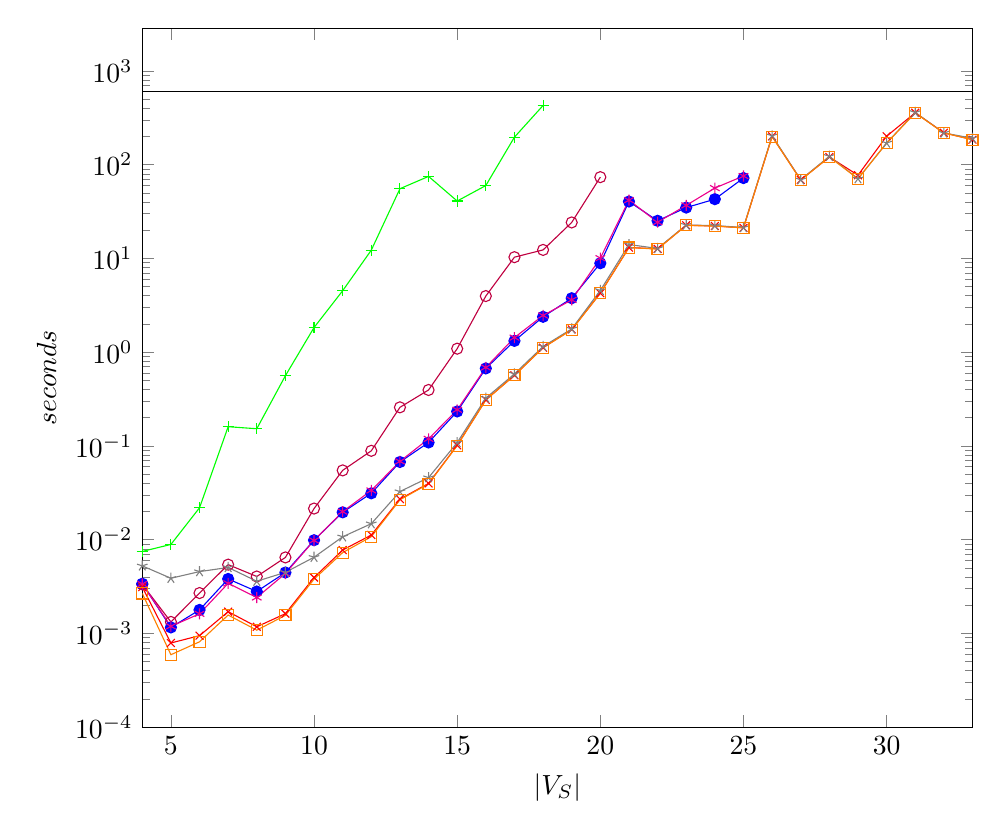
\begin{tikzpicture}
    \begin{axis}[
        xlabel=$|V_S|$,
        ylabel=$seconds$,
        ymin=0.0001,
        ymode=log,
        xmin=4,
        xmax=33,
        legend style={at={(0.9,0.1)},anchor=south east},
        width=\textwidth,
    ]
    
\addplot[
        mark=none,
        black,
    ] plot coordinates {
        (4,600)
        (33,600)
};
 %   \addlegendentry{Timeout 10m} 
    

    
   \addplot[
        mark=o,
        purple,
    ] plot coordinates {
        (4,0.0033354099999999996)
        (5,0.001327198)
        (6,0.0026972415)
        (7,0.005420836)
        (8,0.004050544)
        (9,0.006470579)
        (10,0.021485644)
        (11,0.0548721365)
        (12,0.0887547805)
        (13,0.258150266)
        (14,0.39556562399999995)
        (15,1.0907645185)
        (16,3.971699851282051)
        (17,10.321538780851064)
        (18,12.337433302040818)
        (19,24.217103684000005)
        (20,73.71199097)
};
%    \addlegendentry{GDFS O IP}
    
    
    
    \addplot[
        mark=+,
        green,
    ] plot coordinates {
        (4,0.0074964425000000005)
        (5,0.008899364)
        (6,0.021902257999999997)
        (7,0.160471234)
        (8,0.15263485899999998)
        (9,0.561916418)
        (10,1.833818564)
        (11,4.52718843880597)
        (12,12.26901466122449)
        (13,55.44448909999999)
        (14,75.0789921)
        (15,40.98504065555555)
        (16,59.94558265)
        (17,196.817508975)
        (18,428.4561328)
};
 %   \addlegendentry{CP}
    
    
    \addplot[
        mark=*,
        blue,
    ] plot coordinates {
        (4,0.0033891155)
        (5,0.0011595824999999999)
        (6,0.0017819205)
        (7,0.0038146409999999997)
        (8,0.0028014885)
        (9,0.004467115)
        (10,0.0098760425)
        (11,0.019585361000000003)
        (12,0.031251991)
        (13,0.067427614)
        (14,0.108922384)
        (15,0.233365984)
        (16,0.6713743385)
        (17,1.3210855519999998)
        (18,2.386009026)
        (19,3.765988756140351)
        (20,8.89447237352941)
        (21,40.502501818750005)
        (22,25.221025914285715)
        (23,34.883353815384616)
        (24,42.90160877142857)
        (25,72.07346983333335)
};
%    \addlegendentry{K-Path}
    
    \addplot[
        mark=asterisk,
        magenta,
    ] plot coordinates {
        (4,0.0033671915)
        (5,0.001190538)
        (6,0.0016191069999999998)
        (7,0.0034239325)
        (8,0.0024179585)
        (9,0.0043627885)
        (10,0.009817592)
        (11,0.019897870499999998)
        (12,0.0335268765)
        (13,0.068505526)
        (14,0.1189895675)
        (15,0.2430346145)
        (16,0.6879985279999999)
        (17,1.4320328555000001)
        (18,2.4644637565)
        (19,3.615006598192771)
        (20,10.072892529508197)
        (21,41.85573263125)
        (22,24.362516080952382)
        (23,36.84446636538462)
        (24,56.330943354545454)
        (25,75.77811247500001)
};
%    \addlegendentry{GDFS A IP}
    
    \addplot[
        mark=x,
        red,
    ] plot coordinates {
        (4,0.003124064)
        (5,7.913285000000001E-4)
        (6,9.468475E-4)
        (7,0.0017073364999999998)
        (8,0.0011771495)
        (9,0.0016255140000000002)
        (10,0.0039480825)
        (11,0.0077563585)
        (12,0.0112181135)
        (13,0.027106744)
        (14,0.039854954500000005)
        (15,0.1016730035)
        (16,0.3102863915)
        (17,0.567070922)
        (18,1.1181295875)
        (19,1.7503998269999999)
        (20,4.263310112765957)
        (21,13.087688980434784)
        (22,12.664759238095238)
        (23,22.604950978378376)
        (24,22.215862426666664)
        (25,21.221224975862068)
        (26,200.80231476666665)
        (27,69.01728853)
        (28,120.91195150000003)
        (29,77.2825083)
        (30,201.28251479999994)
        (31,358.3321691)
        (32,219.1503222)
        (33,184.9894481)
};
 %   \addlegendentry{DFS}
    
    \addplot[
        mark=star,
        gray,
    ] plot coordinates {
        (4,0.0052584419999999995)
        (5,0.0038800225)
        (6,0.0045671005)
        (7,0.005054851500000001)
        (8,0.0036043110000000002)
        (9,0.0044851380000000005)
        (10,0.006500158000000001)
        (11,0.010743765999999998)
        (12,0.014813136499999999)
        (13,0.032617665)
        (14,0.045932047000000004)
        (15,0.10862769200000001)
        (16,0.32415647649999996)
        (17,0.586893169)
        (18,1.1500186795)
        (19,1.772846179)
        (20,4.554298787121212)
        (21,14.077475467441861)
        (22,12.78838592857143)
        (23,22.725297256756754)
        (24,22.44824257)
        (25,21.37612426551724)
        (26,203.35969063333334)
        (27,69.08358688)
        (28,123.07605716000003)
        (29,70.88854776666666)
        (30,170.599628675)
        (31,361.26002704999996)
        (32,217.99103095)
        (33,191.6499955)
};
%    \addlegendentry{GDFS C}
    
    \addplot[
        mark=square,
        orange,
    ] plot coordinates {
        (4,0.0026720765000000004)
        (5,5.931255E-4)
        (6,8.145884999999999E-4)
        (7,0.0015716150000000002)
        (8,0.001083881)
        (9,0.0015602699999999999)
        (10,0.0037946819999999997)
        (11,0.0072780025)
        (12,0.010769405999999999)
        (13,0.026622686)
        (14,0.039441741499999995)
        (15,0.1005090725)
        (16,0.3088769205)
        (17,0.5658370635)
        (18,1.114951387)
        (19,1.7321635599999998)
        (20,4.2505378978723405)
        (21,13.068786297826087)
        (22,12.589129547619047)
        (23,22.530537545945947)
        (24,22.130406946666668)
        (25,21.19573636896552)
        (26,199.31648383333334)
        (27,68.44248519)
        (28,120.89257580000003)
        (29,70.80782896666666)
        (30,169.777134475)
        (31,356.8092052)
        (32,217.99103095)
        (33,184.9894481)
};
 %   \addlegendentry{portfolio}

    \end{axis}
    \end{tikzpicture}

\caption{$|V_T|=1\frac{1}{2}|V_S|$}
\end{subfigure}%
\begin{subfigure}{.5\linewidth}
\centering

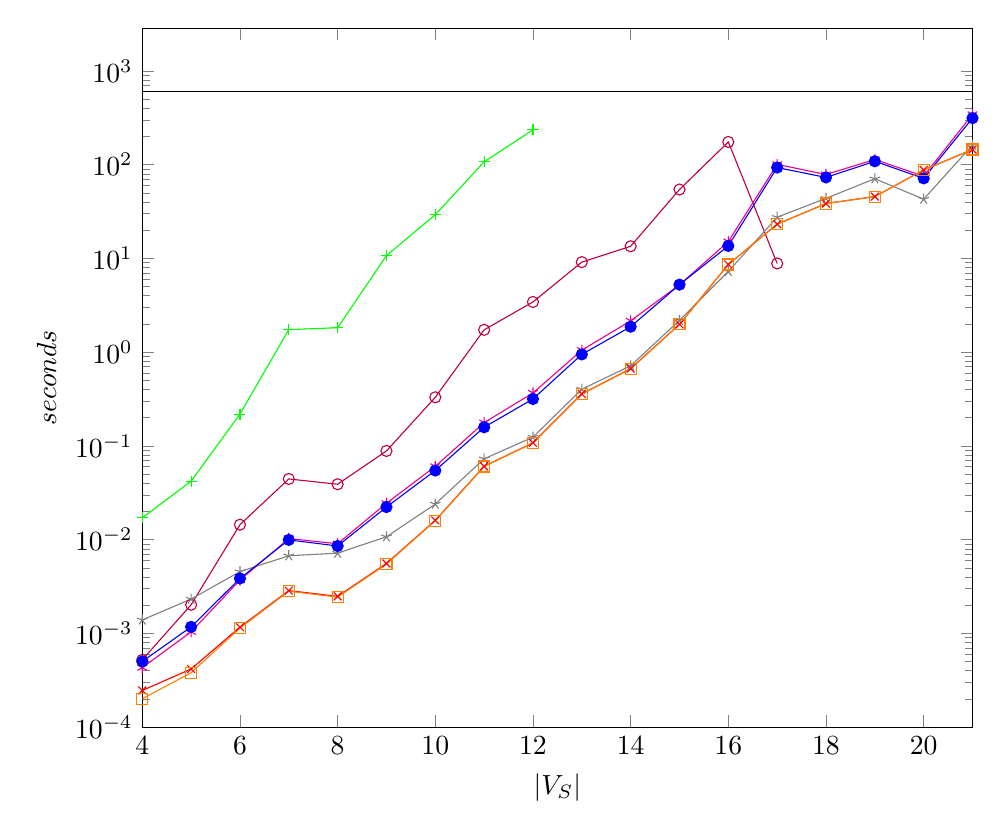
\begin{tikzpicture}
    \begin{axis}[
        xlabel=$|V_S|$,
        ylabel=$seconds$,
        ymin=0.0001,
        ymode=log,
        xmin=4,
        xmax=21,
        legend style={at={(0.9,0.1)},anchor=south east},
        width=\textwidth,
    ]
    
\addplot[
        mark=none,
        black,
    ] plot coordinates {
        (4,600)
        (21,600)
};
 %   \addlegendentry{Timeout 10m} 
    

\addplot[
        mark=+,
        green,
    ] plot coordinates {
        (4,0.017118874)
        (5,0.042044554000000005)
        (6,0.21861366149999997)
        (7,1.7413124975)
        (8,1.824231057)
        (9,10.718911422807018)
        (10,29.285856038095236)
        (11,107.36171433333334)
        (12,235.52224905)
};
%    \addlegendentry{CP}
    
    
    \addplot[
        mark=o,
        purple,
    ] plot coordinates {
        (4,5.229545E-4)
        (5,0.0020221634999999997)
        (6,0.014452913000000001)
        (7,0.044465508)
        (8,0.039038954)
        (9,0.088448429)
        (10,0.33017173499999997)
        (11,1.7330093685)
        (12,3.436815223163842)
        (13,9.139001624999999)
        (14,13.487728657446809)
        (15,54.37308013571429)
        (16,174.90209208000002)
        (17,8.8468752)
};
%    \addlegendentry{GDFS O IP}
    
    \addplot[
        mark=star,
        gray,
    ] plot coordinates {
        (4,0.00139258)
        (5,0.002327794)
        (6,0.004565538)
        (7,0.0067396635000000005)
        (8,0.0071890365)
        (9,0.010737805)
        (10,0.02400474)
        (11,0.07292148550000001)
        (12,0.12421214450000001)
        (13,0.403000701)
        (14,0.7163419985)
        (15,2.1890222930000003)
        (16,7.270705493975904)
        (17,27.538684308695654)
        (18,43.79655899583333)
        (19,70.8624523888889)
        (20,42.929491375)
        (21,161.7936666)
};
 %   \addlegendentry{GDFS C}
    
    \addplot[
        mark=x,
        red,
    ] plot coordinates {
        (4,2.463635E-4)
        (5,4.17268E-4)
        (6,0.001167168)
        (7,0.002865959)
        (8,0.0024855845)
        (9,0.0055816305)
        (10,0.016075872499999998)
        (11,0.060558201)
        (12,0.1081205275)
        (13,0.358527165)
        (14,0.6678748950000001)
        (15,1.9833789535)
        (16,8.623507047058824)
        (17,23.20956361923077)
        (18,38.53969741666666)
        (19,45.70503912307693)
        (20,88.00206148888888)
        (21,145.2799635)
};
%    \addlegendentry{DFS}
    
    
    \addplot[
        mark=asterisk,
        magenta,
    ] plot coordinates {
        (4,4.3166750000000006E-4)
        (5,0.0010404115)
        (6,0.003709151)
        (7,0.010290998499999999)
        (8,0.009050423)
        (9,0.0244776325)
        (10,0.060524060500000004)
        (11,0.177295532)
        (12,0.36728383800000003)
        (13,1.0505953314999998)
        (14,2.158745016)
        (15,5.232621873043478)
        (16,15.130776390697672)
        (17,100.89787280000002)
        (18,78.64249841111112)
        (19,113.64276582222222)
        (20,75.4335271625)
        (21,343.9340747)
};
%    \addlegendentry{GDFS A IP}
    
    \addplot[
        mark=*,
        blue,
    ] plot coordinates {
        (4,5.025650000000001E-4)
        (5,0.0011748805)
        (6,0.0038617564999999998)
        (7,0.009955469500000001)
        (8,0.008569285)
        (9,0.022299932)
        (10,0.054706759)
        (11,0.158324873)
        (12,0.317071005)
        (13,0.9476776635)
        (14,1.870529588)
        (15,5.256302935245901)
        (16,13.612862210869567)
        (17,93.2565386888889)
        (18,73.17322655555556)
        (19,108.78198909999999)
        (20,71.5219922)
        (21,314.1443365)
};
%    \addlegendentry{K-Path}
    
    \addplot[
        mark=square,
        orange,
    ] plot coordinates {
        (4,2.01024E-4)
        (5,3.8098600000000004E-4)
        (6,0.001139124)
        (7,0.0028233219999999996)
        (8,0.00244008)
        (9,0.0054960905)
        (10,0.015953537)
        (11,0.060388840000000006)
        (12,0.107574184)
        (13,0.358221664)
        (14,0.662612554)
        (15,1.9811704315)
        (16,8.621956076470587)
        (17,23.20956361923077)
        (18,38.53969741666666)
        (19,45.70503912307693)
        (20,88.00206148888888)
        (21,145.2799635)
};
 %   \addlegendentry{portfolio}
    

  
    \end{axis}
    \end{tikzpicture}

\caption{$|V_T|=3|V_S|$}
\end{subfigure}\\[1ex]
\begin{subfigure}{0.5\linewidth}
\centering

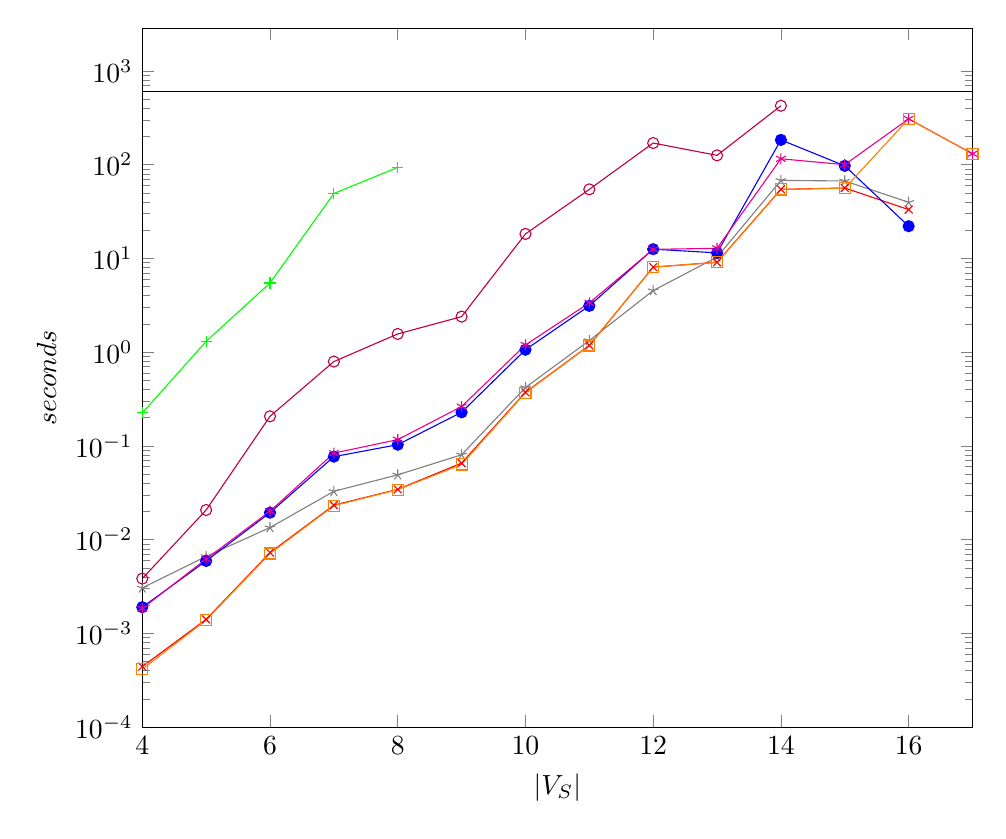
\begin{tikzpicture}
    \begin{axis}[
        xlabel=$|V_S|$,
        ylabel=$seconds$,
        ymin=0.0001,
        ymode=log,
        xmin=4,
        xmax=17,
        legend style={at={(0.9,0.1)},anchor=south east},
        width=\textwidth,
    ]
    
\addplot[
        mark=none,
        black,
    ] plot coordinates {
        (4,600)
        (17,600)
};
 %   \addlegendentry{Timeout 10m} 
    


\addplot[
        mark=+,
        green,
    ] plot coordinates {
        (4,0.22498123849999999)
        (5,1.305544137)
        (6,5.477192146428571)
        (7,49.320910733333335)
        (8,93.62391244)
};
%    \addlegendentry{CP}
    
    
    \addplot[
        mark=star,
        gray,
    ] plot coordinates {
        (4,0.003058187)
        (5,0.0066316019999999995)
        (6,0.013466777000000001)
        (7,0.032822169)
        (8,0.049183345)
        (9,0.080513419)
        (10,0.4200455685)
        (11,1.3332708905000001)
        (12,4.545143440151515)
        (13,10.333796216470589)
        (14,68.03150406)
        (15,67.08428195454545)
        (16,39.747431)
};
%    \addlegendentry{GDFS C}
    
    \addplot[
        mark=x,
        red,
    ] plot coordinates {
        (4,4.4261750000000003E-4)
        (5,0.0014131274999999999)
        (6,0.0072753685000000005)
        (7,0.023372011)
        (8,0.0344219615)
        (9,0.0656533275)
        (10,0.3738274895)
        (11,1.183567724)
        (12,8.084725380597014)
        (13,9.105788104705884)
        (14,54.59190611666667)
        (15,56.45855956363636)
        (16,33.2144619)
};
%    \addlegendentry{DFS}
    
    \addplot[
        mark=*,
        blue,
    ] plot coordinates {
        (4,0.001906137)
        (5,0.005935332)
        (6,0.0194225855)
        (7,0.0768926385)
        (8,0.103136142)
        (9,0.228699563)
        (10,1.062870499)
        (11,3.1228105518134712)
        (12,12.555450586)
        (13,11.474581472222223)
        (14,183.9983442333333)
        (15,97.27099918571427)
        (16,22.0919737)
};
%    \addlegendentry{K-Path}
    
    
    \addplot[
        mark=o,
        purple,
    ] plot coordinates {
        (4,0.0038459365)
        (5,0.020740273)
        (6,0.20711417999999998)
        (7,0.7947821999999999)
        (8,1.565915889)
        (9,2.396293172)
        (10,18.270429463636365)
        (11,54.59309324615385)
        (12,170.3045068)
        (13,125.79853659999999)
        (14,425.516946)
};
%    \addlegendentry{GDFS O IP}
    
    
    \addplot[
        mark=asterisk,
        magenta,
    ] plot coordinates {
        (4,0.0018444635000000001)
        (5,0.006224887500000001)
        (6,0.0201156265)
        (7,0.0838507)
        (8,0.11677660100000001)
        (9,0.2631939955)
        (10,1.195823311)
        (11,3.358671161111111)
        (12,12.508858883333334)
        (13,12.832528379245282)
        (14,115.64856344)
        (15,100.09827916666666)
        (16,308.21460745)
        (17,130.7677965)
};
%    \addlegendentry{GDFS A IP}
    
    
    \addplot[
        mark=square,
        orange,
    ] plot coordinates {
        (4,4.152115E-4)
        (5,0.001389112)
        (6,0.0071271165)
        (7,0.023055476000000002)
        (8,0.034188356)
        (9,0.0634472525)
        (10,0.370240898)
        (11,1.1794381704999999)
        (12,8.077388874626866)
        (13,9.088254795294118)
        (14,54.45241678333334)
        (15,56.29606548181818)
        (16,308.21460745)
        (17,130.7677965)
};
%    \addlegendentry{portfolio}
    
  
    \end{axis}
    \end{tikzpicture}

\caption{$|V_T|=5|V_S|$}
\end{subfigure}
\begin{subfigure} {0.5\linewidth}
\centering

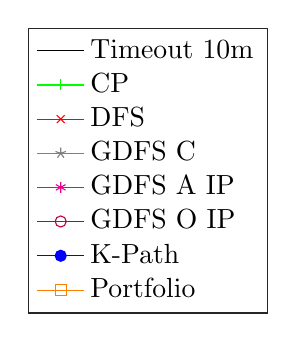
\begin{tikzpicture} 
    \begin{axis}[%
    hide axis,
    xmin=10,
    xmax=50,
    ymin=0,
    ymax=0.4,
    legend style={draw=white!15!black,legend cell align=left}
    ]
	\addlegendimage{black}
    \addlegendentry{Timeout 10m}; 
     
    \addlegendimage{green, mark=+}
    \addlegendentry{CP};
    
    \addlegendimage{red, mark=x}
    \addlegendentry{DFS};
    
    \addlegendimage{gray, mark=star}
    \addlegendentry{GDFS C};
    
    \addlegendimage{magenta, mark=asterisk}
    \addlegendentry{GDFS A IP};
    
    \addlegendimage{purple, mark=o}
    \addlegendentry{GDFS O IP};
    
    \addlegendimage{blue, mark=*}
    \addlegendentry{K-Path};
    
    \addlegendimage{orange, mark=square}
    \addlegendentry{Portfolio};
    \end{axis}
\end{tikzpicture}

\end{subfigure}
\caption{Performance of using different path iterators in test cases with present subgraph homeomorphisms. We avoid unnecessarily long paths, and use no pruning or contraction. We include a portfolio method that takes the best performance rating for each individual test case.}	
\label{fig:pathiterator-performance}
\end{figure}


\begin{figure}
\centering
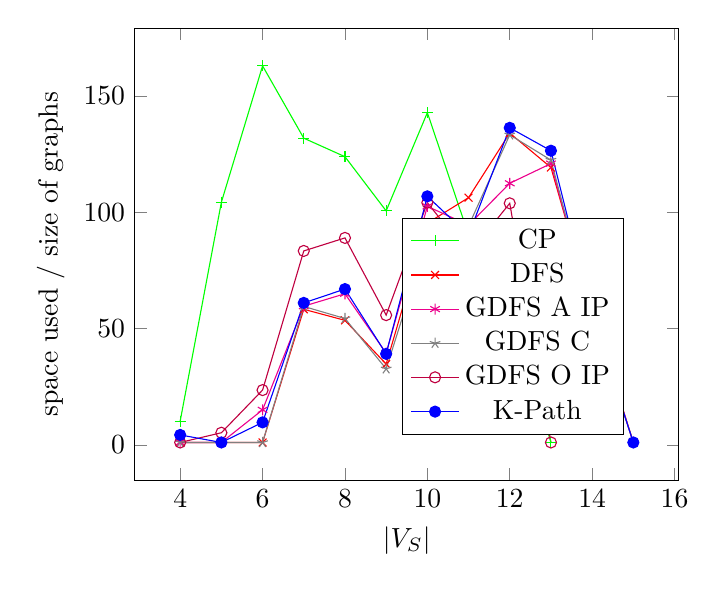
\begin{tikzpicture}
    \begin{axis}[
        xlabel=$|V_S|$,
        ylabel=space used $/$ size of graphs,
        legend style={at={(0.9,0.1)},anchor=south east},
        width=0.7\textwidth,
		%y tick label style={/pgf/number format/sci},
    ]

%    \node[] at (axis cs: 9,1.1) {Awaiting test results (CAES server)};

\addplot[
        mark=+,
        green,
    ] plot coordinates {
        (4,10.174505370550349224253838)
        (5,104.28268407548150313423625)
        (6,162.90001905722773387141976)
        (7,131.82092679714642689897069)
        (8,123.86131153662219616440982)
        (9,100.54876902079979411614113)
        (10,142.8055123071906161809092)
        (11,90.23704183358028315864566)
        (12,60.13828770787494509749228)
        (13,1)
};
    \addlegendentry{CP}
    
    \addplot[
        mark=x,
        red,
    ] plot coordinates {
        (4,1)
        (5,1)
        (6,1)
        (7,58.25769782075416109734502296)
        (8,53.49977853854609387401796491)
        (9,34.69315781105574763597362315)
        (10,95.2821470489074655940527300)
        (11,106.247669775327306151566700)
        (12,134.009989654390014925155652)
        (13,119.208253326512152230628507)
        (14,57.5163619146955535818220329)
        (15,1)
};
    \addlegendentry{DFS}

    \addplot[
        mark=asterisk,
        magenta,
    ] plot coordinates {
        (4,1)
        (5,1)
        (6,15.02985034471161930)
        (7,59.59097376035428638)
        (8,64.93368304714666954)
        (9,39.37678578646825642)
        (10,102.493087611314720)
        (11,94.4701670636009438)
        (12,112.425234638110666)
        (13,120.892092891415954)
        (14,56.0582514421801884)
        (15,1)
};
    \addlegendentry{GDFS A IP}
    
    \addplot[
        mark=star,
        gray,
    ] plot coordinates {
        (4,1)
        (5,1)
        (6,1)
        (7,59.479189954442690)
        (8,54.294753873478837)
        (9,32.656874607567579)
        (10,88.62263521222060)
        (11,94.07313175657136)
        (12,133.2439360650590)
        (13,122.4129802403613)
        (14,55.53333167207465)
        (15,1)
};
    \addlegendentry{GDFS C}
    
    \addplot[
        mark=o,
        purple,
    ] plot coordinates {
        (4,1)
        (5,5.1826054759816817)
        (6,23.512962277899220)
        (7,83.341983867316274)
        (8,88.941938162115534)
        (9,55.750056887542679)
        (10,104.1015790897492)
        (11,81.84559512703726)
        (12,103.8155851653250)
        (13,1)
};
    \addlegendentry{GDFS O IP}
    
    \addplot[
        mark=*,
        blue,
    ] plot coordinates {
        (4,4.240778515784331992)
        (5,1)
        (6,9.641524578218709713)
        (7,61.00961187901417579)
        (8,66.94762056230962072)
        (9,39.09244788901674288)
        (10,106.812982924035309)
        (11,90.1677790988596005)
        (12,136.268506857638343)
        (13,126.432468234002608)
        (14,55.5333316720746569)
        (15,1)
};
    \addlegendentry{K-Path}
	
    \end{axis}
    \end{tikzpicture}
    \caption{Space usage of the algorithm with each path iterator relative to the space usage of the input graphs. Unnecessarily long paths are avoided, target vertices are ordered by degree and contraction is disabled.}
    \label{fig:spaceusage-pathiterators}

\end{figure}



\begin{figure}
\begin{subfigure}{.5\linewidth}
\centering

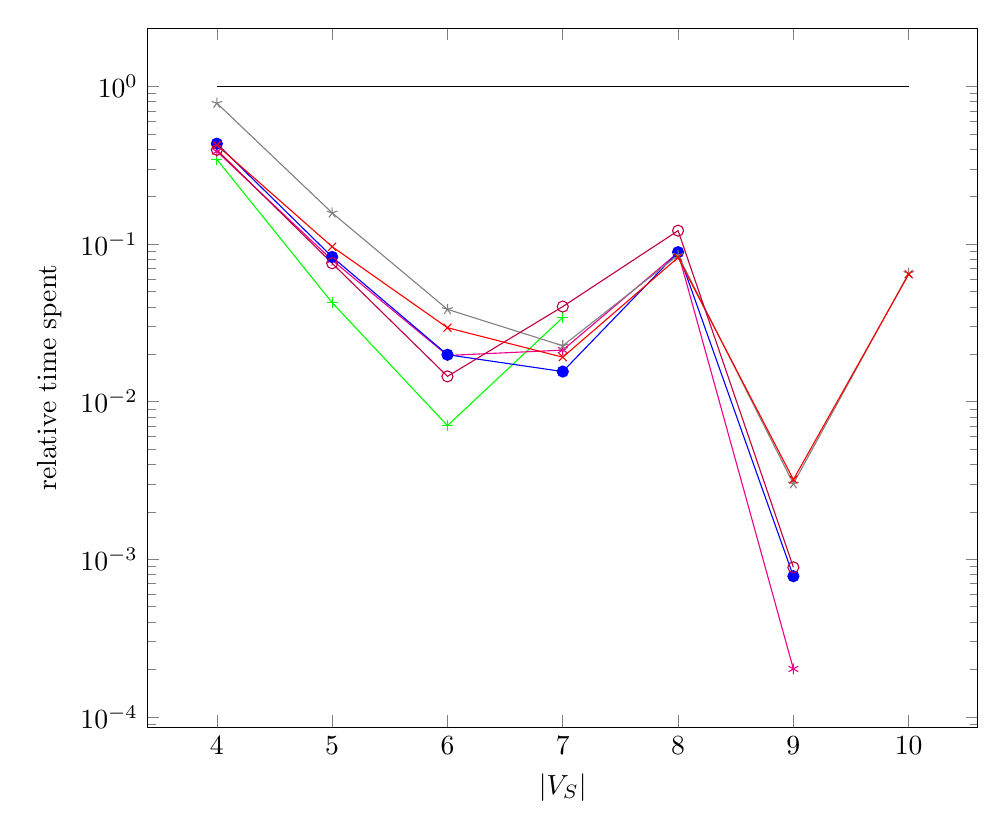
\begin{tikzpicture}
    \begin{axis}[
        xlabel=$|V_S|$,
        ylabel=relative time spent,
        ymode=log,
        legend style={at={(0.9,0.1)},anchor=south east},
        width=\textwidth,
		y tick label style={/pgf/number format/sci},
    ]


\addplot [mark=none, black] plot coordinates {
        (4,1) (10, 1)};
%\addlegendentry{No contraction}
   \addplot[
        mark=+,
        green,
    ] plot coordinates {
        (4,0.34449583915246557)
        (5,0.04250500407360703)
        (6,0.007052140364736389)
        (7,0.034219490143735744)
};
%    \addlegendentry{CP}

\addplot[
        mark=asterisk,
        magenta,
    ] plot coordinates {
        (4,0.38742564587487976)
        (5,0.07909766239343824)
        (6,0.019655091474591525)
        (7,0.021251734957033044)
        (8,0.08842360246711035)
        (9,2.0164236395563237E-4)
};
%    \addlegendentry{GDFS A IP}

\addplot[
        mark=*,
        blue,
    ] plot coordinates {
        (4,0.43377165034858706)
        (5,0.08291766655357158)
        (6,0.019867063872060407)
        (7,0.01553750194233227)
        (8,0.08890227690765527)
        (9,7.816551173891351E-4)
};
%    \addlegendentry{K-Path}

\addplot[
        mark=star,
        gray,
    ] plot coordinates {
        (4,0.7838841422440458)
        (5,0.15772533322419885)
        (6,0.03853822820095056)
        (7,0.02265222193749682)
        (8,0.08504004296545455)
        (9,0.0030177729737449885)
        (10,0.0652985451968477)
};
%    \addlegendentry{GDFS C}

\addplot[
        mark=x,
        red,
    ] plot coordinates {
        (4,0.42425950110101485)
        (5,0.09626130731943527)
        (6,0.029475512058189532)
        (7,0.019168059826692858)
        (8,0.08213870898979722)
        (9,0.00320538172801908)
        (10,0.06429911639723773)
};
%    \addlegendentry{DFS}

\addplot[
        mark=o,
        purple,
    ] plot coordinates {
        (4,0.3963989888723202)
        (5,0.07559274867485685)
        (6,0.014479163749969607)
        (7,0.04015195913379275)
        (8,0.12166475428162647)
        (9,8.901952837352006E-4)
};
%    \addlegendentry{GDFS O IP}


    \end{axis}
    \end{tikzpicture}


\caption{$|V_T|=1\frac{1}{2}|V_S|$}
\end{subfigure}%
\begin{subfigure}{.5\linewidth}
\centering

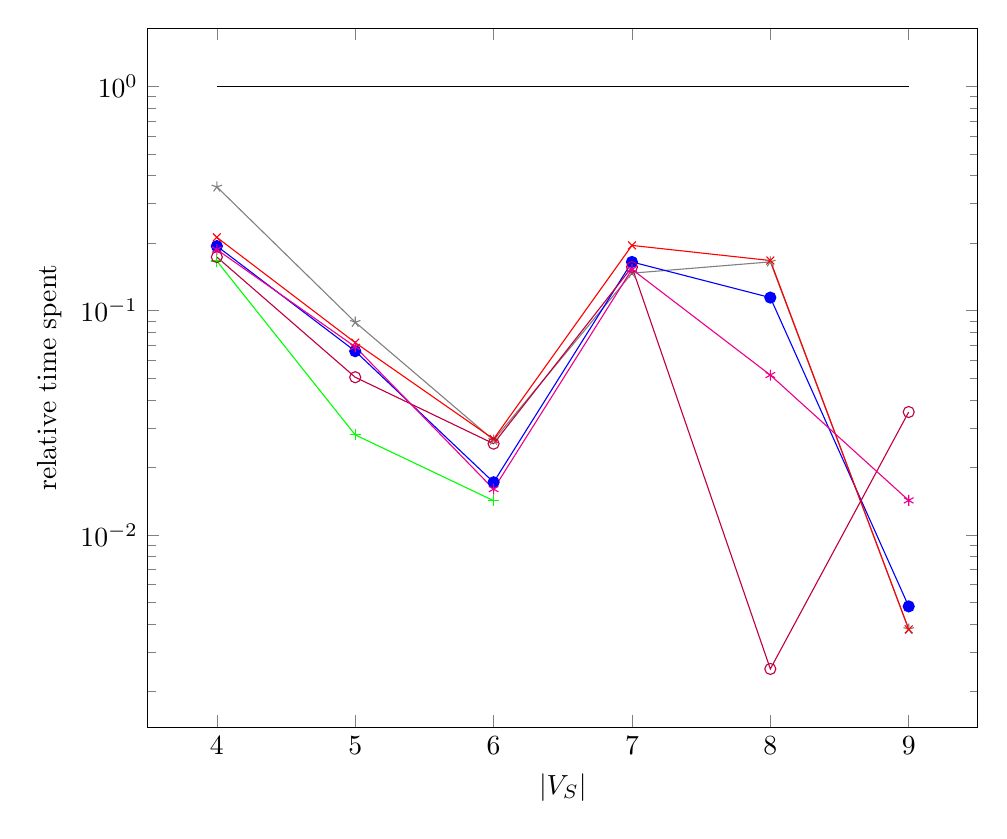
\begin{tikzpicture}
    \begin{axis}[
        xlabel=$|V_S|$,
        ylabel=relative time spent,
        ymode=log,
        legend style={at={(0.9,0.1)},anchor=south east},
        width=\textwidth,
		y tick label style={/pgf/number format/sci},
    ]


\addplot [mark=none, black] plot coordinates {
        (4,1) (9, 1)};
%\addlegendentry{No contraction}

\addplot[
        mark=+,
        green,
    ] plot coordinates {
        (4,0.16656533269519228)
        (5,0.02792481959372131)
        (6,0.014208494420317713)
};
%    \addlegendentry{CP}

\addplot[
        mark=star,
        gray,
    ] plot coordinates {
        (4,0.35670503391181074)
        (5,0.08885285052563148)
        (6,0.02644959281461509)
        (7,0.1469727809071855)
        (8,0.1650715123096471)
        (9,0.003794253797042311)
};
%    \addlegendentry{GDFS C}

\addplot[
        mark=*,
        blue,
    ] plot coordinates {
        (4,0.194158851426724)
        (5,0.06596676865264874)
        (6,0.017166588789163415)
        (7,0.16493104718190343)
        (8,0.11438599305894)
        (9,0.0047972337258095485)
};
%    \addlegendentry{K-Path}

\addplot[
        mark=x,
        red,
    ] plot coordinates {
        (4,0.21233351678836204)
        (5,0.07202295158409817)
        (6,0.026758726043938773)
        (7,0.19551506606564623)
        (8,0.16739005564904727)
        (9,0.003790913734381372)
};
%    \addlegendentry{DFS}

\addplot[
        mark=o,
        purple,
    ] plot coordinates {
        (4,0.17347891126074652)
        (5,0.0504791507537965)
        (6,0.02551664872425517)
        (7,0.15650709939163068)
        (8,0.0025235131787816165)
        (9,0.03532832186507143)
};
%    \addlegendentry{GDFS O IP}

\addplot[
        mark=asterisk,
        magenta,
    ] plot coordinates {
        (4,0.1873514680576187)
        (5,0.06902784077974626)
        (6,0.0160036619729299)
        (7,0.15291763768405797)
        (8,0.0516269965234984)
        (9,0.014247055717867137)
};
%    \addlegendentry{GDFS A IP}
	
	
    \end{axis}
    \end{tikzpicture}

\caption{$|V_T|=3|V_S|$}
\end{subfigure}\\[1ex]
\begin{subfigure}{0.5\linewidth}
\centering

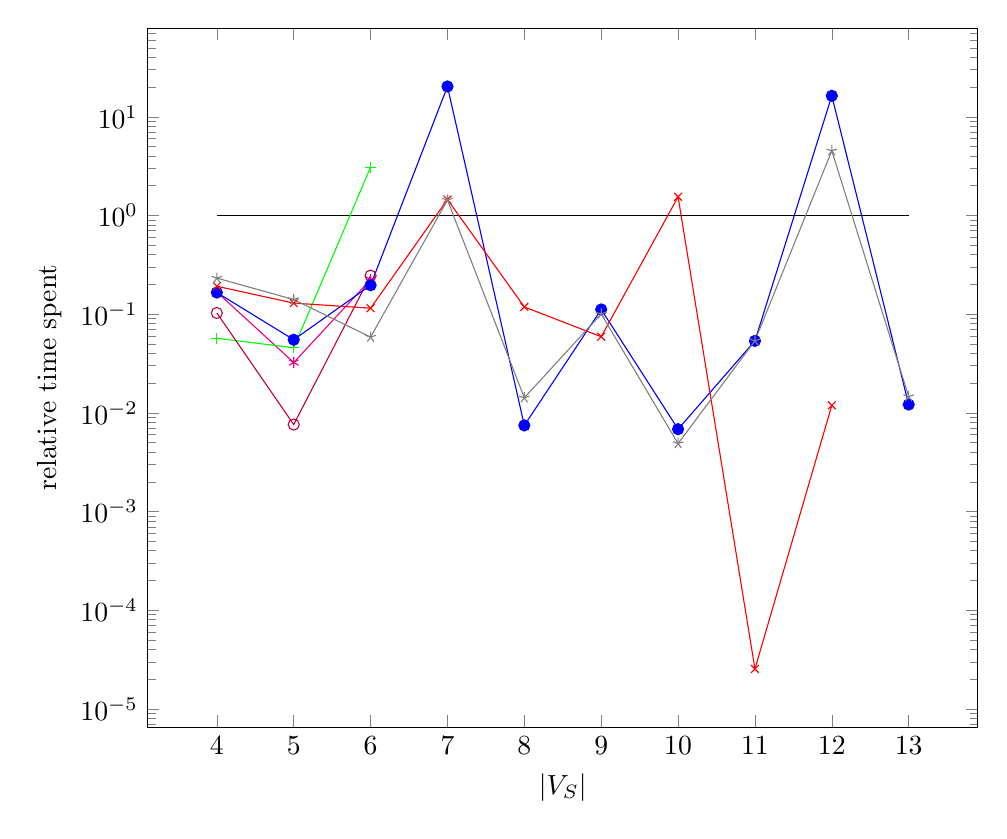
\begin{tikzpicture}
    \begin{axis}[
        xlabel=$|V_S|$,
        ylabel=relative time spent,
        ymode=log,
        legend style={at={(0.9,0.1)},anchor=south east},
        width=\textwidth,
		y tick label style={/pgf/number format/sci},
    ]


\addplot [mark=none, black] plot coordinates {
        (4,1) (13, 1)};
%\addlegendentry{No contraction}

	
\addplot[
        mark=asterisk,
        magenta,
    ] plot coordinates {
        (4,0.1674566113900499)
        (5,0.032349725367020715)
        (6,0.2237865876374895)
};
 %   \addlegendentry{GDFS A IP}
    
    
    \addplot[
        mark=+,
        green,
    ] plot coordinates {
        (4,0.056873208163624955)
        (5,0.04563421043002553)
        (6,3.0895140030860113)
};
 %   \addlegendentry{CP}
    
    \addplot[
        mark=o,
        purple,
    ] plot coordinates {
        (4,0.10276640004366641)
        (5,0.007609829164036706)
        (6,0.24568669245593505)
};
 %   \addlegendentry{GDFS O IP}
    
    \addplot[
        mark=*,
        blue,
    ] plot coordinates {
        (4,0.1655772370426709)
        (5,0.055053818828159615)
        (6,0.19634060714182988)
        (7,20.289869886299307)
        (8,0.007455438509609334)
        (9,0.11168570137538518)
        (10,0.006832180347245251)
        (11,0.053585054708433756)
        (12,16.326793831579934)
        (13,0.01212843469374362)
};
 %   \addlegendentry{K-Path}


\addplot[
        mark=x,
        red,
    ] plot coordinates {
        (4,0.19178983176776473)
        (5,0.1293662743185925)
        (6,0.11496995869605499)
        (7,1.450331503028158)
        (8,0.11835078397595038)
        (9,0.05907513412579321)
        (10,1.545090436667155)
        (11,2.5391954884407796E-5)
        (12,0.011908323973143663)
};
 %   \addlegendentry{DFS}
    
    \addplot[
        mark=star,
        gray,
    ] plot coordinates {
        (4,0.23202692835799185)
        (5,0.14055133962348276)
        (6,0.05857415542176621)
        (7,1.4332274024971468)
        (8,0.014217322662230782)
        (9,0.10041348158626583)
        (10,0.004884744036490124)
        (11,0.053666528274866135)
        (12,4.5260118047084195)
        (13,0.01461043009387195)
};
%    \addlegendentry{GDFS C}
	
	
    \end{axis}
    \end{tikzpicture}

\caption{$|V_T|=5|V_S|$}
\end{subfigure}
\begin{subfigure} {0.5\linewidth}
\centering

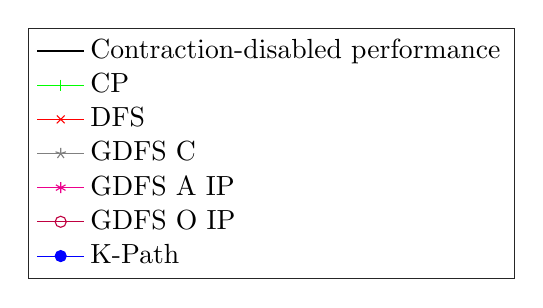
\begin{tikzpicture} 
    \begin{axis}[%
    hide axis,
    xmin=10,
    xmax=50,
    ymin=0,
    ymax=0.4,
    legend style={draw=white!15!black,legend cell align=left}
    ]
	\addlegendimage{black}
    \addlegendentry{Contraction-disabled performance}; 
     
    \addlegendimage{green, mark=+}
    \addlegendentry{CP};
    
    \addlegendimage{red, mark=x}
    \addlegendentry{DFS};
    
    \addlegendimage{gray, mark=star}
    \addlegendentry{GDFS C};
    
    \addlegendimage{magenta, mark=asterisk}
    \addlegendentry{GDFS A IP};
    
    \addlegendimage{purple, mark=o}
    \addlegendentry{GDFS O IP};
    
    \addlegendimage{blue, mark=*}
    \addlegendentry{K-Path};
    
    \end{axis}
\end{tikzpicture}

\end{subfigure}

\caption{Performance of our algorithm with the GreatestConstrainedFirst source graph vertex order relative to the performance of the algorithm with a random source graph vertex order. We avoid unnecessarily long paths, do not perform contraction and use no pruning. Data points above the black reference line denote the GreatestConstrainedFirst ordering introduces more delay, and data points below the reference line denote that it saves time. Note the logarithmic y-axis.}	
\label{fig:greatestConstrainedfirstVersusRandom}
\end{figure}




\begin{figure}
\resizebox{0.28\textheight}{!}{
\begin{subfigure}{.5\linewidth}
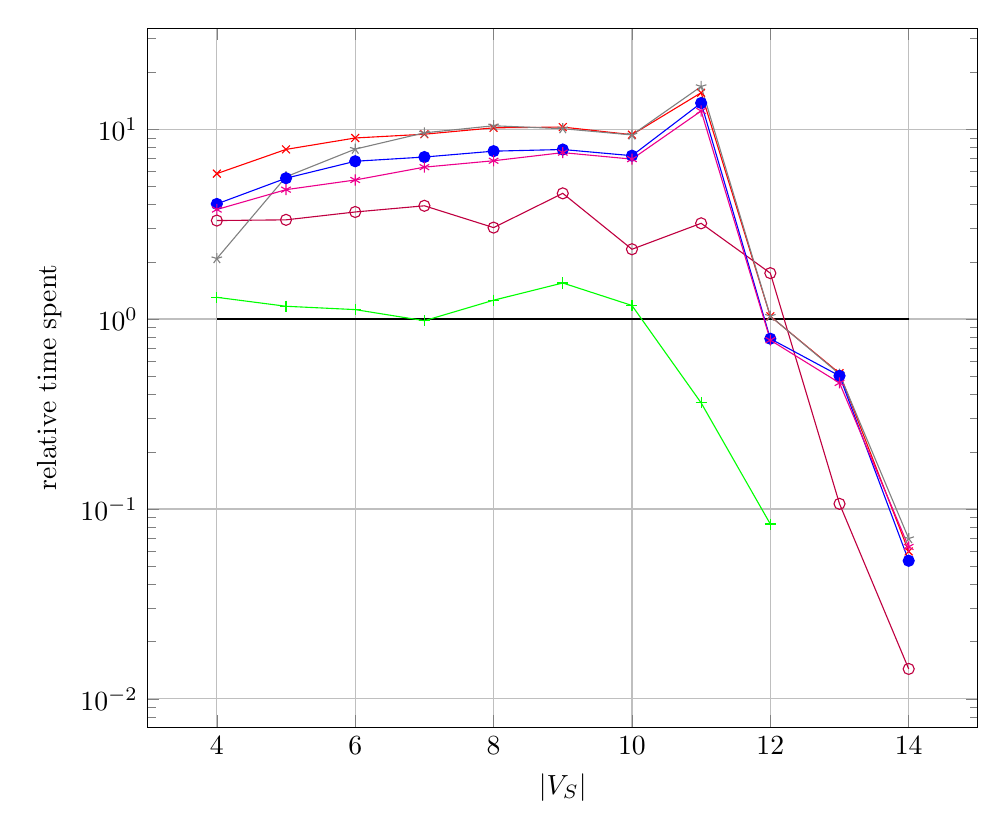
\begin{tikzpicture}
    \begin{axis}[
        xlabel=$|V_S|$,
        ylabel=relative time spent,
        ymode=log,
        legend style={at={(0.9,0.1)},anchor=south east},
        width=\textwidth,
		y tick label style={/pgf/number format/sci},
        ymajorgrids,
        xmajorgrids,		
    ]
\addplot [mark=none, black] plot coordinates {
        (4,1) (14,1)};




\addplot[
        mark=x,
        red,
    ] plot coordinates {
        (4,5.829952304363644)
        (5,7.821514135009583)
        (6,8.982363969917358)
        (7,9.401332680691212)
        (8,10.158832279951605)
        (9,10.252325251025706)
        (10,9.34581888789391)
        (11,15.546748123060839)
        (12,1.0341526662898237)
        (13,0.5183898969146863)
        (14,0.05971709064829511)
};
%    \addlegendentry{DFS}


\addplot[
        mark=o,
        purple,
    ] plot coordinates {
        (4,3.3007473913750918)
        (5,3.3292641262270837)
        (6,3.6622616535723047)
        (7,3.9481137630108396)
        (8,3.030286162147374)
        (9,4.590014716545663)
        (10,2.330905974473567)
        (11,3.192281658331693)
        (12,1.744595348175264)
        (13,0.10640200382876541)
        (14,0.014374937918376296)
};
%    \addlegendentry{GDFS O IP}


\addplot[
        mark=star,
        gray,
    ] plot coordinates {
        (4,2.081240181067252)
        (5,5.613910854682754)
        (6,7.849457219522296)
        (7,9.56049923079753)
        (8,10.416398040783026)
        (9,10.0534722450281)
        (10,9.318833737054117)
        (11,16.77294360448037)
        (12,1.036148432755423)
        (13,0.5131767288245823)
        (14,0.06986347139547233)
};
%    \addlegendentry{GDFS C}


\addplot[
        mark=*,
        blue,
    ] plot coordinates {
        (4,4.036935610516745)
        (5,5.515429351367027)
        (6,6.774063252800069)
        (7,7.129623094348765)
        (8,7.656237850184846)
        (9,7.811733342175969)
        (10,7.246802908944303)
        (11,13.722983859104243)
        (12,0.7878416162899551)
        (13,0.502222694200184)
        (14,0.053345329755408066)
};
%    \addlegendentry{K-Path}
\addplot[
        mark=+,
        green,
    ] plot coordinates {
        (4,1.3011349314115381)
        (5,1.1674190431355977)
        (6,1.1211917642297184)
        (7,0.9799097022873059)
        (8,1.2563225326740295)
        (9,1.5481480597546917)
        (10,1.17848246411115)
        (11,0.3618711611946529)
        (12,0.08327602042560134)
};
%    \addlegendentry{CP}


\addplot[
        mark=asterisk,
        magenta,
    ] plot coordinates {
        (4,3.7736038154304787)
        (5,4.800389319350771)
        (6,5.397341566198895)
        (7,6.306734163350917)
        (8,6.815885755656629)
        (9,7.520888523608972)
        (10,6.951520443072349)
        (11,12.458753170545519)
        (12,0.7742934930427632)
        (13,0.46088425014379175)
        (14,0.06313695543283937)
};
%    \addlegendentry{GDFS A IP}





    \end{axis}
    \end{tikzpicture}
\caption{$|V_T|=1\frac{1}{2}*|V_S|$ (no caching)}
\end{subfigure}%
}
\resizebox{0.28\textheight}{!}{
\begin{subfigure}{.5\linewidth}
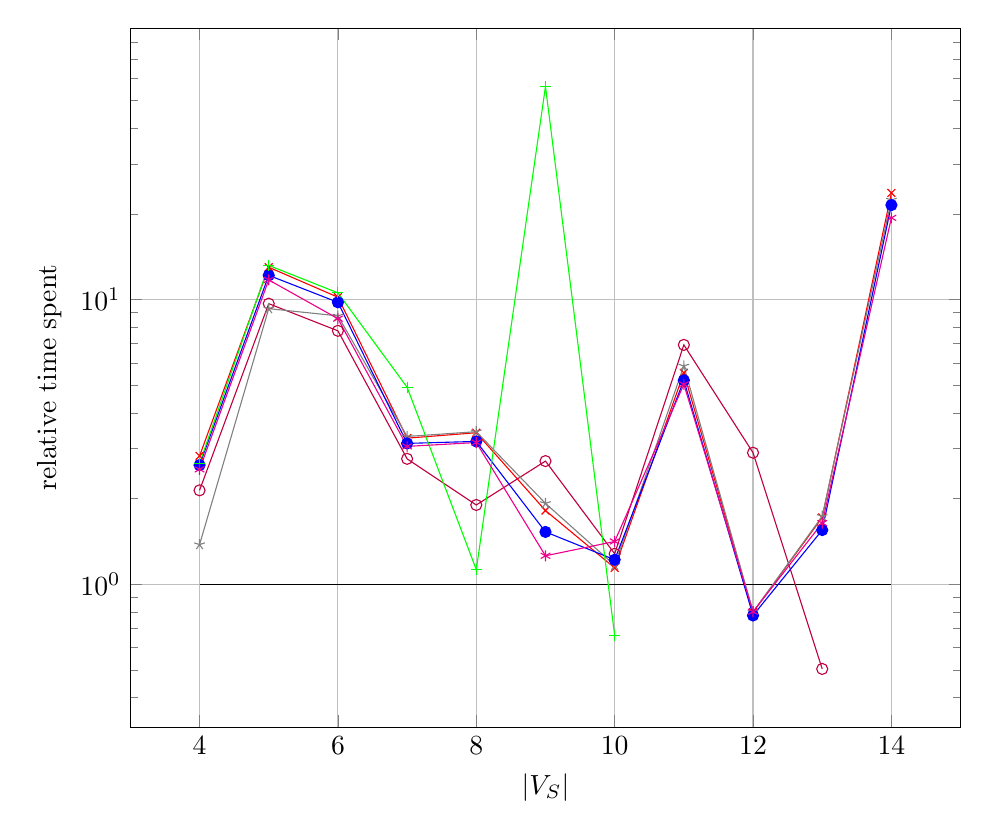
\begin{tikzpicture}
    \begin{axis}[
        xlabel=$|V_S|$,
        ylabel=relative time spent,
        ymode=log,
        legend style={at={(0.9,0.1)},anchor=south east},
        width=\textwidth,
		y tick label style={/pgf/number format/sci},
        ymajorgrids,
        xmajorgrids,		
    ]
\addplot [mark=none, black] plot coordinates {
        (4,1) (14, 1)};





\addplot[
        mark=x,
        red,
    ] plot coordinates {
        (4,2.8251795368790886)
        (5,12.999580346656751)
        (6,10.202174684933484)
        (7,3.262604211259584)
        (8,3.408918438863976)
        (9,1.8166545299203807)
        (10,1.1422160886456934)
        (11,5.530516473257274)
        (12,0.7986133987525276)
        (13,1.7180491450318693)
        (14,23.721522460227753)
};
%    \addlegendentry{DFS}
\addplot[
        mark=o,
        purple,
    ] plot coordinates {
        (4,2.1391785196119923)
        (5,9.683057001857964)
        (6,7.773825041515071)
        (7,2.7604466990768595)
        (8,1.9008757163878494)
        (9,2.7101513865191915)
        (10,1.2805148059566114)
        (11,6.937603075441524)
        (12,2.9004853202789205)
        (13,0.5045390730335063)
};
%    \addlegendentry{GDFS O IP}


\addplot[
        mark=star,
        gray,
    ] plot coordinates {
        (4,1.3794140730076914)
        (5,9.299733094390856)
        (6,8.772951593738188)
        (7,3.307376496667975)
        (8,3.4383266889141892)
        (9,1.9254251970590692)
        (10,1.1671557982423402)
        (11,5.851599859841392)
        (12,0.7997588706522294)
        (13,1.7348281924961175)
        (14,22.40100510075956)
};
%    \addlegendentry{GDFS C}


\addplot[
        mark=*,
        blue,
    ] plot coordinates {
        (4,2.6239880026319113)
        (5,12.176055240511092)
        (6,9.786244499035096)
        (7,3.127359936505137)
        (8,3.1774880567968005)
        (9,1.528458868204552)
        (10,1.2199898778953424)
        (11,5.209122239775357)
        (12,0.7776618244283469)
        (13,1.5513809856510496)
        (14,21.49466036911607)
};
%    \addlegendentry{K-Path}


\addplot[
        mark=+,
        green,
    ] plot coordinates {
        (4,2.6615145962479296)
        (5,13.192185281822104)
        (6,10.56726292801845)
        (7,4.92388122723026)
        (8,1.126596319598566)
        (9,56.0969304160683)
        (10,0.6621016861467689)
};
%    \addlegendentry{CP}


\addplot[
        mark=asterisk,
        magenta,
    ] plot coordinates {
        (4,2.5345706323293955)
        (5,11.732948804586153)
        (6,8.577253069471816)
        (7,3.052311500224188)
        (8,3.1492268511393373)
        (9,1.2598729843415928)
        (10,1.414481795839197)
        (11,5.042048634623404)
        (12,0.8013450614402682)
        (13,1.642270880020916)
        (14,19.386486921496203)
};
%    \addlegendentry{GDFS A IP}



	
    \end{axis}
    \end{tikzpicture}

\caption{$|V_T|=1\frac{1}{2}*|V_S|$ (cached)}
\end{subfigure}
}
\newline
\resizebox{0.28\textheight}{!}{
\begin{subfigure}{0.5\linewidth}

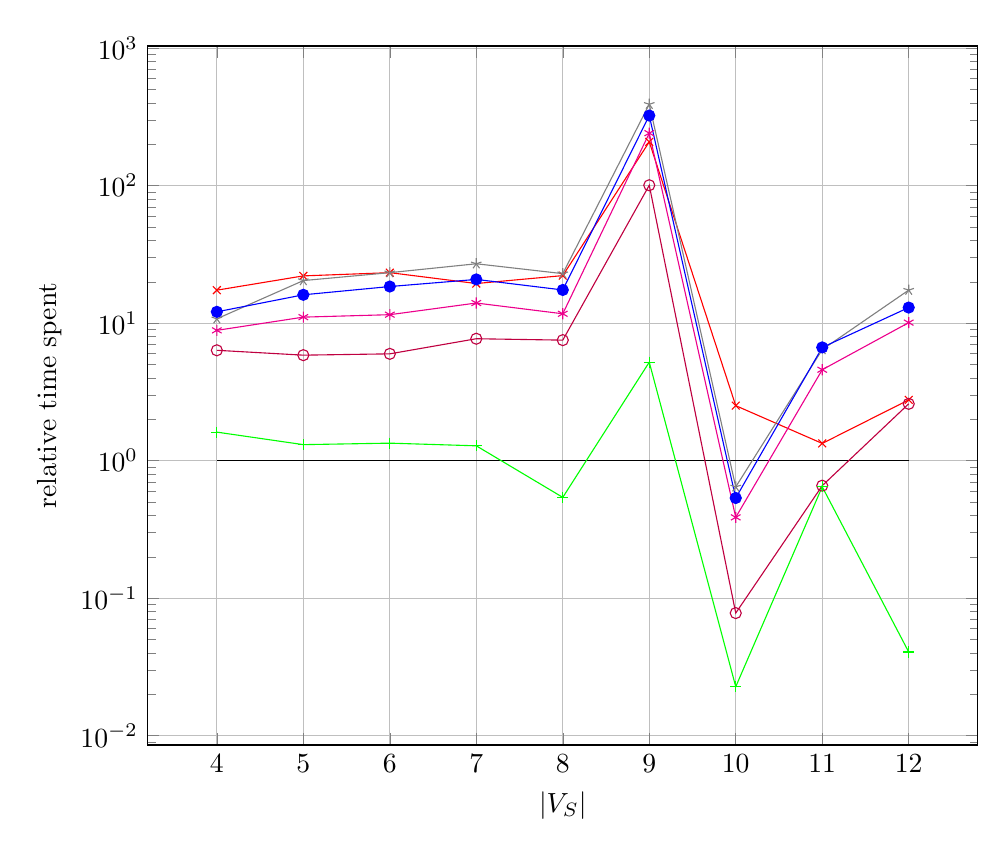
\begin{tikzpicture}
    \begin{axis}[
        xlabel=$|V_S|$,
        ylabel=relative time spent,
        ymode=log,
        legend style={at={(0.9,0.1)},anchor=south east},
        width=\textwidth,
		y tick label style={/pgf/number format/sci},
        ymajorgrids,
        xmajorgrids,		
    ]
\addplot [mark=none, black] plot coordinates {
        (4,1) (12, 1)};
        
%    \node[] at (axis cs: 9,1.1) {Awaiting test results (CAES server)};


\addplot[
        mark=x,
        red,
    ] plot coordinates {
        (4,17.386687830540524)
        (5,22.079291788970327)
        (6,23.306743149976228)
        (7,19.430501058064742)
        (8,22.18188165942091)
        (9,208.2138028355397)
        (10,2.513700580968542)
        (11,1.3354403700554096)
        (12,2.769685497589875)
};
%    \addlegendentry{DFS}


\addplot[
        mark=o,
        purple,
    ] plot coordinates {
        (4,6.352134028283731)
        (5,5.854587074510253)
        (6,5.985860240907849)
        (7,7.709398766817202)
        (8,7.530947931423977)
        (9,100.71864029454015)
        (10,0.07798933813487574)
        (11,0.6582569130981772)
        (12,2.5920862258520847)
};
%    \addlegendentry{GDFS O IP}
\addplot[
        mark=star,
        gray,
    ] plot coordinates {
        (4,10.761013649646893)
        (5,20.41574344572187)
        (6,23.304616084965065)
        (7,27.046121301467018)
        (8,22.92486770453236)
        (9,390.8923046050332)
        (10,0.6451925167117611)
        (11,6.426992380187482)
        (12,17.397334287179326)
};
%    \addlegendentry{GDFS C}


\addplot[
        mark=*,
        blue,
    ] plot coordinates {
        (4,12.096262623777024)
        (5,16.08617175919)
        (6,18.475144819368374)
        (7,20.81253092789625)
        (8,17.4435299319244)
        (9,323.5049321924643)
        (10,0.5356093481057399)
        (11,6.667174509238782)
        (12,12.992684943846735)
};
%    \addlegendentry{K-Path}


\addplot[
        mark=+,
        green,
    ] plot coordinates {
        (4,1.6139175990246586)
        (5,1.308680553430318)
        (6,1.3420234704630691)
        (7,1.2831364418331979)
        (8,0.5413740631720213)
        (9,5.2062116151636655)
        (10,0.02272540669855816)
        (11,0.646307333488348)
        (12,0.04065603348894453)
};
%    \addlegendentry{CP}


\addplot[
        mark=asterisk,
        magenta,
    ] plot coordinates {
        (4,8.870187999266555)
        (5,11.06879290067633)
        (6,11.530569519342539)
        (7,14.018534191414552)
        (8,11.707182654942214)
        (9,240.92574467452093)
        (10,0.3875006668882859)
        (11,4.588294705762263)
        (12,10.093545772616306)
};
%    \addlegendentry{GDFS A IP}


    \end{axis}
    \end{tikzpicture}

\caption{$|V_T|=3*|V_S|$ (no caching)}

\end{subfigure}
}
\resizebox{0.28\textheight}{!}{
\begin{subfigure} {0.5\linewidth}

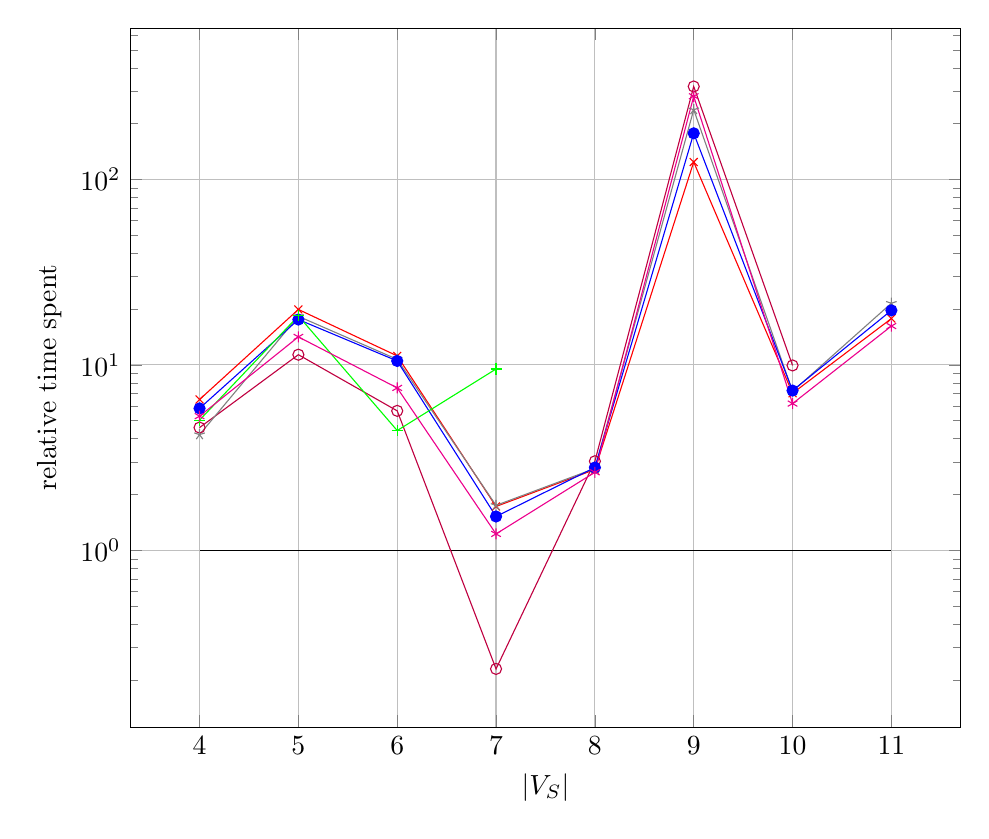
\begin{tikzpicture}
    \begin{axis}[
        xlabel=$|V_S|$,
        ylabel=relative time spent,
        ymode=log,
        legend style={at={(0.9,0.1)},anchor=south east},
        width=\textwidth,
		y tick label style={/pgf/number format/sci},
        ymajorgrids,
        xmajorgrids,		
    ]
\addplot [mark=none, black] plot coordinates {
        (4,1) (11, 1)};

%    \node[] at (axis cs: 9,1.1) {Awaiting test results (CAES server)};


\addplot[
        mark=x,
        red,
    ] plot coordinates {
        (4,6.506721650403205)
        (5,19.909363887543122)
        (6,11.177297154921606)
        (7,1.724519080351556)
        (8,2.7285266745194945)
        (9,124.16181657015836)
        (10,7.031445004959032)
        (11,17.775679517060333)
};
%    \addlegendentry{DFS}


\addplot[
        mark=o,
        purple,
    ] plot coordinates {
        (4,4.591167743768188)
        (5,11.350912752822408)
        (6,5.65138232112045)
        (7,0.22941169442122966)
        (8,3.022521866223289)
        (9,317.2200653821222)
        (10,9.933613641908536)
};
%    \addlegendentry{GDFS O IP}


\addplot[
        mark=star,
        gray,
    ] plot coordinates {
        (4,4.207074680497982)
        (5,18.284434265485746)
        (6,10.709129649746266)
        (7,1.7482843191894677)
        (8,2.7628381393187915)
        (9,237.7691906661526)
        (10,7.2060962391545695)
        (11,21.510504634766995)
};
%    \addlegendentry{GDFS C}


\addplot[
        mark=*,
        blue,
    ] plot coordinates {
        (4,5.828596980071678)
        (5,17.56552393240703)
        (6,10.500132546594331)
        (7,1.5222497146218434)
        (8,2.7964449321329083)
        (9,177.3520386845159)
        (10,7.269881235493629)
        (11,19.678511605024486)
};
%    \addlegendentry{K-Path}
\addplot[
        mark=+,
        green,
    ] plot coordinates {
        (4,5.034988757242889)
        (5,18.379644895855858)
        (6,4.42492369951899)
        (7,9.504410596005838)
};
%    \addlegendentry{CP}


\addplot[
        mark=asterisk,
        magenta,
    ] plot coordinates {
        (4,5.291688590357283)
        (5,14.16162037925404)
        (6,7.513687814173463)
        (7,1.2262338445252592)
        (8,2.635480706053349)
        (9,280.95194542270235)
        (10,6.186575229718758)
        (11,16.197435578006964)
};
%    \addlegendentry{GDFS A IP}


	
    \end{axis}
    \end{tikzpicture}
\caption{$|V_T|=3*|V_S|$ (cached)}

\end{subfigure}
}
\newline
\resizebox{0.28\textheight}{!}{
\begin{subfigure} {0.5\linewidth}

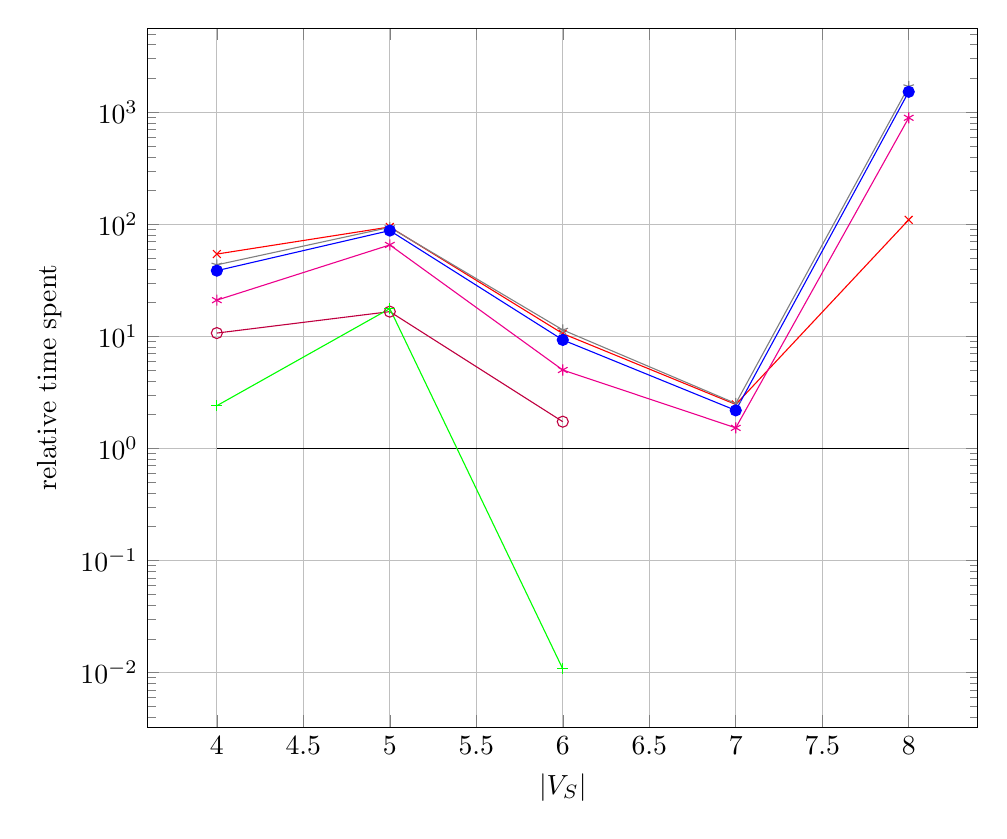
\begin{tikzpicture}
    \begin{axis}[
        xlabel=$|V_S|$,
        ylabel=relative time spent,
        ymode=log,
        legend style={at={(0.9,0.1)},anchor=south east},
        width=\textwidth,
		y tick label style={/pgf/number format/sci},
        ymajorgrids,
        xmajorgrids,		
    ]
\addplot [mark=none, black] plot coordinates {
        (4,1) (8, 1)};


%    \node[] at (axis cs: 9,1.1) {Awaiting test results (CAES server)};


\addplot[
        mark=x,
        red,
    ] plot coordinates {
        (4,54.244632157024924)
        (5,94.67410125160248)
        (6,10.579022919199833)
        (7,2.467884806621709)
        (8,109.61796961417762)
};
%    \addlegendentry{DFS}
\addplot[
        mark=o,
        purple,
    ] plot coordinates {
        (4,10.696848569213739)
        (5,16.61647755676102)
        (6,1.7322365504694384)
};
%    \addlegendentry{GDFS O IP}


\addplot[
        mark=star,
        gray,
    ] plot coordinates {
        (4,43.465930808198564)
        (5,93.92255198591933)
        (6,11.412954212374762)
        (7,2.518522472050785)
        (8,1697.6384316902834)
};
%    \addlegendentry{GDFS C}


\addplot[
        mark=*,
        blue,
    ] plot coordinates {
        (4,38.576420798557756)
        (5,87.89857301021381)
        (6,9.292817526299109)
        (7,2.183982399647286)
        (8,1521.5144724464335)
};
%    \addlegendentry{K-Path}


\addplot[
        mark=+,
        green,
    ] plot coordinates {
        (4,2.4051156279390042)
        (5,17.69226975418839)
        (6,0.01077006183520568)
};
%    \addlegendentry{CP}


\addplot[
        mark=asterisk,
        magenta,
    ] plot coordinates {
        (4,21.03540301694324)
        (5,65.43192659713577)
        (6,5.008411731723122)
        (7,1.525357905120218)
        (8,892.0214429471364)
};
%    \addlegendentry{GDFS A IP}


	
    \end{axis}
    \end{tikzpicture}
\caption{$|V_T|=5*|V_S|$ (no caching)}

\end{subfigure}
}
\resizebox{0.28\textheight}{!}{
\begin{subfigure} {0.5\linewidth}

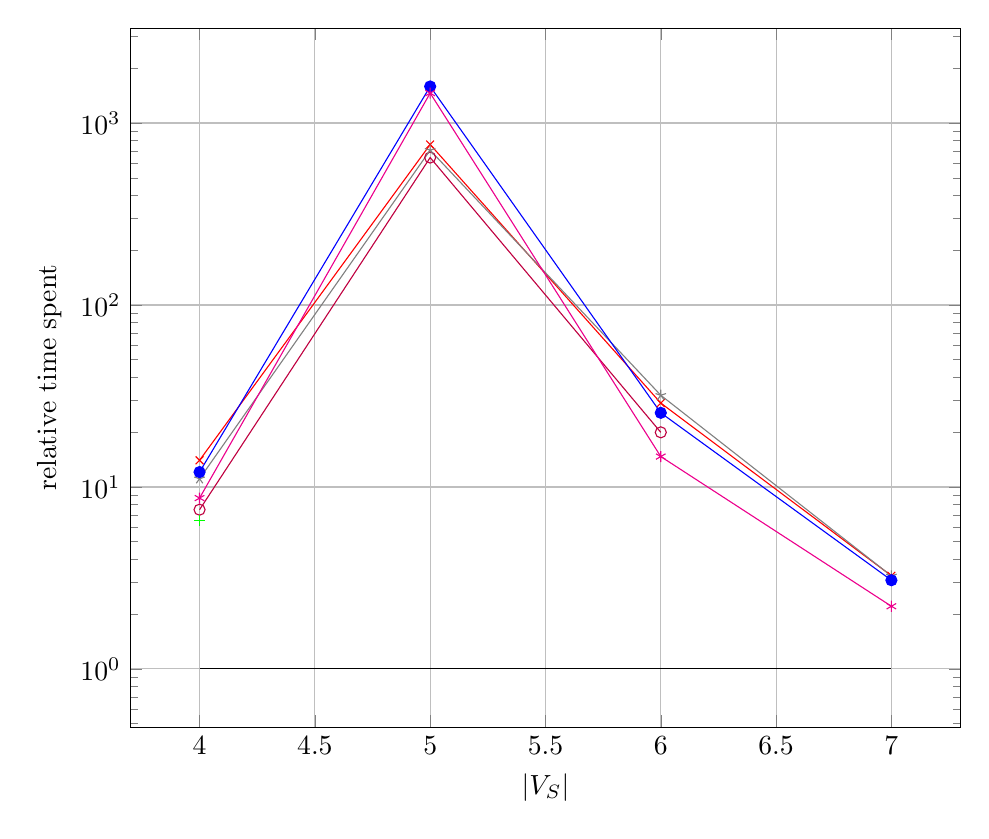
\begin{tikzpicture}
    \begin{axis}[
        xlabel=$|V_S|$,
        ylabel=relative time spent,
        ymode=log,
        legend style={at={(0.9,0.1)},anchor=south east},
        width=\textwidth,
		y tick label style={/pgf/number format/sci},
        ymajorgrids,
        xmajorgrids,		
    ]
\addplot [mark=none, black] plot coordinates {
        (4,1) (7, 1)};

%    \node[] at (axis cs: 9,1.1) {Awaiting test results (CAES server)};


\addplot[
        mark=x,
        red,
    ] plot coordinates {
        (4,14.014442936425434)
        (5,762.1422676420387)
        (6,28.909066998258137)
        (7,3.2500045042967773)
};
%    \addlegendentry{DFS}


\addplot[
        mark=o,
        purple,
    ] plot coordinates {
        (4,7.500984134455194)
        (5,645.9950612990576)
        (6,19.964026565489586)
};
%    \addlegendentry{GDFS O IP}


\addplot[
        mark=star,
        gray,
    ] plot coordinates {
        (4,11.095723351464535)
        (5,709.242281166574)
        (6,31.912378240077096)
        (7,3.2455637430524833)
};
%    \addlegendentry{GDFS C}


\addplot[
        mark=*,
        blue,
    ] plot coordinates {
        (4,12.071862186804472)
        (5,1588.441230780402)
        (6,25.547353262290816)
        (7,3.0715704037334586)
};
%    \addlegendentry{K-Path}
\addplot[
        mark=+,
        green,
    ] plot coordinates {
        (4,6.572698252534947)
};
%    \addlegendentry{CP}


\addplot[
        mark=asterisk,
        magenta,
    ] plot coordinates {
        (4,8.686387496374607)
        (5,1460.2833829253511)
        (6,14.692897155453814)
        (7,2.2099232478638378)
};
%    \addlegendentry{GDFS A IP}


	
    \end{axis}
    \end{tikzpicture}
\caption{$|V_T|=5*|V_S|$ (cached)}

\end{subfigure}
}

\caption{Performance of our algorithm with the distance based target graph vertex order relative to the performance of the algorithm with the degree-based target graph vertex order. ``refuse longer paths" and contraction are disabled and we use no pruning. Data points above the black reference line denote that this ordering introduces more delay, and data points below the reference line denote that this ordering saves time. Note the logarithmic y-axis.}		
\label{fig:DistanceVersusDegree}
\end{figure}




\begin{figure}
\begin{subfigure}{.5\linewidth}
\centering

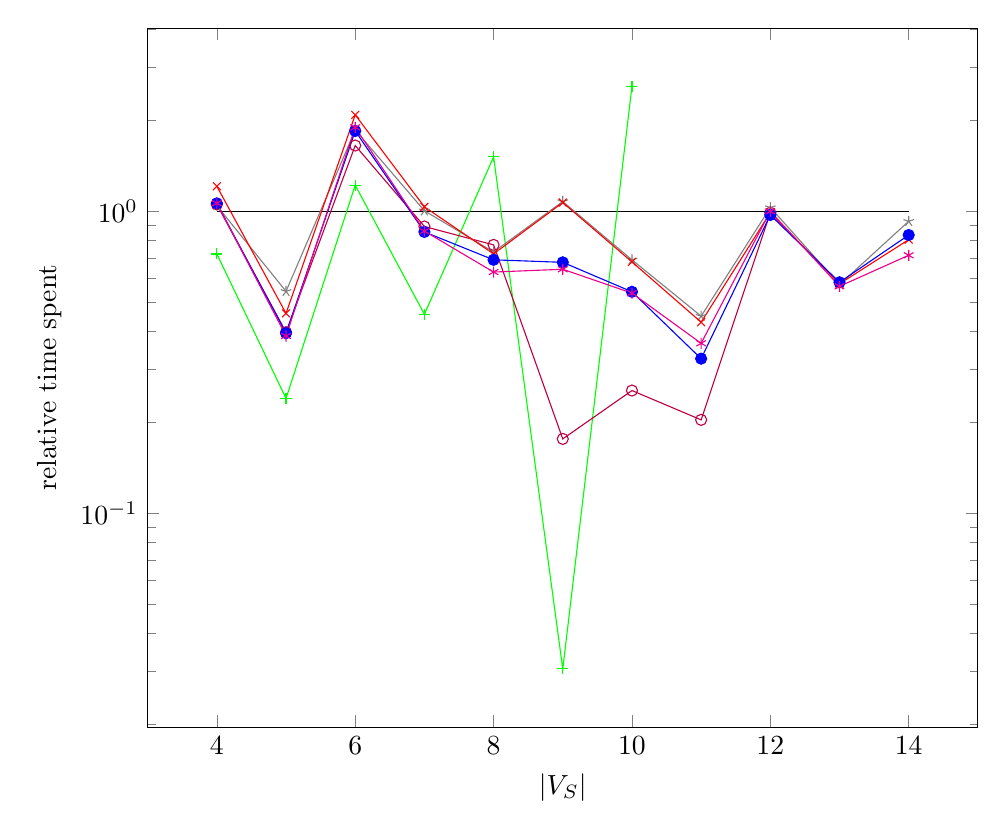
\begin{tikzpicture}
    \begin{axis}[
        xlabel=$|V_S|$,
        ylabel=relative time spent,
        ymode=log,
        legend style={at={(0.9,0.1)},anchor=south east},
        width=\textwidth,
		y tick label style={/pgf/number format/sci},
    ]


\addplot [mark=none, black] plot coordinates {
        (4,1) (14, 1)};
%\addlegendentry{No contraction}

\addplot[
        mark=+,
        green,
    ] plot coordinates {
        (4,0.7216233008103387)
        (5,0.23979959256395095)
        (6,1.219055373815801)
        (7,0.45549808099886696)
        (8,1.5129803175671477)
        (9,0.030491817239336187)
        (10,2.587109386205813)
};
%    \addlegendentry{CP}

\addplot[
        mark=o,
        purple,
    ] plot coordinates {
        (4,1.0524711376958586)
        (5,0.397430142997267)
        (6,1.649483210945216)
        (7,0.8895236575282935)
        (8,0.7731988158571639)
        (9,0.17613609063915775)
        (10,0.25469552245651866)
        (11,0.20364401173813004)
        (12,0.9888612062339083)
};
%    \addlegendentry{GDFS O IP}

\addplot[
        mark=star,
        gray,
    ] plot coordinates {
        (4,1.0424825365257937)
        (5,0.5426295402334718)
        (6,1.855682646836014)
        (7,1.0030303685825734)
        (8,0.732541042585068)
        (9,1.0760282051348324)
        (10,0.6898563436739937)
        (11,0.4490497012282625)
        (12,1.0279132116341756)
        (13,0.5714085857541255)
        (14,0.9256163980737115)
};
%    \addlegendentry{GDFS C}

\addplot[
        mark=x,
        red,
    ] plot coordinates {
        (4,1.208819655001192)
        (5,0.4586488473969574)
        (6,2.083424951258273)
        (7,1.0333509881095415)
        (8,0.7217323256161471)
        (9,1.067791165771744)
        (10,0.6792053743658721)
        (11,0.42883471023577835)
        (12,0.9888018890272706)
        (13,0.5747328589505348)
        (14,0.8046705504898993)
};
%    \addlegendentry{DFS}

\addplot[
        mark=*,
        blue,
    ] plot coordinates {
        (4,1.0612749917741098)
        (5,0.3945236842140588)
        (6,1.8429590288918432)
        (7,0.8535961630308873)
        (8,0.6899304068674341)
        (9,0.6769900545914925)
        (10,0.5407198063482145)
        (11,0.3247299866242016)
        (12,0.9713817184344807)
        (13,0.5813925975914811)
        (14,0.8336248540971392)
};
%    \addlegendentry{K-Path}

\addplot[
        mark=asterisk,
        magenta,
    ] plot coordinates {
        (4,1.0622283595408073)
        (5,0.38615187683924507)
        (6,1.894044220650229)
        (7,0.8590163375653131)
        (8,0.6286080587791637)
        (9,0.6420560054284833)
        (10,0.5352470679476732)
        (11,0.36511431500997044)
        (12,0.9985286266608072)
        (13,0.5638366376132966)
        (14,0.7142330269028185)
};
%    \addlegendentry{GDFS A IP}




    \end{axis}
    \end{tikzpicture}


\caption{$|V_T|=1\frac{1}{2}|V_S|$}
\end{subfigure}%
\begin{subfigure}{.5\linewidth}
\centering

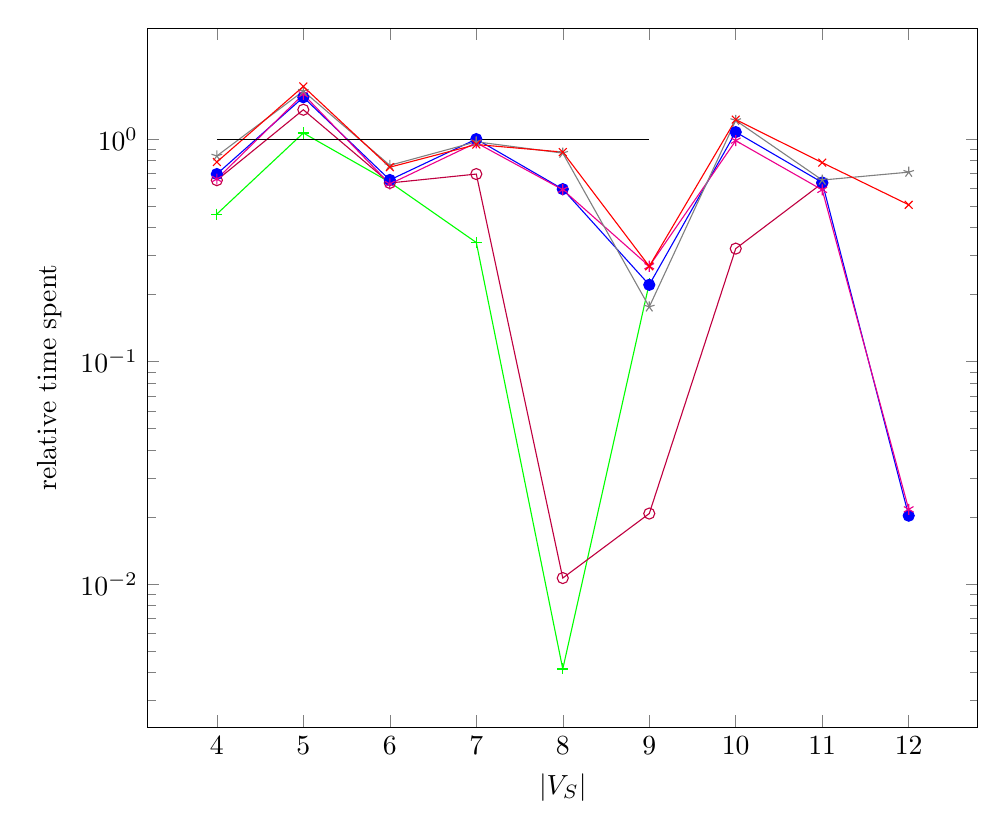
\begin{tikzpicture}
    \begin{axis}[
        xlabel=$|V_S|$,
        ylabel=relative time spent,
        ymode=log,
        legend style={at={(0.9,0.1)},anchor=south east},
        width=\textwidth,
		y tick label style={/pgf/number format/sci},
    ]

\addplot[
        mark=+,
        green,
    ] plot coordinates {
        (4,0.4603454215293834)
        (5,1.0650216337194074)
        (6,0.6402609902641055)
        (7,0.3429545951232229)
        (8,0.004156976828625529)
        (9,0.22489814118245785)
};
 %   \addlegendentry{CP}
    
    \addplot[
        mark=o,
        purple,
    ] plot coordinates {
        (4,0.6536194606761304)
        (5,1.3546625727069868)
        (6,0.6349737425008939)
        (7,0.6963677891889153)
        (8,0.010649285020911963)
        (9,0.02075639387474258)
        (10,0.3219692946843138)
        (11,0.6331864854788115)
};
 %   \addlegendentry{GDFS O IP}

\addplot[
        mark=*,
        blue,
    ] plot coordinates {
        (4,0.6964763815520504)
        (5,1.5418767352722276)
        (6,0.655132639298351)
        (7,0.9999288333397025)
        (8,0.5958121258705841)
        (9,0.22131003316388181)
        (10,1.0751746486592535)
        (11,0.6382538165641153)
        (12,0.02029968985193284)
};
  %  \addlegendentry{K-Path}
    
    
    \addplot[
        mark=asterisk,
        magenta,
    ] plot coordinates {
        (4,0.6613792478641376)
        (5,1.5903154443877043)
        (6,0.6283278818175081)
        (7,0.9629244885375634)
        (8,0.5921232096268492)
        (9,0.2682914762370498)
        (10,0.9835719984313271)
        (11,0.5912237044773625)
        (12,0.02168235616079701)
};
  %  \addlegendentry{GDFS A IP}
    
    
    \addplot[
        mark=star,
        gray,
    ] plot coordinates {
        (4,0.8400238494760311)
        (5,1.6432913297339495)
        (6,0.7623783834679656)
        (7,0.9724418464068187)
        (8,0.8649452249859358)
        (9,0.17617155505832582)
        (10,1.212740370430325)
        (11,0.6545125286561274)
        (12,0.7102484891877338)
};
 %   \addlegendentry{GDFS C}
    
    \addplot[
        mark=x,
        red,
    ] plot coordinates {
        (4,0.7890817980923504)
        (5,1.7236983707312352)
        (6,0.7476536478460998)
        (7,0.9454835701186506)
        (8,0.8743040069418077)
        (9,0.2682189465805335)
        (10,1.2231897365346933)
        (11,0.7838936485791846)
        (12,0.5066592201432429)
};
%    \addlegendentry{DFS}

\addplot [mark=none, black] plot coordinates {
        (4,1) (9, 1)};
%\addlegendentry{No contraction}


	
    \end{axis}
    \end{tikzpicture}

\caption{$|V_T|=3|V_S|$}
\end{subfigure}\\[1ex]
\begin{subfigure}{0.5\linewidth}
\centering

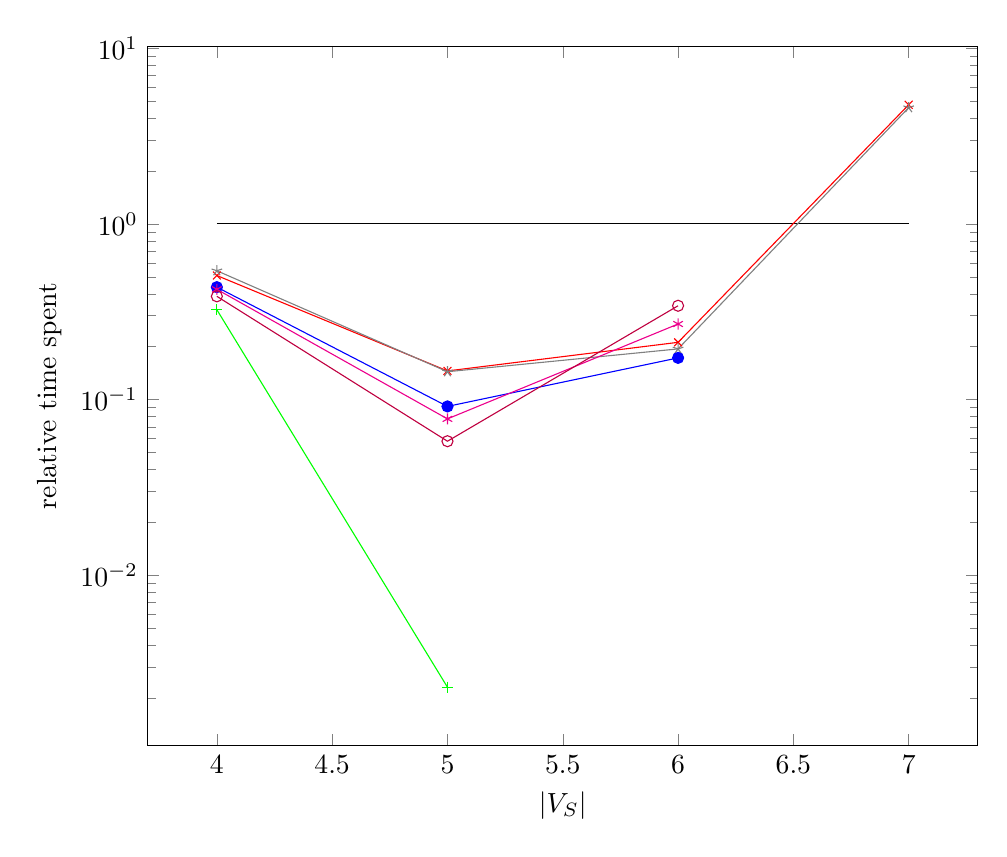
\begin{tikzpicture}
    \begin{axis}[
        xlabel=$|V_S|$,
        ylabel=relative time spent,
        ymode=log,
        legend style={at={(0.9,0.1)},anchor=south east},
        width=\textwidth,
		y tick label style={/pgf/number format/sci},
    ]


\addplot [mark=none, black] plot coordinates {
        (4,1) (7, 1)};
%\addlegendentry{No contraction}
\addplot[
        mark=+,
        green,
    ] plot coordinates {
        (4,0.3247986778213492)
        (5,0.0023085173636887735)
};
%    \addlegendentry{CP}


\addplot[
        mark=x,
        red,
    ] plot coordinates {
        (4,0.5083088516623958)
        (5,0.14560631066960938)
        (6,0.21180693936992814)
        (7,4.763971312568752)
};
 %   \addlegendentry{DFS}


\addplot[
        mark=star,
        gray,
    ] plot coordinates {
        (4,0.5412364762939754)
        (5,0.14410181776854825)
        (6,0.19432561438404647)
        (7,4.587173792533694)
};
%    \addlegendentry{GDFS C}


\addplot[
        mark=*,
        blue,
    ] plot coordinates {
        (4,0.43647426849988535)
        (5,0.09146773493441722)
        (6,0.17275569282732595)
};
 %   \addlegendentry{K-Path}


\addplot[
        mark=asterisk,
        magenta,
    ] plot coordinates {
        (4,0.4241962520645475)
        (5,0.07767539614505417)
        (6,0.26930850582566696)
};
 %   \addlegendentry{GDFS A IP}


\addplot[
        mark=o,
        purple,
    ] plot coordinates {
        (4,0.38706533483340066)
        (5,0.05797333316929685)
        (6,0.34203860563242006)
};
%    \addlegendentry{GDFS O IP}

	
	
    \end{axis}
    \end{tikzpicture}

\caption{$|V_T|=5|V_S|$}
\end{subfigure}
\begin{subfigure} {0.5\linewidth}
\centering

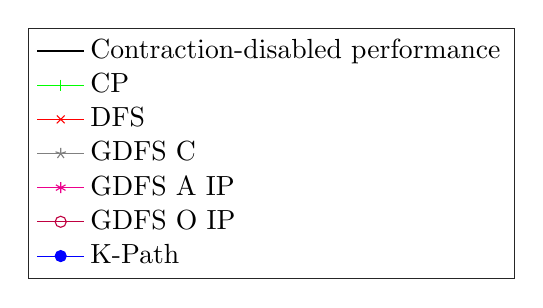
\begin{tikzpicture} 
    \begin{axis}[%
    hide axis,
    xmin=10,
    xmax=50,
    ymin=0,
    ymax=0.4,
    legend style={draw=white!15!black,legend cell align=left}
    ]
	\addlegendimage{black}
    \addlegendentry{Contraction-disabled performance}; 
     
    \addlegendimage{green, mark=+}
    \addlegendentry{CP};
    
    \addlegendimage{red, mark=x}
    \addlegendentry{DFS};
    
    \addlegendimage{gray, mark=star}
    \addlegendentry{GDFS C};
    
    \addlegendimage{magenta, mark=asterisk}
    \addlegendentry{GDFS A IP};
    
    \addlegendimage{purple, mark=o}
    \addlegendentry{GDFS O IP};
    
    \addlegendimage{blue, mark=*}
    \addlegendentry{K-Path};
    
    \end{axis}
\end{tikzpicture}

\end{subfigure}

\caption{Performance of our algorithm with the degree-based target graph vertex order relative to the performance of the algorithm with a random target graph vertex order. We avoid unnecessarily long paths, do not perform contraction and use no pruning. Data points above the black reference line denote the degree-based ordering introduces more delay, and data points below the reference line denote that it saves time. Note the logarithmic y-axis.}	
\label{fig:greatestDegreeVersusRandom}
\end{figure}



\begin{figure}
\begin{subfigure}{.5\linewidth}
\centering

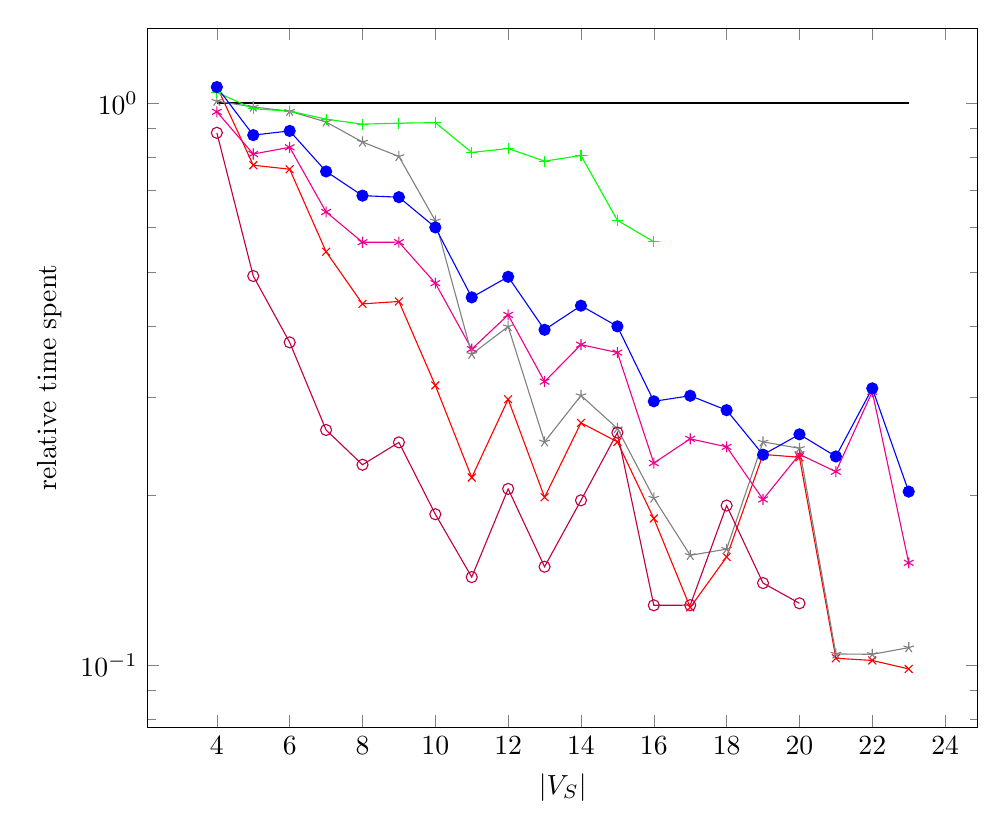
\begin{tikzpicture}
    \begin{axis}[
        xlabel=$|V_S|$,
        ylabel=relative time spent,
        ymode=log,
        legend style={at={(0.9,0.1)},anchor=south east},
        width=\textwidth,
		y tick label style={/pgf/number format/sci},
    ]


\addplot [mark=none, black] plot coordinates {
        (4,1) (23, 1)};
%\addlegendentry{No contraction}

	
   	\addplot[
        mark=x,
        red,
    ] plot coordinates {
    (4,1.0701376596978578)
        (5,0.7750483833840601)
        (6,0.7625239659727396)
        (7,0.5435907248272545)
        (8,0.43905625641231655)
        (9,0.44333498504649627)
        (10,0.31427736006275914)
        (11,0.21549418093434788)
        (12,0.29700850327105366)
        (13,0.19875803647232598)
        (14,0.26960460127846947)
        (15,0.24943654671207566)
        (16,0.1822160520770154)
        (17,0.12652580040513978)
        (18,0.15557887314603722)
        (19,0.23690016515325316)
        (20,0.23413010848141239)
        (21,0.10274440066614124)
        (22,0.1018143796654711)
        (23,0.09833948238303787)
};
%    \addlegendentry{DFS}

\addplot[
        mark=asterisk,
        magenta,
    ] plot coordinates {
        (4,0.9646835529917239)
        (5,0.8113643330208755)
        (6,0.8340623913309159)
        (7,0.6399015712888031)
        (8,0.5651878881557018)
        (9,0.5653315538963386)
        (10,0.47794089388172367)
        (11,0.3647432871506055)
        (12,0.4196279793254562)
        (13,0.31920174684238656)
        (14,0.3714797511403636)
        (15,0.35966164286125674)
        (16,0.2286295557311787)
        (17,0.25250106787609233)
        (18,0.24436238655507947)
        (19,0.19700769848171182)
        (20,0.23697864076629702)
        (21,0.2206956999692248)
        (22,0.3062630315305542)
        (23,0.15194030658042346)
};
%    \addlegendentry{GDFS A IP}

\addplot[
        mark=star,
        gray,
    ] plot coordinates {
        (4,1.0076928820459565)
        (5,0.983901080688342)
        (6,0.9669262144955426)
        (7,0.9252245633448803)
        (8,0.8522498237398553)
        (9,0.8032759861174249)
        (10,0.6171724435688729)
        (11,0.35723830908397847)
        (12,0.4000599943535533)
        (13,0.24939686313601822)
        (14,0.3015786625876812)
        (15,0.2634252154093511)
        (16,0.19816461150852743)
        (17,0.15666932104640147)
        (18,0.16070461860726504)
        (19,0.2493749238156936)
        (20,0.24288582897080782)
        (21,0.10457106920534778)
        (22,0.10441999655858641)
        (23,0.10730037259146949)
};
%    \addlegendentry{GDFS C}

\addplot[
        mark=o,
        purple,
    ] plot coordinates {
        (4,0.8850973682092008)
        (5,0.49211719526852293)
        (6,0.3749857639782973)
        (7,0.26185344137719707)
        (8,0.22707613716934089)
        (9,0.24886610684918653)
        (10,0.18538190648139338)
        (11,0.143287178899486)
        (12,0.20567173874574307)
        (13,0.1494998841435096)
        (14,0.1962904826921925)
        (15,0.25901877438054843)
        (16,0.12764073117929187)
        (17,0.1277078372348921)
        (18,0.19211906685956734)
        (19,0.13981954023222753)
        (20,0.12868526509582714)
};
%    \addlegendentry{GDFS O IP}

\addplot[
        mark=+,
        green,
    ] plot coordinates {
        (4,1.0447200482417789)
        (5,0.9768014047219801)
        (6,0.9674489096177588)
        (7,0.9359261518821227)
        (8,0.9170755875946195)
        (9,0.9208456200850942)
        (10,0.9226483399970833)
        (11,0.8167296172561879)
        (12,0.8299040306597638)
        (13,0.7882084677764385)
        (14,0.8065343267082437)
        (15,0.6182293453860566)
        (16,0.5664050892049144)
};
%    \addlegendentry{CP}

\addplot[
        mark=*,
        blue,
    ] plot coordinates {
     (4,1.067574077798301)
        (5,0.8767234058268033)
        (6,0.8920189758885858)
        (7,0.7554709717371)
        (8,0.6841141477377559)
        (9,0.6798868705510517)
        (10,0.6006702804910036)
        (11,0.4508897423728995)
        (12,0.49054030937361914)
        (13,0.3948424128676263)
        (14,0.4358083432482373)
        (15,0.40033987136573546)
        (16,0.2944817051689707)
        (17,0.3012804658022599)
        (18,0.28397895980322047)
        (19,0.23660584413000785)
        (20,0.257186007511192)
        (21,0.2349170834392937)
        (22,0.31059677707523903)
        (23,0.2033838178427883)
};
%    \addlegendentry{K-Path}
   

    \end{axis}
    \end{tikzpicture}


\caption{$|V_T|=1\frac{1}{2}|V_S|$}
\end{subfigure}%
\begin{subfigure}{.5\linewidth}
\centering

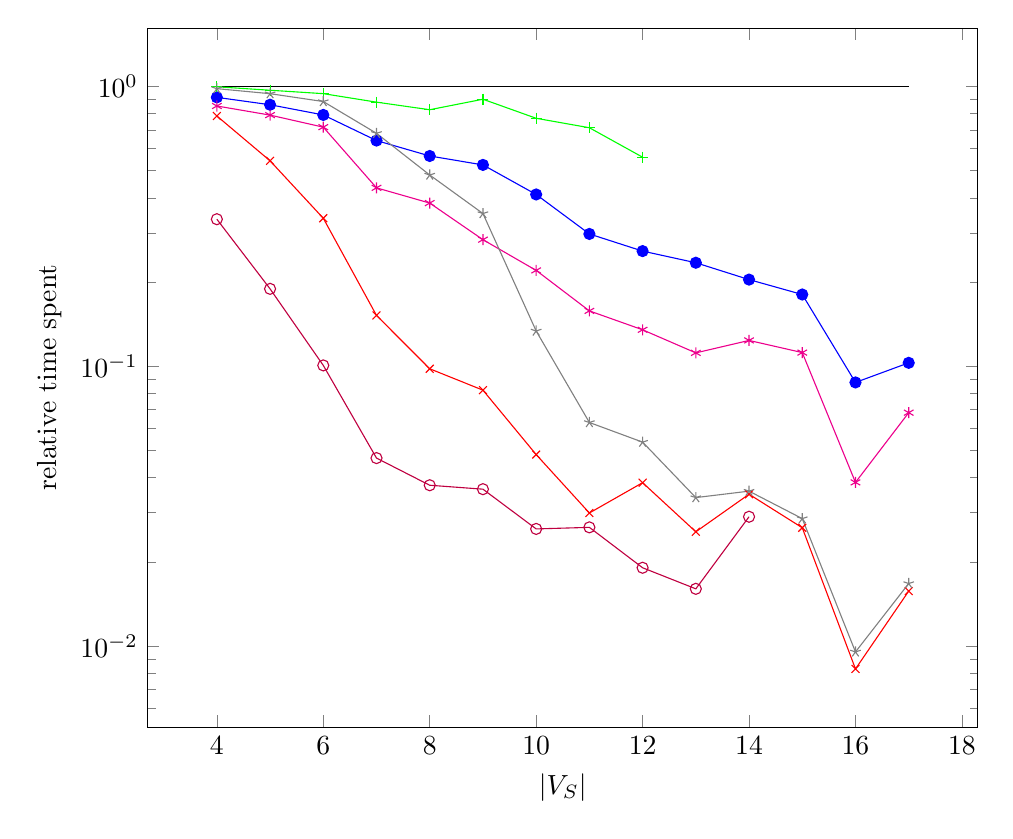
\begin{tikzpicture}
    \begin{axis}[
        xlabel=$|V_S|$,
        ylabel=relative time spent,
        ymode=log,
        legend style={at={(0.9,0.1)},anchor=south east},
        width=\textwidth,
		y tick label style={/pgf/number format/sci},
    ]


\addplot [mark=none, black] plot coordinates {
        (4,1) (17, 1)};
%\addlegendentry{No contraction}

	
\addplot[
        mark=*,
        blue,
    ] plot coordinates {
        (4,0.9144351873245234)
        (5,0.8604827367991432)
        (6,0.7913807944471791)
        (7,0.6408747361080422)
        (8,0.5644869931387801)
        (9,0.5244957804593064)
        (10,0.41127045927825046)
        (11,0.29721708517427003)
        (12,0.25807846072204743)
        (13,0.23450003716530787)
        (14,0.20415508777162117)
        (15,0.1806016795323983)
        (16,0.08759221597847955)
        (17,0.1029272468937503)
 
};
 %   \addlegendentry{K-Path}
    
    
    
    \addplot[
        mark=asterisk,
        magenta,
    ] plot coordinates {
        (4,0.8517306816100106)
        (5,0.7903396576378922)
        (6,0.715605937049185)
        (7,0.43437312425655195)
        (8,0.3831879607610557)
        (9,0.28351535934948463)
        (10,0.22018179650022743)
        (11,0.15781373311519534)
        (12,0.13507446584999497)
        (13,0.11170957349041666)
        (14,0.12375046702003706)
        (15,0.11197654989350668)
        (16,0.03848467373571145)
        (17,0.06830118707399156)
   
};
 %   \addlegendentry{GDFS A IP}
    
    
    \addplot[
        mark=x,
        red,
    ] plot coordinates {
        (4,0.7846872619727697)
        (5,0.5424712735363988)
        (6,0.3382315124928066)
        (7,0.15200192583513225)
        (8,0.09801750480507616)
        (9,0.08219886549722584)
        (10,0.04838061481784399)
        (11,0.0299220609181214)
        (12,0.03839698220605832)
        (13,0.025633258543015524)
        (14,0.034913185288842526)
        (15,0.026500220293965936)
        (16,0.008292853704258583)
        (17,0.01573584213744253)
      
};
%    \addlegendentry{DFS}

\addplot[
        mark=+,
        green,
    ] plot coordinates {
        (4,0.9973998175073646)
        (5,0.9695932261369062)
        (6,0.9426984145150554)
        (7,0.8790360004733055)
        (8,0.8258952335172475)
        (9,0.9003838932139886)
        (10,0.7698527105174667)
        (11,0.7122224617463608)
        (12,0.5588810419114151)
     
};
%    \addlegendentry{CP}

\addplot[
        mark=o,
        purple,
    ] plot coordinates {
        (4,0.33554458139095233)
        (5,0.18918210118040157)
        (6,0.1007740374152106)
        (7,0.04700465229827888)
        (8,0.03759650462559647)
        (9,0.036396221646248145)
        (10,0.02624491328700947)
        (11,0.02658394145808671)
        (12,0.019067253573874218)
        (13,0.016032335955180207)
        (14,0.029010454773618948)
     
};
%    \addlegendentry{GDFS O IP}

\addplot[
        mark=star,
        gray,
    ] plot coordinates {
        (4,0.9823157213858835)
        (5,0.9423930396188176)
        (6,0.8834397867884509)
        (7,0.6802397523203553)
        (8,0.4827313559711965)
        (9,0.35157298039088664)
        (10,0.13375480538418397)
        (11,0.06300868845254717)
        (12,0.05360184520525508)
        (13,0.03396322326203567)
        (14,0.035813414894332325)
        (15,0.02857019872219001)
        (16,0.00953880632335426)
        (17,0.016748489489447828)
      
};
%    \addlegendentry{GDFS C}


    \end{axis}
    \end{tikzpicture}

\caption{$|V_T|=3|V_S|$}
\end{subfigure}\\[1ex]
\begin{subfigure}{0.5\linewidth}
\centering

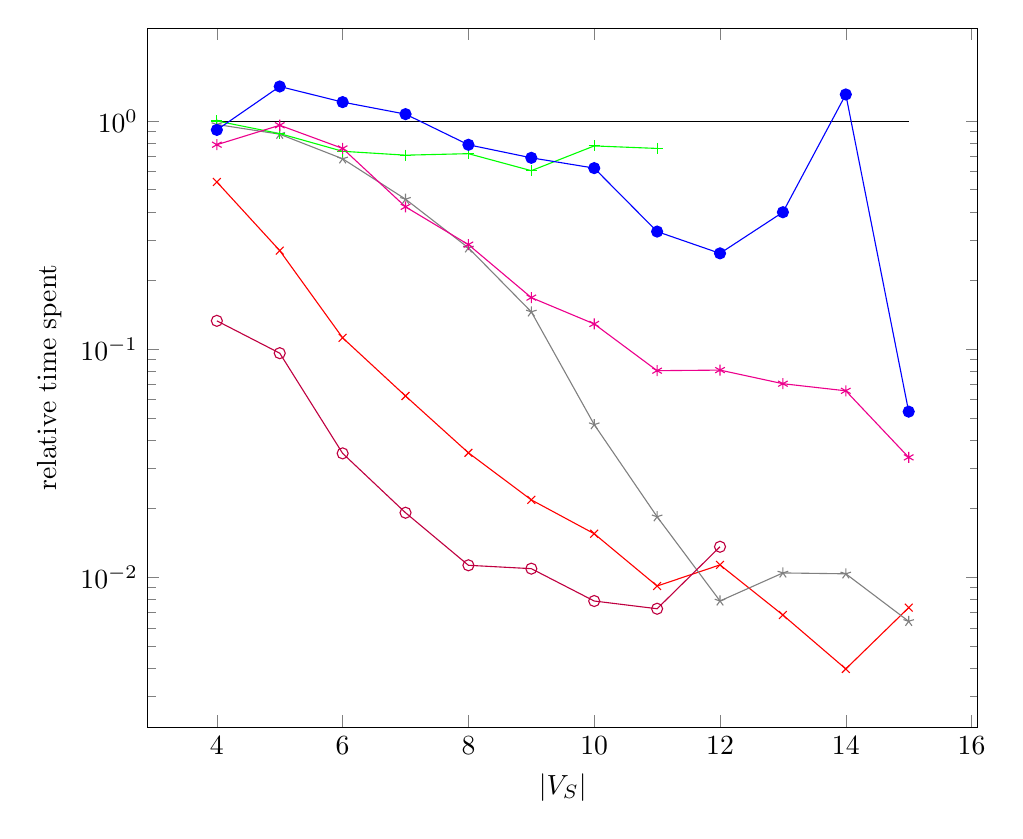
\begin{tikzpicture}
    \begin{axis}[
        xlabel=$|V_S|$,
        ylabel=relative time spent,
        ymode=log,
        legend style={at={(0.9,0.1)},anchor=south east},
        width=\textwidth,
		y tick label style={/pgf/number format/sci},
    ]


\addplot [mark=none, black] plot coordinates {
        (4,1) (15, 1)};
%\addlegendentry{No contraction}

	

\addplot[
        mark=x,
        red,
    ] plot coordinates {
        (4,0.5411179697032152)
        (5,0.2704930524379897)
        (6,0.11213082723419009)
        (7,0.06232599283874147)
        (8,0.035108158298212004)
        (9,0.021832359512569)
        (10,0.01551029778400324)
        (11,0.009148749886694655)
        (12,0.011322643138557083)
        (13,0.00682563520131426)
        (14,0.00396036408059703)
        (15,0.007353396321165447)      
};
%    \addlegendentry{DFS}

\addplot[
        mark=star,
        gray,
    ] plot coordinates {
        (4,0.9666239578598108)
        (5,0.8762877842065461)
        (6,0.683608559713269)
        (7,0.4546873986370473)
        (8,0.27810210244800715)
        (9,0.14573574757374422)
        (10,0.04669051634035179)
        (11,0.01841463663053203)
        (12,0.007868256524489591)
        (13,0.010439288181501596)
        (14,0.010347609542544794)
        (15,0.0064051732486205175)
       
};
%    \addlegendentry{GDFS C}


\addplot[
        mark=+,
        green,
    ] plot coordinates {
        (4,1.0015024125207466)
        (5,0.8816514833540374)
        (6,0.7375927572761795)
        (7,0.7090274940418195)
        (8,0.7199742258925761)
        (9,0.6062582608534516)
        (10,0.7786554757622911)
        (11,0.759062007941154)
       
};
%    \addlegendentry{CP}


\addplot[
        mark=o,
        purple,
    ] plot coordinates {
        (4,0.13311802967905184)
        (5,0.09603338861901747)
        (6,0.034918336842012156)
        (7,0.01917346709192102)
        (8,0.011276855984884832)
        (9,0.01090036189935871)
        (10,0.007862390877023315)
        (11,0.007272947391639492)
        (12,0.01359730670398279)
      
};
%    \addlegendentry{GDFS O IP}

\addplot[
        mark=asterisk,
        magenta,
    ] plot coordinates {
        (4,0.788292323592923)
        (5,0.9590318454161153)
        (6,0.7592089649215885)
        (7,0.4208192590438211)
        (8,0.2873834837908332)
        (9,0.16830317135597236)
        (10,0.12898635225142394)
        (11,0.08047180918507638)
        (12,0.0809381779051798)
        (13,0.07055502127681917)
        (14,0.06566668124638324)
        (15,0.03353747138923799)
       
};
%    \addlegendentry{GDFS A IP}


\addplot[
        mark=*,
        blue,
    ] plot coordinates {
        (4,0.9150693631849841)
        (5,1.4188871468301367)
        (6,1.211562728934971)
        (7,1.0731297341357748)
        (8,0.7875188029533118)
        (9,0.6903542117220096)
        (10,0.62219988843212)
        (11,0.3278805811742973)
        (12,0.2630839875412322)
        (13,0.3986393081117181)
        (14,1.3090500221932537)
        (15,0.053211168492635234)
      
};
%    \addlegendentry{K-Path}
	
    \end{axis}
    \end{tikzpicture}

\caption{$|V_T|=5|V_S|$}
\end{subfigure}
\begin{subfigure} {0.5\linewidth}
\centering

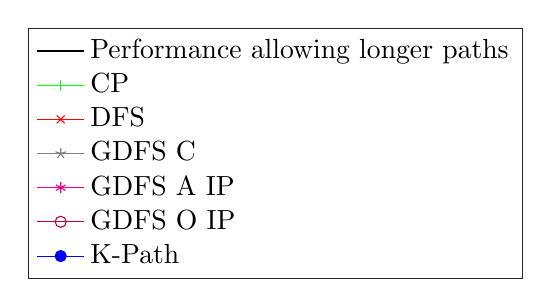
\begin{tikzpicture} 
    \begin{axis}[%
    hide axis,
    xmin=10,
    xmax=50,
    ymin=0,
    ymax=0.4,
    legend style={draw=white!15!black,legend cell align=left}
    ]
	\addlegendimage{black}
    \addlegendentry{Performance allowing longer paths}; 
     
    \addlegendimage{green, mark=+}
    \addlegendentry{CP};
    
    \addlegendimage{red, mark=x}
    \addlegendentry{DFS};
    
    \addlegendimage{gray, mark=star}
    \addlegendentry{GDFS C};
    
    \addlegendimage{magenta, mark=asterisk}
    \addlegendentry{GDFS A IP};
    
    \addlegendimage{purple, mark=o}
    \addlegendentry{GDFS O IP};
    
    \addlegendimage{blue, mark=*}
    \addlegendentry{K-Path};
    
    \end{axis}
\end{tikzpicture}

\end{subfigure}

\caption{Mean relative time consumption of \textbf{avoiding} unnecessarily long paths for subgraph homeomorphism search compared to \textbf{allowing} unneccessarily long paths for subgraph homeomorphism for different path iteration methods (no pruning or contraction, greatest constrained first / degree based orderings). For data points below the reference line refusing unnecesarily long paths saves time while for data points above it it costs extra time. We handled a maximum of 1000 test cases or 10 minutes per value of $|V_S|$ for each path iteration method.}	
\label{fig:longerpaths}
\end{figure}



\begin{figure}
\begin{subfigure}{.5\linewidth}
\centering

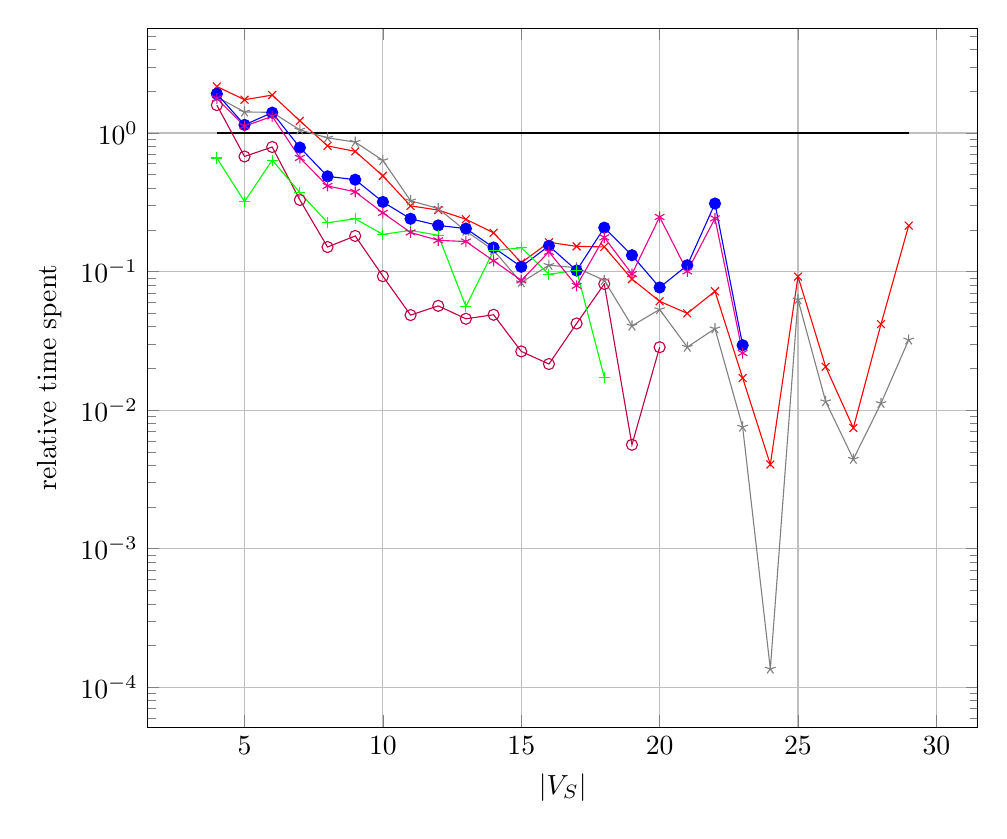
\begin{tikzpicture}
    \begin{axis}[
        xlabel=$|V_S|$,
        ylabel=relative time spent,
        ymode=log,
        legend style={at={(0.9,0.1)},anchor=south east},
        width=\textwidth,
		y tick label style={/pgf/number format/sci},
        ymajorgrids,
        xmajorgrids,		
    ]


\addplot [mark=none, black] plot coordinates {
        (4,1) (29, 1)};
%\addlegendentry{No contraction}

	\addplot[
        mark=x,
        red,
    ] plot coordinates {
        (4,2.1674128912679387)
        (5,1.7391752267555143)
        (6,1.878677825130543)
        (7,1.2249805426145646)
        (8,0.8074738280349274)
        (9,0.7370517159428939)
        (10,0.4907351225256)
        (11,0.2980550454981918)
        (12,0.2781141325880348)
        (13,0.23851995177183047)
        (14,0.19062785566800405)
        (15,0.11582540953584422)
        (16,0.16268098061869612)
        (17,0.15207093622469334)
        (18,0.15064594752021512)
        (19,0.0883792576708712)
        (20,0.06105289023128585)
        (21,0.049964135000540935)
        (22,0.0721091008374441)
        (23,0.017061614763450757)
        (24,0.004054554777087193)
        (25,0.09203806626889509)
        (26,0.020561449567552532)
        (27,0.007440675118337155)
        (28,0.0417732163780968)
        (29,0.2146145702804488)
};
%    \addlegendentry{DFS}
%    \addplot[
%        mark=x,
%        red,
%    ] plot coordinates {
%        (4,1.764570104072358)
%        (5,1.2804472403537654)
%        (6,1.1184611822085426)
%        (7,1.108193754987779)
%        (8,1.0823455102636332)
%        (9,1.3202304844536292)
%        (10,0.8766301350767352)
%        (11,2.545919815002013)
%        (12,1.0352805568707166)
%        (13,0.7348584756068407)
%        (14,0.7849914287368015)
%        (15,0.8934474568976407)
%        (16,1.6666025961560895)
%        (17,0.71724791351521)
%        (18,0.5094398225741126)
%        (19,0.8456597164761079)
%        (20,0.8045735438552715)
%        (21,0.5994679253970462)
%        (22,0.4676165222586781)
%        (23,0.10986432258137258)
%        (24,0.16189794326161777)
%        (25,0.2926263173443996)
%        (26,0.09304326805518515)
%        (27,0.042335345258718515)
%        (28,0.1650463503335008)
%        (29,0.05828381864786569)
%        (30,0.06816890123257702)
%        (31,0.014702001658170927)
%        (32,5.292125517369906E-4)
%        (33,0.48658861405918064)
%        (34,0.3275583732734606)
%        (35,54.77402524625391)
%};
%    \addlegendentry{DFS}


\addplot[
        mark=o,
        purple,
    ] plot coordinates {
        (4,1.5908169191884858)
        (5,0.6772772991230941)
        (6,0.7928925518833834)
        (7,0.32888150264765864)
        (8,0.1503793791728905)
        (9,0.18090584660161316)
        (10,0.09259090925765891)
        (11,0.04853285360340585)
        (12,0.05658374367299821)
        (13,0.045645082500291714)
        (14,0.0487971444573912)
        (15,0.026539030640982012)
        (16,0.021517848684053972)
        (17,0.04221398376336805)
        (18,0.08140898933547427)
        (19,0.00562565540553724)
        (20,0.02845179954877085)
};
%    \addlegendentry{GDFS O IP}
%\addplot[
%        mark=o,
%        purple,
%    ] plot coordinates {
%        (4,1.5465954055848148)
%        (5,0.6725582833953612)
%        (6,0.4139609581308408)
%        (7,0.36803303109353136)
%        (8,0.36527194171296373)
%        (9,0.49852548813528896)
%        (10,0.26095750210484203)
%        (11,0.21624262398197047)
%        (12,0.26820633077466083)
%        (13,0.20928330156141128)
%        (14,0.26458447534228824)
%        (15,0.2606750959815698)
%        (16,0.1519838230882713)
%        (17,0.17898927491143424)
%        (18,0.2388521888406996)
%        (19,0.4267188749902131)
%        (20,0.19982250009097213)
%        (21,0.2924664720196809)
%        (22,0.9672401778006531)
%        (23,0.027360410960048376)
%        (24,7.01509756650176E-4)
%        (25,1.2672226912043596)
%        (26,0.07078753406996308)
%        (27,0.022665056711590914)
%        (28,0.017141291453382168)
%        (29,0.24055888434774642)
%};
%    \addlegendentry{GDFS O IP}

\addplot[
        mark=star,
        gray,
    ] plot coordinates {
        (4,1.8186013757848167)
        (5,1.4197293719638007)
        (6,1.4095764617281157)
        (7,1.0529037229777707)
        (8,0.9224328522850976)
        (9,0.8606190323854189)
        (10,0.634096501164528)
        (11,0.3246356036344815)
        (12,0.28525932777239493)
        (13,0.1962056557937944)
        (14,0.14265878336059234)
        (15,0.08343495318306988)
        (16,0.11120442296044247)
        (17,0.10662648119706182)
        (18,0.08639088150368307)
        (19,0.0405823649375348)
        (20,0.053299871331840394)
        (21,0.028534152249321126)
        (22,0.038710712744670625)
        (23,0.007561487667922238)
        (24,1.356366377457008E-4)
        (25,0.0626971597400394)
        (26,0.01154512308668409)
        (27,0.004430664154583717)
        (28,0.011200653433328957)
        (29,0.0321618501659541)
};
%    \addlegendentry{GDFS C}
%    \addplot[
%        mark=star,
%        gray,
%    ] plot coordinates {
%        (4,3.0103172170217087)
%        (5,1.7008010826730877)
%        (6,1.3185993107748495)
%        (7,1.0651222844937673)
%        (8,1.0313582598355582)
%        (9,1.019847433896466)
%        (10,0.8297884970625686)
%        (11,0.7200492247409158)
%        (12,0.774512334885343)
%        (13,0.5217949486742455)
%        (14,0.5149663295021711)
%        (15,0.6077016349543982)
%        (16,1.0645804487651895)
%        (17,0.4211041381764984)
%        (18,0.2746875518186591)
%        (19,0.5346278517377602)
%        (20,0.4954917433705648)
%        (21,0.24700068708986667)
%        (22,0.2909598485628878)
%        (23,0.06682556779896554)
%        (24,0.20424256710140876)
%        (25,0.2106670647954565)
%        (26,0.035665701539059236)
%        (27,0.018999300275658104)
%        (28,0.06081303305299257)
%        (29,0.02467804462419776)
%        (30,0.06069641418283933)
%        (31,0.016093817467386362)
%        (32,7.397912089912584E-5)
%        (33,0.21324629155751507)
%        (34,0.1619915480935199)
%        (35,19.49048948725945)
%        (36,2.2331192579992156)
%};
%    \addlegendentry{GDFS C}
\addplot[
        mark=*,
        blue,
    ] plot coordinates {
        (4,1.9202928824534728)
        (5,1.1448441323276985)
        (6,1.403535875771617)
        (7,0.7854244598245812)
        (8,0.48685090235481815)
        (9,0.4603875458945484)
        (10,0.3180887280136316)
        (11,0.2405149707368394)
        (12,0.21532539772275092)
        (13,0.20439694282599416)
        (14,0.14918263315701386)
        (15,0.1083690950499177)
        (16,0.15331684928173625)
        (17,0.10175548634423026)
        (18,0.2075742872205262)
        (19,0.13122023187685616)
        (20,0.07679970343342342)
        (21,0.11103412684145902)
        (22,0.3098341880597405)
        (23,0.0294107149209991)
};
%    \addlegendentry{K-Path}
%    \addplot[
%        mark=*,
%        blue,
%    ] plot coordinates {
%        (4,1.8288452494372274)
%        (5,1.296842120241007)
%        (6,0.9012387818727957)
%        (7,0.7791122372023914)
%        (8,0.864968223092994)
%        (9,0.911626513812194)
%        (10,0.6427888393538057)
%        (11,0.7436225584218299)
%        (12,0.7549604979371962)
%        (13,0.6725293793784693)
%        (14,0.5992914625619475)
%        (15,0.8435469822917079)
%        (16,0.8272824596684006)
%        (17,0.6960713562008894)
%        (18,0.558150986832071)
%        (19,1.0626322277949884)
%        (20,0.6533296061774068)
%        (21,0.6487638110734476)
%        (22,0.2578033809500446)
%        (23,0.06052594706960124)
%        (24,0.10891268807752708)
%        (25,0.2980748961720695)
%        (26,0.05796008903103311)
%        (27,0.025237959619589523)
%        (28,0.09548260902564809)
%        (29,0.5586781624508028)
%        (30,0.5460070481456223)
%        (31,0.02831601533804662)
%        (32,7.199585374040307E-5)
%        (33,0.3599020863720135)
%        (34,0.40664654347704143)
%        (35,38.25888474739304)
%};
%    \addlegendentry{K-Path}


\addplot[
        mark=+,
        green,
    ] plot coordinates {
        (4,0.660088840101957)
        (5,0.3200751554418895)
        (6,0.6371775282011813)
        (7,0.37188567800794403)
        (8,0.22530432601006087)
        (9,0.24051735165597934)
        (10,0.18570420025909337)
        (11,0.1983771432255634)
        (12,0.18278941692499237)
        (13,0.055947078638664265)
        (14,0.1414859023192802)
        (15,0.1485911272048718)
        (16,0.09568019684337646)
        (17,0.10208470407732084)
        (18,0.01725902134774537)
};
%    \addlegendentry{CP}
%	\addplot[
%        mark=+,
%        green,
%    ] plot coordinates {
%        (4,0.8097147281048784)
%        (5,0.6974807076483973)
%        (6,0.6387765511195216)
%        (7,0.5108136511953608)
%        (8,0.6154822873000718)
%        (9,0.6178076238665242)
%        (10,0.4566675480771135)
%        (11,0.5245224457353261)
%        (12,0.43193355168311)
%        (13,0.4090918564605406)
%        (14,0.7867273649511707)
%        (15,0.4132124817740861)
%        (16,0.506998908675651)
%        (17,0.17851266569571234)
%        (18,0.016853231440474126)
%};
%    \addlegendentry{CP}

\addplot[
        mark=asterisk,
        magenta,
    ] plot coordinates {
        (4,1.7786054371985929)
        (5,1.1200606505199096)
        (6,1.319947724479513)
        (7,0.6619185199107721)
        (8,0.41497056035041624)
        (9,0.37655640061467166)
        (10,0.26516990495962656)
        (11,0.19176578151343138)
        (12,0.16806963230058247)
        (13,0.1648401627923549)
        (14,0.11964868234489424)
        (15,0.08645239633218388)
        (16,0.13865349118389622)
        (17,0.07897311226833496)
        (18,0.1765409073358474)
        (19,0.09600035877617284)
        (20,0.24782317794275846)
        (21,0.1003674889556064)
        (22,0.2420867371972601)
        (23,0.02584676124115509)
};
%    \addlegendentry{GDFS A IP}
%    \addplot[
%        mark=asterisk,
%        magenta,
%    ] plot coordinates {
%        (4,1.6604963959561405)
%        (5,1.0651196386902062)
%        (6,0.8313893618484981)
%        (7,0.6330831569415312)
%        (8,0.7025851289861612)
%        (9,0.7421127604924067)
%        (10,0.5145838783545251)
%        (11,0.555358976224104)
%        (12,0.5695323766025293)
%        (13,0.4990355735260106)
%        (14,0.448887395328494)
%        (15,0.6109556736209575)
%        (16,0.6965392752667293)
%        (17,0.4587395343719304)
%        (18,0.3984597147505228)
%        (19,0.6943628794563819)
%        (20,0.5416331210064403)
%        (21,0.47775841013253695)
%        (22,0.29035493491769016)
%        (23,0.04652391751293539)
%        (24,0.14871288585077824)
%        (25,0.1781947274150446)
%        (26,0.04490122252456785)
%        (27,0.018161498301854984)
%        (28,0.08401938735395065)
%        (29,0.8775983409797485)
%        (30,0.4542658231858391)
%        (31,0.027895820423659345)
%        (32,7.878042538378427E-5)
%        (33,0.2469129572361528)
%        (34,0.2944533235188781)
%        (35,19.738338899024424)
%};
%    \addlegendentry{GDFS A IP}

    
   

    \end{axis}
    \end{tikzpicture}


\caption{$|V_T|=1\frac{1}{2}*|V_S|$}
\end{subfigure}%
\begin{subfigure}{.5\linewidth}
\centering

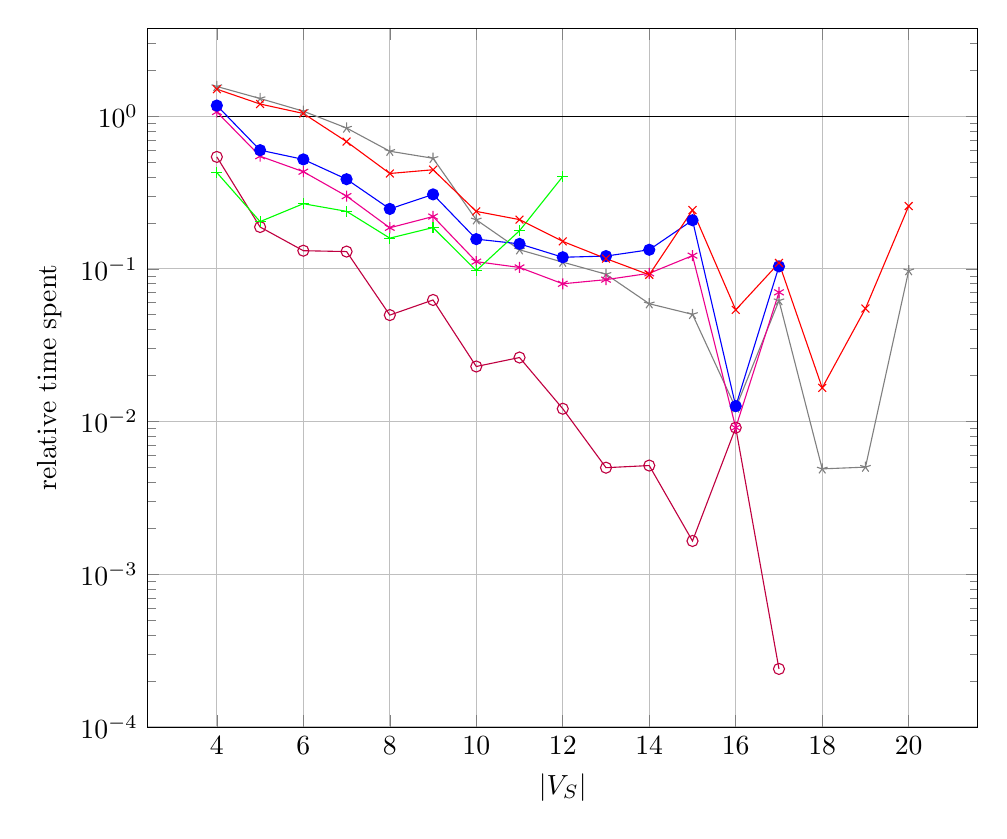
\begin{tikzpicture}
    \begin{axis}[
        xlabel=$|V_S|$,
        ylabel=relative time spent,
        ymode=log,
        legend style={at={(0.9,0.1)},anchor=south east},
        width=\textwidth,
		y tick label style={/pgf/number format/sci},
        ymajorgrids,
        xmajorgrids,		
    ]


\addplot [mark=none, black] plot coordinates {
        (4,1) (20, 1)};
%\addlegendentry{No contraction}

	
	\addplot[
        mark=o,
        purple,
    ] plot coordinates {
        (4,0.5406515860434231)
        (5,0.18785238621358155)
        (6,0.1313898693246026)
        (7,0.12968087426224423)
        (8,0.04975578786006005)
        (9,0.06250441621787829)
        (10,0.02291763153069323)
        (11,0.026239199263713514)
        (12,0.012116839676172384)
        (13,0.004980595524332248)
        (14,0.005144230579578944)
        (15,0.0016492435304128457)
        (16,0.009108127743934116)
        (17,2.39411472197788E-4)
};
%    \addlegendentry{GDFS O IP}

\addplot[
        mark=star,
        gray,
    ] plot coordinates {
        (4,1.564264576045)
        (5,1.3044268948002964)
        (6,1.0779187100450964)
        (7,0.835982515879533)
        (8,0.5891175637322107)
        (9,0.5296276854812295)
        (10,0.20943673532574508)
        (11,0.1332559624097141)
        (12,0.11055593973933432)
        (13,0.09214123221094588)
        (14,0.05906133105316621)
        (15,0.05030047639103612)
        (16,0.012261524417415466)
        (17,0.06190271276571946)
        (18,0.004891557464661643)
        (19,0.005023467236129495)
        (20,0.09721129856411416)
};
%    \addlegendentry{GDFS C}


\addplot[
        mark=asterisk,
        magenta,
    ] plot coordinates {
        (4,1.0647032384996173)
        (5,0.5464303184358585)
        (6,0.43259746830858214)
        (7,0.29933523278634744)
        (8,0.185683374814357)
        (9,0.22002307269535923)
        (10,0.11140520704714015)
        (11,0.10205941312301019)
        (12,0.0797883687267593)
        (13,0.08491982151584633)
        (14,0.09342236316366812)
        (15,0.12200531503514861)
        (16,0.009112353995585515)
        (17,0.07011738991519775)
};
%    \addlegendentry{GDFS A IP}


\addplot[
        mark=*,
        blue,
    ] plot coordinates {
        (4,1.1732008189190344)
        (5,0.5987836864801016)
        (6,0.5208779931571201)
        (7,0.3863511956599727)
        (8,0.24675777694478437)
        (9,0.3072586029941962)
        (10,0.15645774275452057)
        (11,0.14567516195730124)
        (12,0.11902720146666647)
        (13,0.12115498638742035)
        (14,0.1332611638337713)
        (15,0.20805857181266843)
        (16,0.012601727180247312)
        (17,0.10371121285669947)
};
%    \addlegendentry{K-Path}

\addplot[
        mark=+,
        green,
    ] plot coordinates {
        (4,0.4269404047456055)
        (5,0.20382248417977045)
        (6,0.2669423065984091)
        (7,0.2379083813426592)
        (8,0.15878409767837634)
        (9,0.18627099036241238)
        (10,0.09728713629116212)
        (11,0.17771427973978168)
        (12,0.4025575819836778)
};
%    \addlegendentry{CP}
	
	\addplot[
        mark=x,
        red,
    ] plot coordinates {
        (4,1.5016288184210713)
        (5,1.2006306704032468)
        (6,1.0411914932334647)
        (7,0.6807867382482929)
        (8,0.42113301579781187)
        (9,0.4454296971733875)
        (10,0.23775196252967973)
        (11,0.2099983957550243)
        (12,0.15124037808888813)
        (13,0.1166188474735059)
        (14,0.09139802130807367)
        (15,0.24260975460559725)
        (16,0.053826733086807126)
        (17,0.10922977681106211)
        (18,0.016610936461570726)
        (19,0.054963613128898324)
        (20,0.25771949929195687)
};
%    \addlegendentry{DFS}
	


%\addplot[
%        mark=x,
%        red,
%    ] plot coordinates {
%        (4,1.1732605514536567)
%        (5,1.196916188570318)
%        (6,1.1785456812485087)
%        (7,0.9954870013054639)
%        (8,3.525437510655584)
%        (9,1.4492110968852605)
%        (10,1.747381055099775)
%        (11,2.2270690506062127)
%        (12,1.2853934585525963)
%        (13,2.4238390071533145)
%        (14,1.3323905497689534)
%        (15,1.9053869795283003)
%        (16,0.48107044214796724)
%        (17,2.689105479333416)
%        (18,1.6898544382126748)
%        (19,0.9452484856043308)
%        (20,0.7898504601171549)
%        (21,0.08308472050964744)
%        (22,0.010893076925442502)
%        (23,0.1812527204673673)
%        (24,0.05728059082927839)
%        (25,5.443902225728544)
%};
%    \addlegendentry{DFS}


%\addplot[
%        mark=o,
%        purple,
%    ] plot coordinates {
%        (4,0.5520630930461605)
%        (5,0.3167780166100581)
%        (6,0.15039692039595431)
%        (7,0.24510767406414147)
%        (8,0.38213533186187054)
%        (9,0.3108804215985045)
%        (10,0.1807787773743944)
%        (11,0.3299920410160406)
%        (12,0.19012573181575232)
%        (13,0.24472040784270033)
%        (14,0.19143954341561553)
%        (15,0.6627219343829152)
%        (16,0.005733506512017317)
%        (17,3.023867931706281E-4)
%};
%    \addlegendentry{GDFS O IP}


%\addplot[
%        mark=star,
%        gray,
%    ] plot coordinates {
%        (4,2.4400816563321017)
%        (5,1.633197217665063)
%        (6,1.2185290307235452)
%        (7,0.9546648292258212)
%        (8,1.728111058353678)
%        (9,0.9769781523573012)
%        (10,0.6904942121852058)
%        (11,4.816564314417738)
%        (12,0.6783371965634181)
%        (13,4.011191995338261)
%        (14,0.7170173730516766)
%        (15,1.5965119303548203)
%        (16,0.23663227697171496)
%        (17,0.5542490660149222)
%        (18,0.3058591166536577)
%        (19,0.7018097729480665)
%        (20,0.27875622792926213)
%        (21,1.1344734954273632)
%        (22,0.028755331201753886)
%        (23,0.0777791424367319)
%};
%    \addlegendentry{GDFS C}


%\addplot[
%        mark=*,
%        blue,
%    ] plot coordinates {
%        (4,1.2419213216803755)
%        (5,0.8200821368474451)
%        (6,0.5765214516413038)
%        (7,0.565346845113148)
%        (8,1.3724712483006076)
%        (9,1.0626551826303774)
%        (10,0.8227740807006784)
%        (11,3.6735922630894127)
%        (12,1.3221239755232121)
%        (13,5.700758822957509)
%        (14,3.5989514748969498)
%        (15,1.8366783161451987)
%        (16,0.5267585376114875)
%        (17,0.8256958007787268)
%        (18,1.4987328025927649)
%        (19,0.08315275360896346)
%        (20,0.7615106824048338)
%        (21,0.2227706812823126)
%};
%    \addlegendentry{K-Path}
%	\addplot[
%        mark=+,
%        green,
%    ] plot coordinates {
%        (4,0.6251754120590031)
%        (5,0.7127354515628973)
%        (6,0.5384995648933136)
%        (7,0.4718614006762697)
%        (8,0.7587386430883546)
%        (9,0.6801119660951308)
%        (10,0.7579067651040344)
%        (11,0.6568766478712005)
%        (12,1.2358097901656984)
%};
%    \addlegendentry{CP}

%\addplot[
%        mark=asterisk,
%        magenta,
%    ] plot coordinates {
%        (4,1.0218394225281529)
%        (5,0.7182128970849538)
%        (6,0.48051752660220404)
%        (7,0.431379262711197)
%        (8,1.139769610563402)
%        (9,0.6462462777019891)
%        (10,0.4984166569477635)
%        (11,2.3191988060404114)
%        (12,0.600719665743818)
%        (13,1.9928831703649212)
%        (14,0.5997476794608112)
%        (15,2.3702852860015766)
%        (16,0.2501718737108647)
%        (17,1.963031760531809)
%        (18,0.7865261017018875)
%        (19,0.6636357792814185)
%        (20,0.4302617051584967)
%        (21,0.11666290941349455)
%        (22,0.03731454564481351)
%        (23,0.18654788991103444)
%};
%    \addlegendentry{GDFS A IP}

	
	
    \end{axis}
    \end{tikzpicture}

\caption{$|V_T|=3*|V_S|$}
\end{subfigure}\\[1ex]
\begin{subfigure}{0.5\linewidth}
\centering

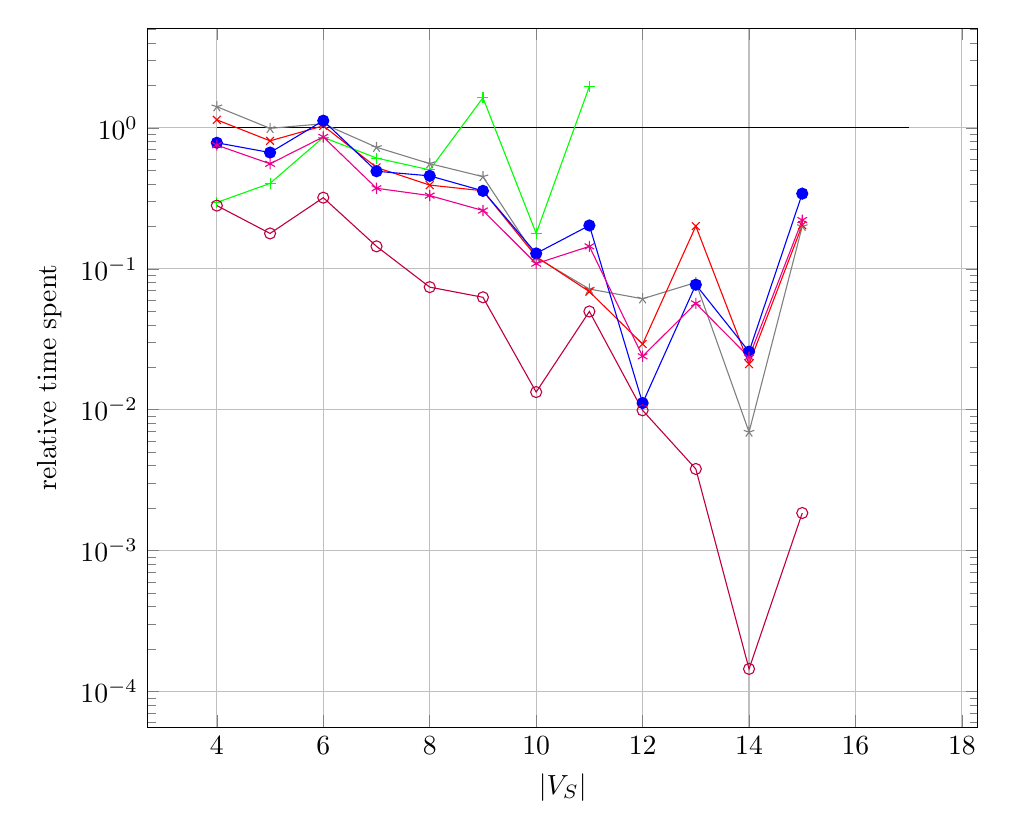
\begin{tikzpicture}
    \begin{axis}[
        xlabel=$|V_S|$,
        ylabel=relative time spent,
        ymode=log,
        legend style={at={(0.9,0.1)},anchor=south east},
        width=\textwidth,
		y tick label style={/pgf/number format/sci},
        ymajorgrids,
        xmajorgrids,		
    ]


\addplot [mark=none, black] plot coordinates {
        (4,1) (17, 1)};
%\addlegendentry{No contraction}

	\addplot[
        mark=star,
        gray,
    ] plot coordinates {
        (4,1.4150313228372156)
        (5,0.9931089780372052)
        (6,1.0711893924147513)
        (7,0.7287433844993442)
        (8,0.5580336822334304)
        (9,0.45098800643949294)
        (10,0.12035734271971275)
        (11,0.07185662459924363)
        (12,0.061270869720004735)
        (13,0.07996994856322678)
        (14,0.0069337049664659365)
        (15,0.19997291246935858)
};
%    \addlegendentry{GDFS C}

\addplot[
        mark=x,
        red,
    ] plot coordinates {
        (4,1.1414201843876104)
        (5,0.809932163821809)
        (6,1.035209481616773)
        (7,0.524271062265468)
        (8,0.39302087430090826)
        (9,0.3578043691511488)
        (10,0.12214201172912188)
        (11,0.06885304754889712)
        (12,0.029241866518748955)
        (13,0.20088131729557912)
        (14,0.02106421225202191)
        (15,0.2041959874232657)
};
%    \addlegendentry{DFS}


\addplot[
        mark=+,
        green,
    ] plot coordinates {
        (4,0.2957715422588946)
        (5,0.4039693151705631)
        (6,0.8576103567062523)
        (7,0.611136842539274)
        (8,0.5039078563666931)
        (9,1.6368759420585266)
        (10,0.17838843269084026)
        (11,1.9695600715158896)
};
%    \addlegendentry{CP}

\addplot[
        mark=*,
        blue,
    ] plot coordinates {
        (4,0.7847268248450774)
        (5,0.6687217050275467)
        (6,1.1261548415934364)
        (7,0.4925445033611991)
        (8,0.45704298044965924)
        (9,0.35742057060947313)
        (10,0.128612015175269)
        (11,0.20308934398456394)
        (12,0.011139696619114561)
        (13,0.07711180448206871)
        (14,0.025822554979476078)
        (15,0.3417612423571849)
};
%    \addlegendentry{K-Path}

\addplot[
        mark=asterisk,
        magenta,
    ] plot coordinates {
        (4,0.7547769389469375)
        (5,0.5565971887626566)
        (6,0.8633572665036556)
        (7,0.37305369668133204)
        (8,0.3309908929077787)
        (9,0.25924812346158027)
        (10,0.10882869144475564)
        (11,0.1443116551616309)
        (12,0.02393540782562589)
        (13,0.056815118476015725)
        (14,0.02359541092466829)
        (15,0.22173612580802898)
};
%    \addlegendentry{GDFS A IP}


\addplot[
        mark=o,
        purple,
    ] plot coordinates {
        (4,0.2810473555343349)
        (5,0.1782672123525788)
        (6,0.319850284994006)
        (7,0.14437026097789094)
        (8,0.07412250627959217)
        (9,0.06277787793471931)
        (10,0.013337293008856575)
        (11,0.04979135381171951)
        (12,0.009893636551485722)
        (13,0.0037954716122957726)
        (14,1.4440290497311895E-4)
        (15,0.0018470151154413993)
};
%    \addlegendentry{GDFS O IP}



%  \addplot[
%        mark=x,
%        red,
%    ] plot coordinates {
%        (4,0.8783007924961822)
%        (5,1.9866466250704127)
%        (6,46.23915298831981)
%        (7,1.9286013087935467)
%        (8,0.22144887888388298)
%        (9,0.6073880518853707)
%        (10,0.9499470941285778)
%        (11,0.3071513116204406)
%        (12,0.20181763488775617)
%        (13,0.5247142961355576)
%        (14,0.08240035713162575)
%        (15,1.3331646694970158)
%        (16,0.030153907349204312)
%        (17,0.7818188550294238)
%};
%     \addlegendentry{DFS}

%    \addplot[
%        mark=o,
%        purple,
%    ] plot coordinates {
%        (4,0.13253526170374963)
%        (5,0.340135432164708)
%        (6,1.790446045629151)
%        (7,0.21172911942986739)
%        (8,0.00939924729361108)
%        (9,0.1386409264007632)
%        (10,0.15954167221271842)
%        (11,0.05059726207816495)
%        (12,0.04218464066556149)
%        (13,0.011328653011651979)
%};
%    \addlegendentry{GDFS O IP}

% \addplot[
%        mark=star,
%        gray,
%    ] plot coordinates {
%        (4,1.6271054568492918)
%        (5,1.2019347721569387)
%        (6,22.57207288783596)
%        (7,1.60714000055505)
%        (8,0.41137411151774583)
%        (9,0.5862167248296255)
%        (10,0.7637400611154803)
%        (11,0.356373039522627)
%        (12,0.17288151392047257)
%        (13,0.48433813085979627)
%        (14,0.046838546665677216)
%        (15,1.5140584943694408)
%        (16,0.07823427303666675)
%        (17,1.8750942580464485)
%};
%    \addlegendentry{GDFS C}


%\addplot[
%        mark=*,
%        blue,
%    ] plot coordinates {
%        (4,0.60298022841694)
%        (5,1.0316944681766402)
%        (6,15.991061194154563)
%        (7,1.063190444555428)
%        (8,0.08058508916228702)
%        (9,3.019451686125926)
%        (10,0.79704175618652)
%        (11,4.998970774016183)
%        (12,0.06678499576131569)
%        (13,0.5580121902125518)
%        (14,0.08746647794145956)
%        (15,1.0672969432977613)
%        (16,0.23788697499741307)
%};
%    \addlegendentry{K-Path}

%   \addplot[
%        mark=+,
%        green,
%    ] plot coordinates {
%        (4,0.2760410688096132)
%        (5,0.7968662246398364)
%        (6,1.6383115468640344)
%        (7,0.5747225278886098)
%        (8,0.16947067443329888)
%        (9,9.48379348911334)
%        (10,0.04037684393142793)
%};
%    \addlegendentry{CP}
%	\addplot[
%        mark=asterisk,
%        magenta,
%    ] plot coordinates {
%        (4,0.5669029018884123)
%        (5,0.8690518164754274)
%        (6,16.40156998152306)
%        (7,0.7704428785494475)
%        (8,0.07028167075789626)
%        (9,0.4575408842013087)
%        (10,0.38859339371640744)
%        (11,0.31086090173433223)
%        (12,0.0424840967267095)
%        (13,0.5265194610065892)
%        (14,0.02960328686421898)
%        (15,0.8762590796270182)
%        (16,0.1859213565027673)
%        (17,0.42289838038406646)
%};
%    \addlegendentry{GDFS A IP}

	
	
    \end{axis}
    \end{tikzpicture}

\caption{$|V_T|=5*|V_S|$}
\end{subfigure}
\begin{subfigure} {0.5\linewidth}
\centering

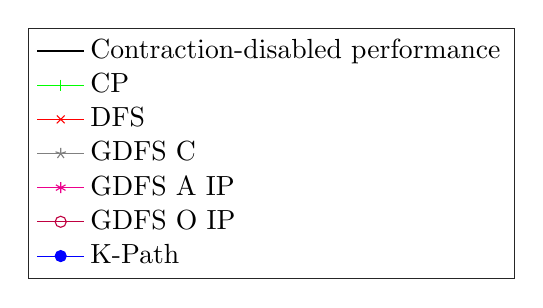
\begin{tikzpicture} 
    \begin{axis}[%
    hide axis,
    xmin=10,
    xmax=50,
    ymin=0,
    ymax=0.4,
    legend style={draw=white!15!black,legend cell align=left}
    ]
	\addlegendimage{black}
    \addlegendentry{Contraction-disabled performance}; 
     
    \addlegendimage{green, mark=+}
    \addlegendentry{CP};
    
    \addlegendimage{red, mark=x}
    \addlegendentry{DFS};
    
    \addlegendimage{gray, mark=star}
    \addlegendentry{GDFS C};
    
    \addlegendimage{magenta, mark=asterisk}
    \addlegendentry{GDFS A IP};
    
    \addlegendimage{purple, mark=o}
    \addlegendentry{GDFS O IP};
    
    \addlegendimage{blue, mark=*}
    \addlegendentry{K-Path};
    
    \end{axis}
\end{tikzpicture}

\end{subfigure}

\caption{Mean relative time consumption of contraction-enabled subgraph homeomorphism search compared to contraction-disabled for different path iteration methods. For data points below the reference line contraction saves time while for data points above it contraction costs extra time. ``refuse longer paths" is disabled and no pruning is used. We handled a maximum of 1000 test cases or 10 minutes per value of $|V_S|$ for each path iteration method.}	
\label{fig:contraction-performance}
\end{figure}




\begin{figure}
\begin{subfigure}{.5\linewidth}
\centering

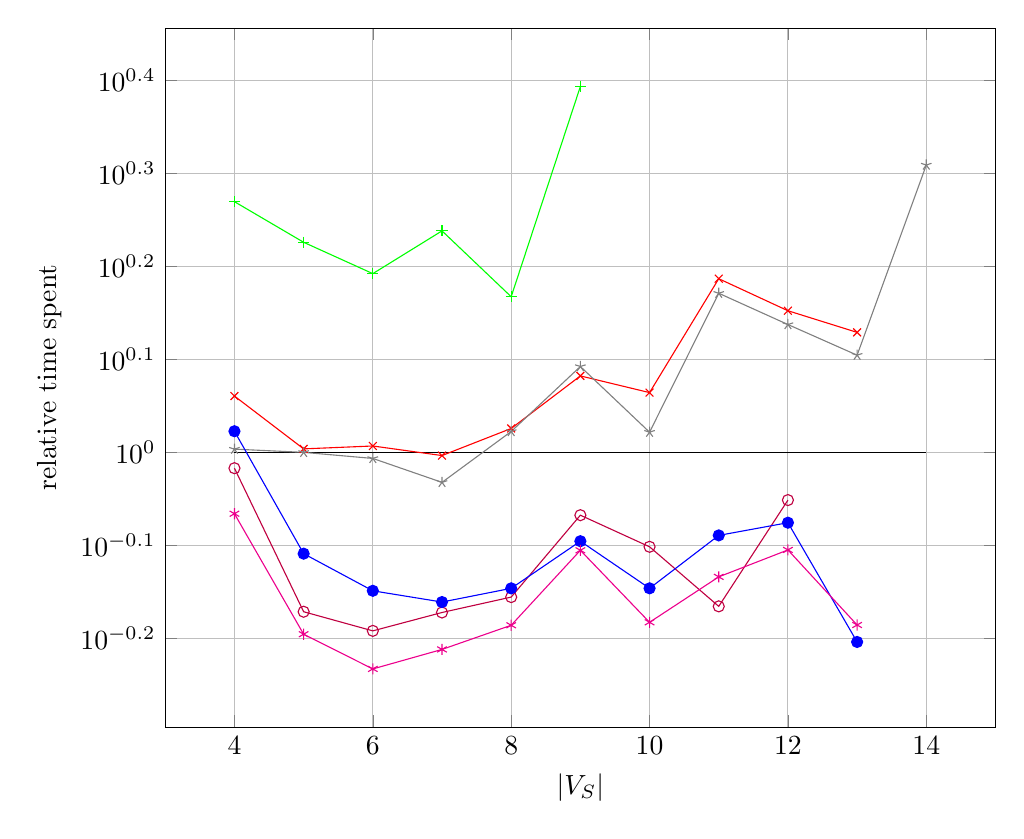
\begin{tikzpicture}
    \begin{axis}[
        xlabel=$|V_S|$,
        ylabel=relative time spent,
        ymode=log,
        legend style={at={(0.9,0.1)},anchor=south east},
        width=\textwidth,
		y tick label style={/pgf/number format/sci},
        ymajorgrids,
        xmajorgrids,		
    ]
\addplot [mark=none, black] plot coordinates {
        (4,1) (14,1)};

   

\addplot[
        mark=x,
        red,
    ] plot coordinates {
        (4,1.149235278417448)
        (5,1.0083079007951214)
        (6,1.015552114217333)
        (7,0.9917637188145205)
        (8,1.060601873501574)
        (9,1.2080204277209134)
        (10,1.1590683500674202)
        (11,1.5368985401765969)
        (12,1.4196166165898805)
        (13,1.345479282144217)
};
%    \addlegendentry{DFS}


\addplot[
        mark=o,
        purple,
    ] plot coordinates {
        (4,0.9612291827097055)
        (5,0.6736846557006542)
        (6,0.6425091767491988)
        (7,0.6723934364944264)
        (8,0.6986220309175226)
        (9,0.8556489486454084)
        (10,0.7913299276289911)
        (11,0.6827413496042884)
        (12,0.8882442635255605)
};
%    \addlegendentry{GDFS O IP}


\addplot[
        mark=star,
        gray,
    ] plot coordinates {
        (4,1.0076438451392467)
        (5,0.9996588783961261)
        (6,0.9847179505164285)
        (7,0.9280395733234135)
        (8,1.052698920988995)
        (9,1.2364165435036165)
        (10,1.0508458659524293)
        (11,1.482398673483428)
        (12,1.3719047068368444)
        (13,1.2716510858517898)
        (14,2.0364819148591398)
};
%    \addlegendentry{GDFS C}


\addplot[
        mark=*,
        blue,
    ] plot coordinates {
        (4,1.0533520014717994)
        (5,0.7778922096030297)
        (6,0.7095420859821555)
        (7,0.690031519800899)
        (8,0.7138989512612041)
        (9,0.8022495198052423)
        (10,0.7139100327511367)
        (11,0.8138526765920138)
        (12,0.839844649957909)
        (13,0.6251267562387761)
};
%    \addlegendentry{K-Path}


\addplot[
        mark=+,
        green,
    ] plot coordinates {
        (4,1.8598817420849323)
        (5,1.6819321086529642)
        (6,1.5562633425290353)
        (7,1.7300402065586273)
        (8,1.4697328084299048)
        (9,2.4737693466393464)
};
%    \addlegendentry{CP}


\addplot[
        mark=asterisk,
        magenta,
    ] plot coordinates {
        (4,0.8587470004926293)
        (5,0.637211123426433)
        (6,0.5846797577876022)
        (7,0.6136474407419334)
        (8,0.6515146194296546)
        (9,0.7843995636829644)
        (10,0.6563231931888491)
        (11,0.7344868290598967)
        (12,0.7852380262879831)
        (13,0.6519427807384649)
};
%    \addlegendentry{GDFS A IP}


   

    \end{axis}
    \end{tikzpicture}


\caption{Serial}
\end{subfigure}%
\begin{subfigure}{.5\linewidth}
\centering

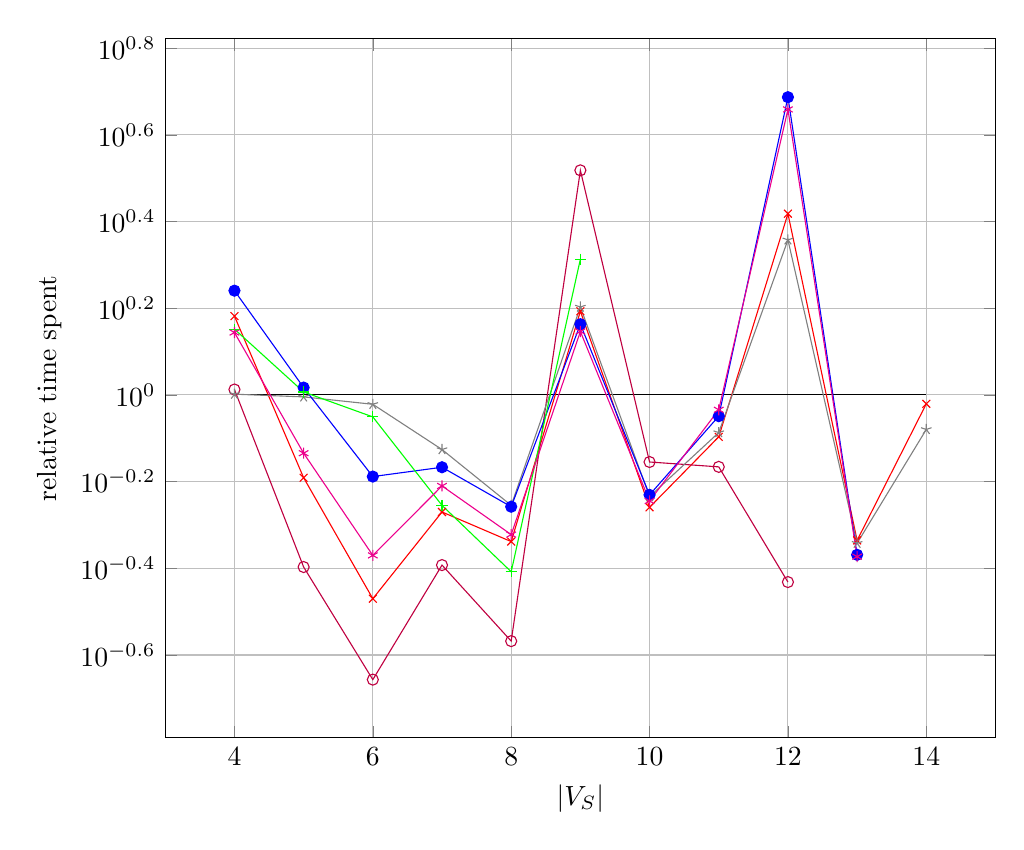
\begin{tikzpicture}
    \begin{axis}[
        xlabel=$|V_S|$,
        ylabel=relative time spent,
        ymode=log,
        legend style={at={(0.9,0.1)},anchor=south east},
        width=\textwidth,
		y tick label style={/pgf/number format/sci},
        ymajorgrids,
        xmajorgrids,		
    ]
\addplot [mark=none, black] plot coordinates {
        (4,1) (14, 1)};




\addplot[
        mark=x,
        red,
    ] plot coordinates {
        (4,1.5196735481803552)
        (5,0.6439969153711)
        (6,0.3386925334619767)
        (7,0.5368610674342231)
        (8,0.45873474922274815)
        (9,1.5594868514866573)
        (10,0.5503271443080898)
        (11,0.8002158520089797)
        (12,2.618829716025611)
        (13,0.461660681606467)
        (14,0.9536983450489754)
};
%    \addlegendentry{DFS}


\addplot[
        mark=o,
        purple,
    ] plot coordinates {
        (4,1.0289639751297441)
        (5,0.40073099730691264)
        (6,0.2203309298278896)
        (7,0.40490458510733796)
        (8,0.2703553467095787)
        (9,3.2968841136523857)
        (10,0.7001969451830652)
        (11,0.6822506009880664)
        (12,0.37004898049509893)
};
%    \addlegendentry{GDFS O IP}


\addplot[
        mark=star,
        gray,
    ] plot coordinates {
        (4,1.0037860591934256)
        (5,0.9894012765779054)
        (6,0.9512995639254895)
        (7,0.7481500768569231)
        (8,0.5560328419142169)
        (9,1.5950594125932698)
        (10,0.5825880979420317)
        (11,0.8186254429321587)
        (12,2.2787645869722217)
        (13,0.4547207271773557)
        (14,0.8323681075075677)
};
%    \addlegendentry{GDFS C}


\addplot[
        mark=*,
        blue,
    ] plot coordinates {
        (4,1.739824792303458)
        (5,1.0396016144545588)
        (6,0.6479907091747379)
        (7,0.6809036260493723)
        (8,0.5520901104899674)
        (9,1.4556125513833869)
        (10,0.5879764504015326)
        (11,0.8930337054115022)
        (12,4.862531350090637)
        (13,0.4275493552859416)
};
%    \addlegendentry{K-Path}


\addplot[
        mark=+,
        green,
    ] plot coordinates {
        (4,1.4181640975707355)
        (5,1.0155919393670438)
        (6,0.8896407770170547)
        (7,0.5560547295333215)
        (8,0.3908257237814686)
        (9,2.0567874784311706)
};
%    \addlegendentry{CP}


\addplot[
        mark=asterisk,
        magenta,
    ] plot coordinates {
        (4,1.3928057135978327)
        (5,0.7336372164409364)
        (6,0.4262986752445699)
        (7,0.6165329994701355)
        (8,0.47610065673013646)
        (9,1.4003560173584488)
        (10,0.5691849125616277)
        (11,0.9238715681263124)
        (12,4.55583983031228)
        (13,0.4234248244588815)
};
%    \addlegendentry{GDFS A IP}
  

	
    \end{axis}
    \end{tikzpicture}

\caption{Cached}
\end{subfigure}\\[1ex]
\begin{subfigure}{0.5\linewidth}
\centering

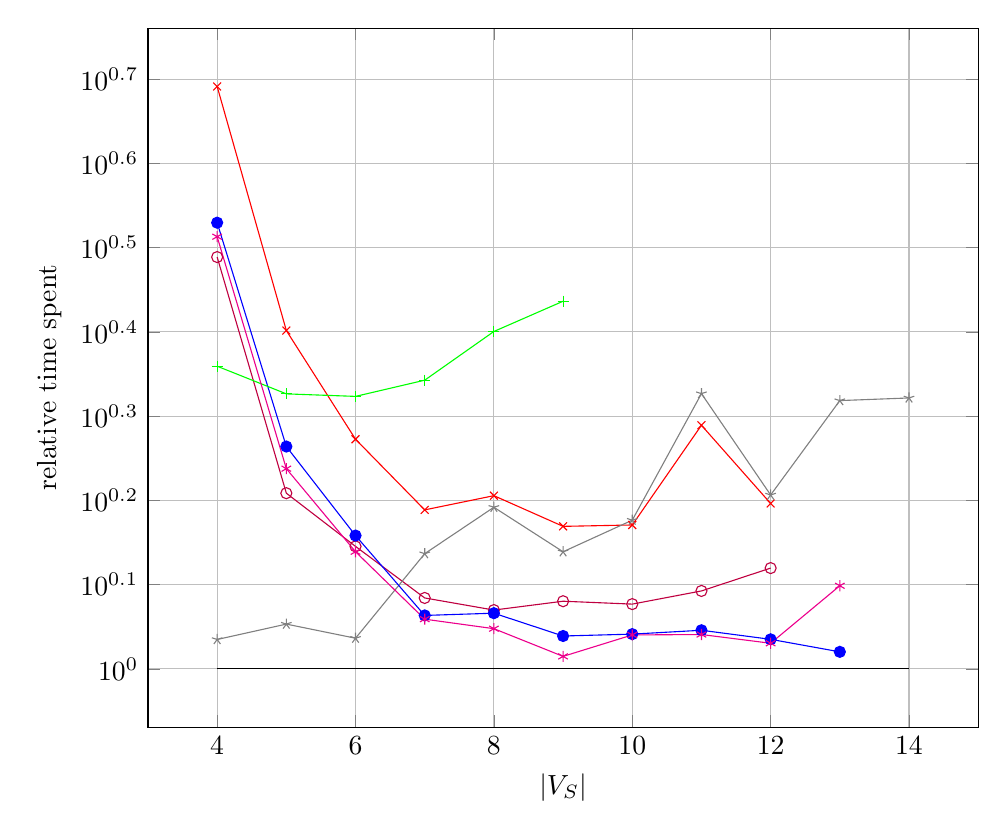
\begin{tikzpicture}
    \begin{axis}[
        xlabel=$|V_S|$,
        ylabel=relative time spent,
        ymode=log,
        legend style={at={(0.9,0.1)},anchor=south east},
        width=\textwidth,
		y tick label style={/pgf/number format/sci},
        ymajorgrids,
        xmajorgrids,		
    ]
\addplot [mark=none, black] plot coordinates {
        (4,1) (14, 1)};


	

\addplot[
        mark=x,
        red,
    ] plot coordinates {
        (4,4.912635821328207)
        (5,2.5213322807291894)
        (6,1.8735281366916912)
        (7,1.5444862545247475)
        (8,1.6056787150146559)
        (9,1.4765521555469698)
        (10,1.4820555556240134)
        (11,1.946734238439349)
        (12,1.5718556269712267)
};
%    \addlegendentry{DFS}


\addplot[
        mark=o,
        purple,
    ] plot coordinates {
        (4,3.0822240524751128)
        (5,1.6165571205344698)
        (6,1.3978485397981901)
        (7,1.2140415216311997)
        (8,1.1745946191206549)
        (9,1.2032865829671746)
        (10,1.1937969470403793)
        (11,1.2375642924085462)
        (12,1.3172897955473268)
};
%    \addlegendentry{GDFS O IP}


\addplot[
        mark=star,
        gray,
    ] plot coordinates {
        (4,1.0837979979749324)
        (5,1.1303336976253304)
        (6,1.087572597425233)
        (7,1.3702576979065668)
        (8,1.5556435786427398)
        (9,1.3774635843717524)
        (10,1.5016451292498205)
        (11,2.122041244880633)
        (12,1.6087569895860554)
        (13,2.0820432556276365)
        (14,2.09712979447583)
};
%    \addlegendentry{GDFS C}


\addplot[
        mark=*,
        blue,
    ] plot coordinates {
        (4,3.38561160720786)
        (5,1.8365969772716313)
        (6,1.4398010790115316)
        (7,1.1574587494667208)
        (8,1.1645623226507533)
        (9,1.0941954726393444)
        (10,1.099782306968)
        (11,1.1114580211799494)
        (12,1.0842992282419759)
        (13,1.0478118522343631)
};
%    \addlegendentry{K-Path}


\addplot[
        mark=+,
        green,
    ] plot coordinates {
        (4,2.287168110582633)
        (5,2.120634315355006)
        (6,2.1061165486427873)
        (7,2.2013837152903006)
        (8,2.514842573582901)
        (9,2.731646143463003)
};
%    \addlegendentry{CP}


\addplot[
        mark=asterisk,
        magenta,
    ] plot coordinates {
        (4,3.2585173952994615)
        (5,1.728583400469593)
        (6,1.3775627829587174)
        (7,1.1456803324069784)
        (8,1.1162737735571762)
        (9,1.0349155153974534)
        (10,1.0973729419863378)
        (11,1.098601313310929)
        (12,1.0726988929900587)
        (13,1.2552103868339886)
};
%    \addlegendentry{GDFS A IP}

	
	
    \end{axis}
    \end{tikzpicture}

\caption{Parallel}
\end{subfigure}
\begin{subfigure} {0.5\linewidth}
\centering

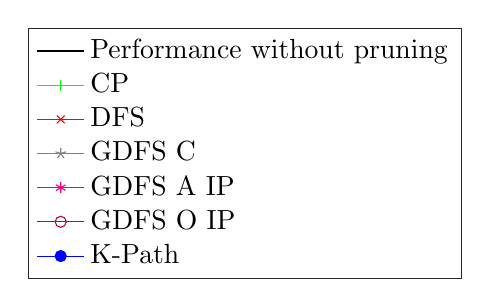
\begin{tikzpicture} 
    \begin{axis}[%
    hide axis,
    xmin=10,
    xmax=50,
    ymin=0,
    ymax=0.4,
    legend style={draw=white!15!black,legend cell align=left}
    ]
	\addlegendimage{black}
    \addlegendentry{Performance without pruning}; 
     
    \addlegendimage{green, mark=+}
    \addlegendentry{CP};
    
    \addlegendimage{red, mark=x}
    \addlegendentry{DFS};
    
    \addlegendimage{gray, mark=star}
    \addlegendentry{GDFS C};
    
    \addlegendimage{magenta, mark=asterisk}
    \addlegendentry{GDFS A IP};
    
    \addlegendimage{purple, mark=o}
    \addlegendentry{GDFS O IP};
    
    \addlegendimage{blue, mark=*}
    \addlegendentry{K-Path};
    
    \end{axis}
\end{tikzpicture}

\end{subfigure}

\caption{Performance of our algorithm with \textbf{ZeroDomain} pruning using \textbf{`Labels and neighbours'} filtering relative to the performance of the algorithm without pruning. $|V_T|=1\frac{1}{2}*|V_S|$, ``refuse longer paths" and contraction are disabled and we use the degree-based target graph vertex ordering. Data points above the black reference line denote that the pruning method introduces more delay, and data points below the reference line denote that the pruning method saves time. Note the logarithmic y-axis.}	
\label{fig:zerodomainlabelsneighbours}
\end{figure}



\begin{figure}
\begin{subfigure}{.5\linewidth}
\centering

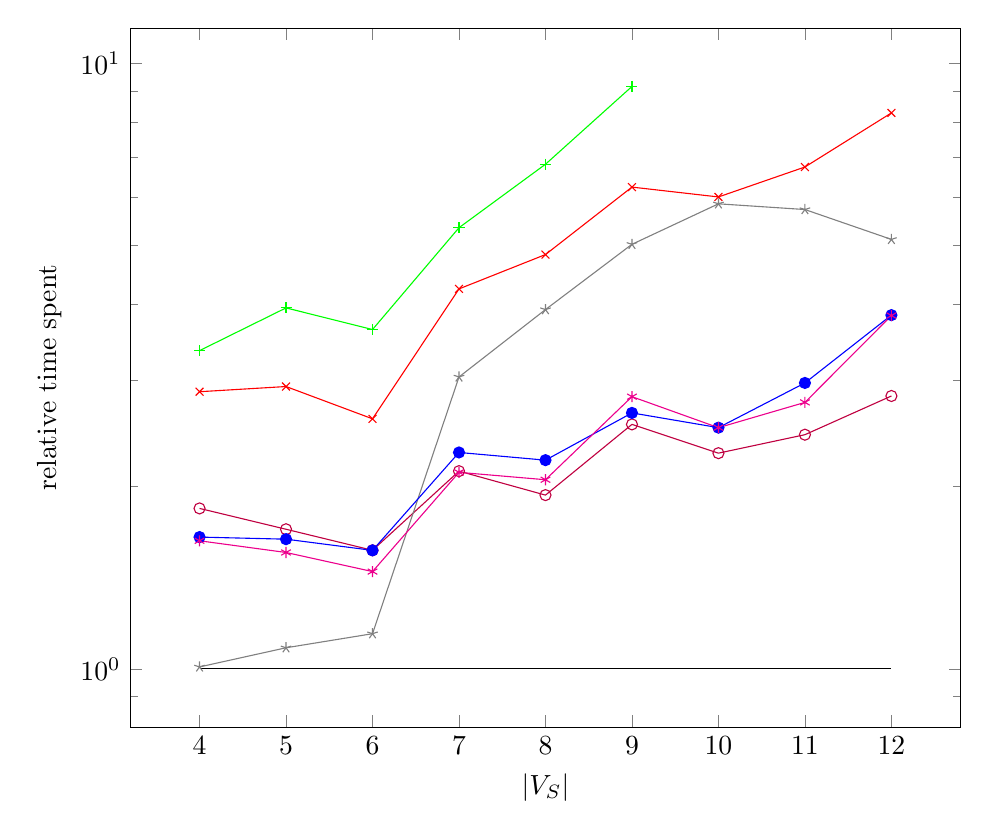
\begin{tikzpicture}
    \begin{axis}[
        xlabel=$|V_S|$,
        ylabel=relative time spent,
        ymode=log,
        legend style={at={(0.9,0.1)},anchor=south east},
        width=\textwidth,
		y tick label style={/pgf/number format/sci},
    ]
\addplot [mark=none, black] plot coordinates {
        (4,1) (12, 1)};

    

\addplot[
        mark=x,
        red,
    ] plot coordinates {
        (4,2.8681701535417203)
        (5,2.9254018783511473)
        (6,2.5872798141640203)
        (7,4.239345235159544)
        (8,4.830571894920121)
        (9,6.242761798378523)
        (10,6.013058042923716)
        (11,6.738597774875578)
        (12,8.275599621231075)
};
%    \addlegendentry{DFS}


\addplot[
        mark=o,
        purple,
    ] plot coordinates {
        (4,1.8408080356188123)
        (5,1.7005582324670065)
        (6,1.56989493549955)
        (7,2.1207796500463942)
        (8,1.9363735218126932)
        (9,2.533248243975908)
        (10,2.2707880019469786)
        (11,2.4359352917004715)
        (12,2.821912275157622)
};
%    \addlegendentry{GDFS O IP}


\addplot[
        mark=star,
        gray,
    ] plot coordinates {
        (4,1.0076654131165232)
        (5,1.0837612058063686)
        (6,1.1432927339149115)
        (7,3.033634347762899)
        (8,3.919309944661518)
        (9,5.022580039736159)
        (10,5.858260568094502)
        (11,5.732626441781628)
        (12,5.117036438110539)
};
%    \addlegendentry{GDFS C}


\addplot[
        mark=*,
        blue,
    ] plot coordinates {
        (4,1.6507129093587034)
        (5,1.6376785905633322)
        (6,1.5694034681484315)
        (7,2.2768378662823556)
        (8,2.2111751094243637)
        (9,2.6460554936280003)
        (10,2.5019612966868143)
        (11,2.9653929534687484)
        (12,3.8377325981845987)
};
%    \addlegendentry{K-Path}


\addplot[
        mark=+,
        green,
    ] plot coordinates {
        (4,3.3530620508044278)
        (5,3.945082943073584)
        (6,3.633181121338477)
        (7,5.349792316707754)
        (8,6.809444287637352)
        (9,9.151106021332374)
};
%    \addlegendentry{CP}


\addplot[
        mark=asterisk,
        magenta,
    ] plot coordinates {
        (4,1.6276085621719778)
        (5,1.5567783428027056)
        (6,1.447868814386046)
        (7,2.111238924804706)
        (8,2.052589583126582)
        (9,2.8147150464658517)
        (10,2.5017899929941634)
        (11,2.7540625611814193)
        (12,3.831399427105856)
};
%    \addlegendentry{GDFS A IP}

   

    \end{axis}
    \end{tikzpicture}


\caption{serial}

\end{subfigure}%
\begin{subfigure}{.5\linewidth}
\centering

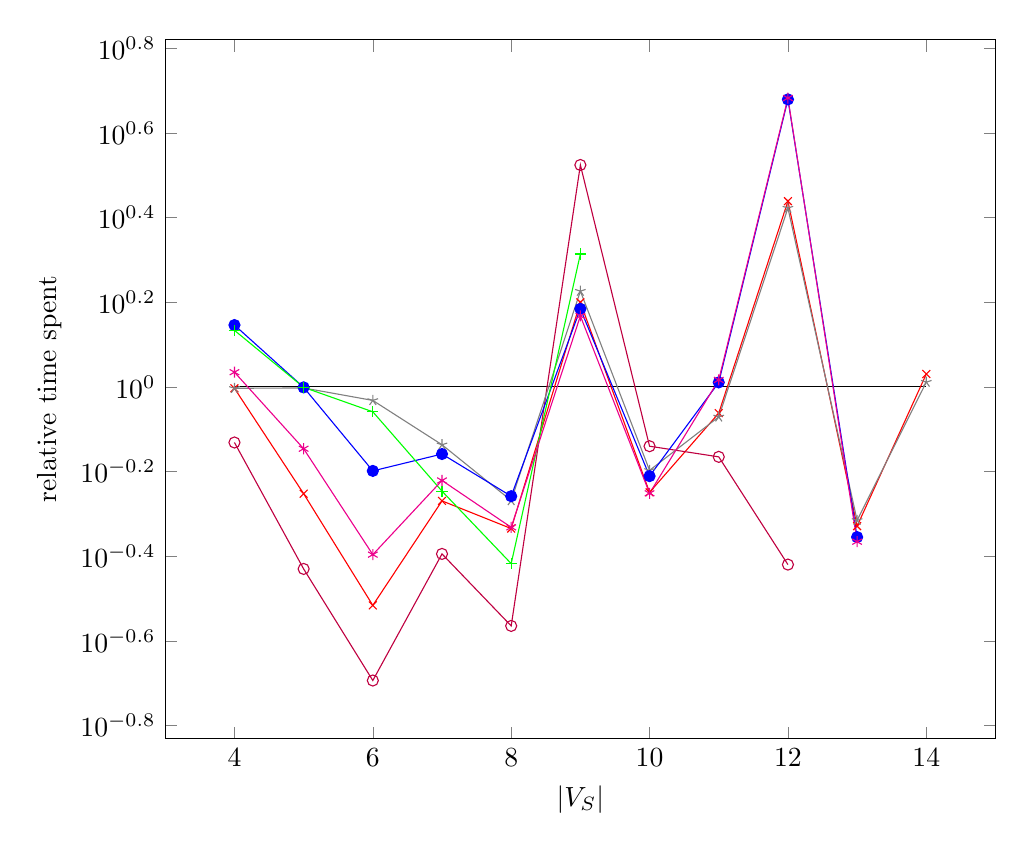
\begin{tikzpicture}
    \begin{axis}[
        xlabel=$|V_S|$,
        ylabel=relative time spent,
        ymode=log,
        legend style={at={(0.9,0.1)},anchor=south east},
        width=\textwidth,
		y tick label style={/pgf/number format/sci},
    ]
\addplot [mark=none, black] plot coordinates {
        (4,1) (14, 1)};


	

\addplot[
        mark=x,
        red,
    ] plot coordinates {
        (4,0.9923899104921649)
        (5,0.5595066683253078)
        (6,0.3048945865180337)
        (7,0.5381004704636452)
        (8,0.4628899334014771)
        (9,1.5833880688615796)
        (10,0.563696852962109)
        (11,0.8669963898068426)
        (12,2.745349524198522)
        (13,0.4690924414042419)
        (14,1.0728242665153411)
};
%    \addlegendentry{DFS}


\addplot[
        mark=o,
        purple,
    ] plot coordinates {
        (4,0.739244200124882)
        (5,0.3717240182715724)
        (6,0.20260979424571846)
        (7,0.40328082248328134)
        (8,0.2726428806815875)
        (9,3.342614987755728)
        (10,0.7244476709108397)
        (11,0.6836929828863543)
        (12,0.3805696273086222)
};
%    \addlegendentry{GDFS O IP}


\addplot[
        mark=star,
        gray,
    ] plot coordinates {
        (4,0.9924896603950555)
        (5,0.994360434712658)
        (6,0.9291538705872268)
        (7,0.730196682594658)
        (8,0.5390873818404287)
        (9,1.6832008614785352)
        (10,0.6352356062289578)
        (11,0.8496501176486361)
        (12,2.6445551844487807)
        (13,0.4840033554409139)
        (14,1.026259804661441)
};
%    \addlegendentry{GDFS C}


\addplot[
        mark=*,
        blue,
    ] plot coordinates {
        (4,1.3997982449312394)
        (5,0.997525391259792)
        (6,0.6333756640426693)
        (7,0.6943303320196079)
        (8,0.5519684346380963)
        (9,1.5286729452268917)
        (10,0.6156583962202479)
        (11,1.024740262929912)
        (12,4.774734990588401)
        (13,0.4419374709287728)
};
%    \addlegendentry{K-Path}


\addplot[
        mark=+,
        green,
    ] plot coordinates {
        (4,1.3603876642406472)
        (5,0.9977315311707801)
        (6,0.8734385188908586)
        (7,0.5673919611448295)
        (8,0.3826349700684204)
        (9,2.0597652911938544)
};
%    \addlegendentry{CP}


\addplot[
        mark=asterisk,
        magenta,
    ] plot coordinates {
        (4,1.0832036968767507)
        (5,0.714551103294575)
        (6,0.4017364306204272)
        (7,0.6012055707935953)
        (8,0.4660022392983759)
        (9,1.4709429657453295)
        (10,0.5607915060867077)
        (11,1.0386348465457822)
        (12,4.8097603627365055)
        (13,0.43097398458603053)
};
%    \addlegendentry{GDFS A IP}

	
    \end{axis}
    \end{tikzpicture}

\caption{cached}

\end{subfigure}\\[1ex]
\begin{subfigure}{0.5\linewidth}
\centering

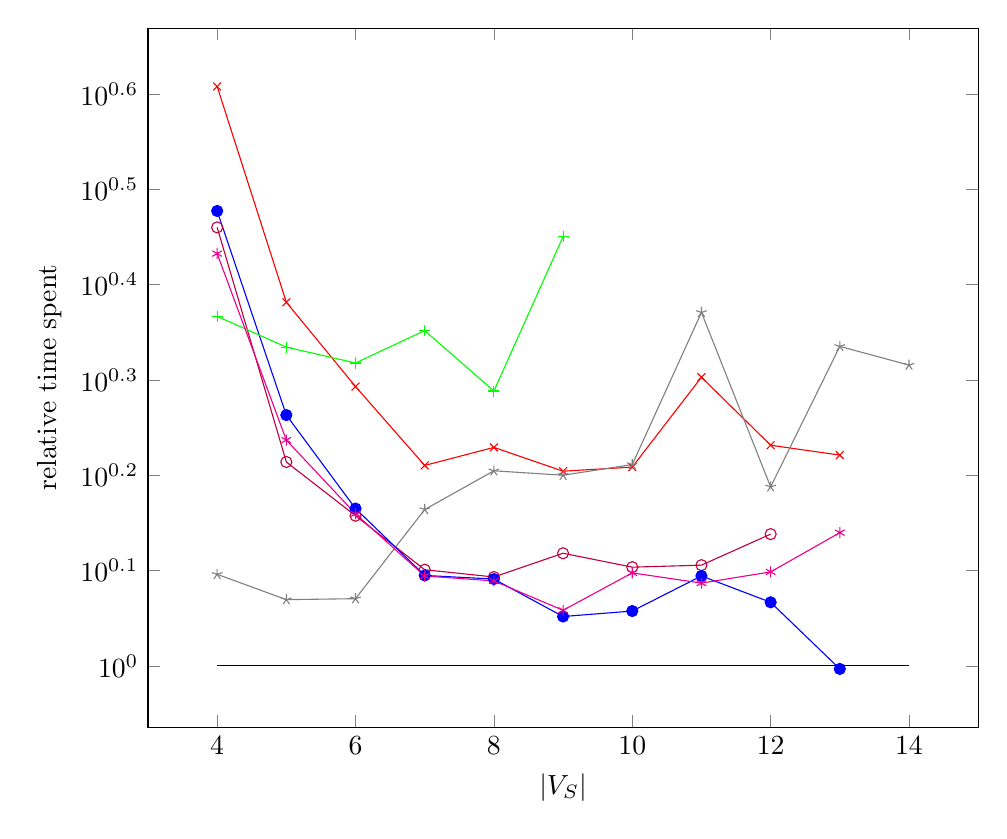
\begin{tikzpicture}
    \begin{axis}[
        xlabel=$|V_S|$,
        ylabel=relative time spent,
        ymode=log,
        legend style={at={(0.9,0.1)},anchor=south east},
        width=\textwidth,
		y tick label style={/pgf/number format/sci},
    ]
\addplot [mark=none, black] plot coordinates {
        (4,1) (14, 1)};



\addplot[
        mark=x,
        red,
    ] plot coordinates {
        (4,4.055665332528571)
        (5,2.4079068291217)
        (6,1.9643320384841314)
        (7,1.6232718485965263)
        (8,1.6955903014633646)
        (9,1.6008062270872792)
        (10,1.6167961960677952)
        (11,2.008933357310069)
        (12,1.704410962543426)
        (13,1.6643657926641058)
};
%    \addlegendentry{DFS}


\addplot[
        mark=o,
        purple,
    ] plot coordinates {
        (4,2.8851878090262195)
        (5,1.636942509871993)
        (6,1.4374997042728976)
        (7,1.2616655204621405)
        (8,1.2396952026488233)
        (9,1.3129460412244731)
        (10,1.269489134852407)
        (11,1.2756554118663406)
        (12,1.3750472085101815)
};
%    \addlegendentry{GDFS O IP}


\addplot[
        mark=star,
        gray,
    ] plot coordinates {
        (4,1.2478328793750295)
        (5,1.1736817816635776)
        (6,1.1764101574372858)
        (7,1.4592075490444798)
        (8,1.6024676243054734)
        (9,1.5853180312626138)
        (10,1.6267475153944102)
        (11,2.3492273224066422)
        (12,1.541367629203128)
        (13,2.1643253277100984)
        (14,2.068648556937112)
};
%    \addlegendentry{GDFS C}


\addplot[
        mark=*,
        blue,
    ] plot coordinates {
        (4,3.002052014953125)
        (5,1.8333632864658882)
        (6,1.4625868876088735)
        (7,1.244428892395309)
        (8,1.2334917943953325)
        (9,1.1267969028185083)
        (10,1.1417960691621196)
        (11,1.242845045792521)
        (12,1.1662050312002787)
        (13,0.9927656897482176)
};
%    \addlegendentry{K-Path}


\addplot[
        mark=+,
        green,
    ] plot coordinates {
        (4,2.327075300876756)
        (5,2.160407689989366)
        (6,2.0792574180238432)
        (7,2.248434541176637)
        (8,1.943200046149185)
        (9,2.82171519727411)
};
%    \addlegendentry{CP}


\addplot[
        mark=asterisk,
        magenta,
    ] plot coordinates {
        (4,2.7083657638964724)
        (5,1.7258042096013082)
        (6,1.4441565938470444)
        (7,1.2427090481371263)
        (8,1.2279821585739619)
        (9,1.1438554945469597)
        (10,1.252073988123748)
        (11,1.2215012813271526)
        (12,1.2550832966834882)
        (13,1.3798442157135253)
};
%    \addlegendentry{GDFS A IP}

	
    \end{axis}
    \end{tikzpicture}

\caption{parallel}

\end{subfigure}
\begin{subfigure} {0.5\linewidth}
\centering

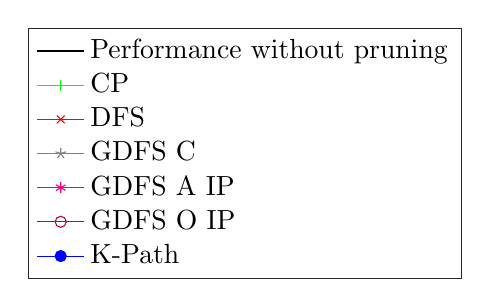
\begin{tikzpicture} 
    \begin{axis}[%
    hide axis,
    xmin=10,
    xmax=50,
    ymin=0,
    ymax=0.4,
    legend style={draw=white!15!black,legend cell align=left}
    ]
	\addlegendimage{black}
    \addlegendentry{Performance without pruning}; 
     
    \addlegendimage{green, mark=+}
    \addlegendentry{CP};
    
    \addlegendimage{red, mark=x}
    \addlegendentry{DFS};
    
    \addlegendimage{gray, mark=star}
    \addlegendentry{GDFS C};
    
    \addlegendimage{magenta, mark=asterisk}
    \addlegendentry{GDFS A IP};
    
    \addlegendimage{purple, mark=o}
    \addlegendentry{GDFS O IP};
    
    \addlegendimage{blue, mark=*}
    \addlegendentry{K-Path};
    
    \end{axis}
\end{tikzpicture}

\end{subfigure}

\caption{Performance of our algorithm with \textbf{ZeroDomain} pruning using \textbf{`Free neighbours'} filtering relative to the performance of the algorithm without pruning. We avoid unnecessarily long paths, do not perform contraction and use the degree-based target graph vertex ordering. Data points above the black reference line denote that the pruning method introduces more delay, and data points below the reference line denote that the pruning method saves time. Note the logarithmic y-axis.}	
\label{fig:zerodomainunmatched}
\end{figure}


\begin{figure}
\begin{subfigure}{.5\linewidth}
\centering

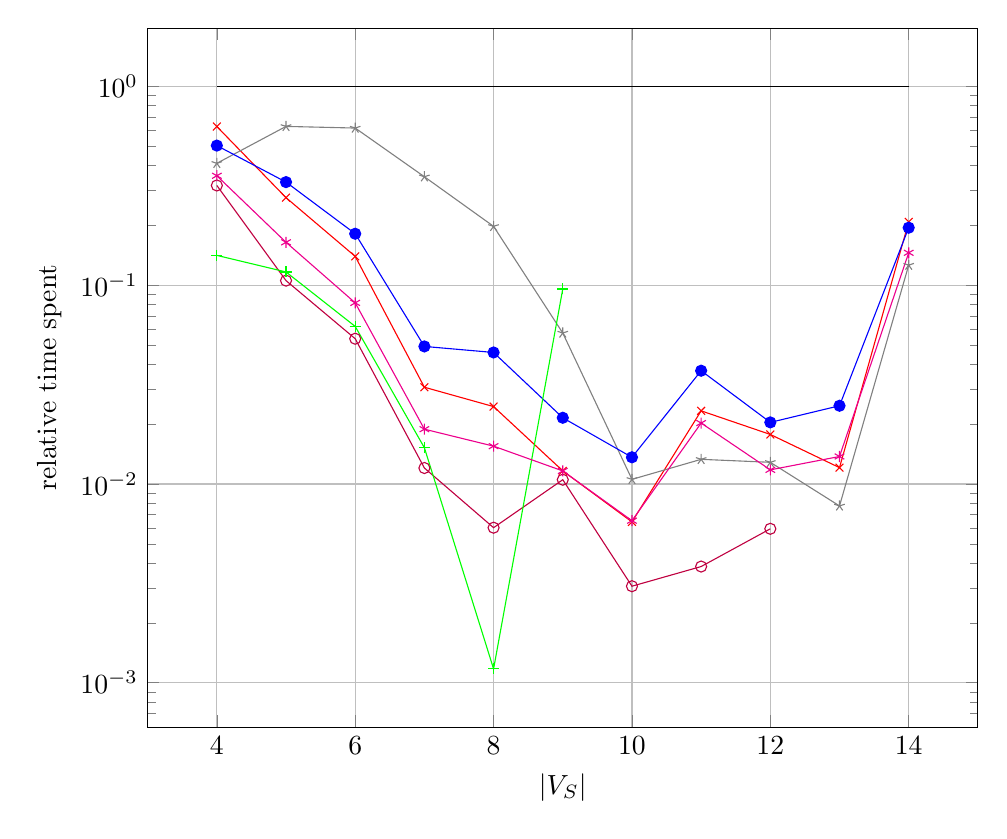
\begin{tikzpicture}
        \begin{axis}[
        xlabel=$|V_S|$,
        ylabel=relative time spent,
        ymode=log,
        legend style={at={(0.9,0.1)},anchor=south east},
        width=\textwidth,
		y tick label style={/pgf/number format/sci},
        ymajorgrids,
        xmajorgrids,		
    ]
\addplot [mark=none, black] plot coordinates {
        (4,1) (14, 1)};



\addplot[
        mark=x,
        red,
    ] plot coordinates {
        (4,0.6287543277612293)
        (5,0.2757977099154991)
        (6,0.1396777930920231)
        (7,0.030673609879429353)
        (8,0.02451224889378789)
        (9,0.011639988009323088)
        (10,0.006444926208946211)
        (11,0.023332165971646113)
        (12,0.017747881691377088)
        (13,0.012081584812504542)
        (14,0.20827170338997036)
};
%    \addlegendentry{DFS}


\addplot[
        mark=o,
        purple,
    ] plot coordinates {
        (4,0.31762184661225146)
        (5,0.10548661997054809)
        (6,0.05380597268481946)
        (7,0.012031104647835078)
        (8,0.006026685633755746)
        (9,0.010506576117209399)
        (10,0.003059622842895182)
        (11,0.0038425576274282447)
        (12,0.005950005569221872)
};
%    \addlegendentry{GDFS O IP}


\addplot[
        mark=star,
        gray,
    ] plot coordinates {
        (4,0.4106300255336265)
        (5,0.6297150335729914)
        (6,0.6177849466375939)
        (7,0.3514224232413242)
        (8,0.1978056188420405)
        (9,0.05747899493182684)
        (10,0.01054844071183747)
        (11,0.013304423784248232)
        (12,0.01285276131493418)
        (13,0.007754862312966293)
        (14,0.12620402164239297)
};
%    \addlegendentry{GDFS C}


\addplot[
        mark=*,
        blue,
    ] plot coordinates {
        (4,0.5042771733798161)
        (5,0.33026481004490515)
        (6,0.1815749814615767)
        (7,0.04920860049799136)
        (8,0.04588175630434421)
        (9,0.02153377003082302)
        (10,0.013622516633218007)
        (11,0.037145391651794424)
        (12,0.02041196505471854)
        (13,0.024748365975288622)
        (14,0.19477391590054371)
};
%    \addlegendentry{K-Path}


\addplot[
        mark=+,
        green,
    ] plot coordinates {
        (4,0.14129388384266495)
        (5,0.11661297643581336)
        (6,0.062037664925466474)
        (7,0.015214384516616386)
        (8,0.001173447995948207)
        (9,0.09577023175742294)
};
%    \addlegendentry{CP}


\addplot[
        mark=asterisk,
        magenta,
    ] plot coordinates {
        (4,0.35547913440959544)
        (5,0.16441492185647066)
        (6,0.081522356518962)
        (7,0.01887115321256927)
        (8,0.015496754850373495)
        (9,0.01163137758041799)
        (10,0.0065360121014294)
        (11,0.02025243713993974)
        (12,0.011777226097555493)
        (13,0.013750262714309236)
        (14,0.1456191628467376)
};
%    \addlegendentry{GDFS A IP}


   

    \end{axis}
    \end{tikzpicture}


\caption{serial}

\end{subfigure}%
\begin{subfigure}{.5\linewidth}
\centering

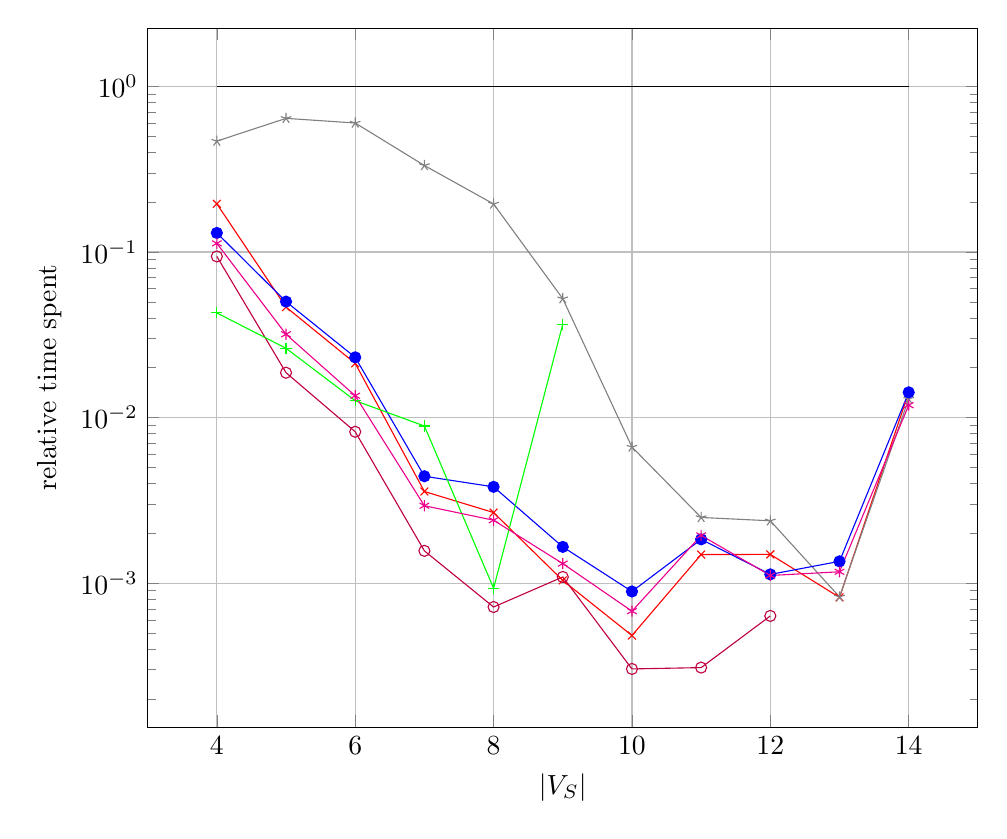
\begin{tikzpicture}
       \begin{axis}[
        xlabel=$|V_S|$,
        ylabel=relative time spent,
        ymode=log,
        legend style={at={(0.9,0.1)},anchor=south east},
        width=\textwidth,
		y tick label style={/pgf/number format/sci},
        ymajorgrids,
        xmajorgrids,		
    ]
\addplot [mark=none, black] plot coordinates {
        (4,1) (14, 1)};



\addplot[
        mark=x,
        red,
    ] plot coordinates {
        (4,0.19553736011435197)
        (5,0.04651353813878456)
        (6,0.021254007864093483)
        (7,0.003578003137043706)
        (8,0.002669239461236206)
        (9,0.001038638013086457)
        (10,4.827831034437402E-4)
        (11,0.0014882311568104045)
        (12,0.0014918153191871841)
        (13,8.201888846909311E-4)
        (14,0.014177555092282024)
};
%    \addlegendentry{DFS}


\addplot[
        mark=o,
        purple,
    ] plot coordinates {
        (4,0.0940851187730316)
        (5,0.018669179394963042)
        (6,0.008210777047784168)
        (7,0.00156671351986859)
        (8,7.175769161658074E-4)
        (9,0.0010901108792181757)
        (10,3.032823855272371E-4)
        (11,3.089718288207255E-4)
        (12,6.339461008270098E-4)
};
%    \addlegendentry{GDFS O IP}


\addplot[
        mark=star,
        gray,
    ] plot coordinates {
        (4,0.46776174984809504)
        (5,0.6418994975058616)
        (6,0.6016705469416976)
        (7,0.33331288068306)
        (8,0.19516359829459384)
        (9,0.052258028899510256)
        (10,0.00663966390973203)
        (11,0.002493325643069144)
        (12,0.002380331383759815)
        (13,8.261279519951037E-4)
        (14,0.012952744336981126)
};
%    \addlegendentry{GDFS C}


\addplot[
        mark=*,
        blue,
    ] plot coordinates {
        (4,0.13042500432875637)
        (5,0.050180114187121205)
        (6,0.023114568588865403)
        (7,0.004422648284462927)
        (8,0.0038176084846363034)
        (9,0.0016559892479824923)
        (10,8.905816418131041E-4)
        (11,0.0018391391340257801)
        (12,0.0011295780527541543)
        (13,0.0013542664491973389)
        (14,0.01420206790590417)
};
%    \addlegendentry{K-Path}


\addplot[
        mark=+,
        green,
    ] plot coordinates {
        (4,0.0428754303586345)
        (5,0.026223845245723965)
        (6,0.012652891562625723)
        (7,0.008896499518256218)
        (8,9.31591774671725E-4)
        (9,0.03666836072401081)
};
%    \addlegendentry{CP}


\addplot[
        mark=asterisk,
        magenta,
    ] plot coordinates {
        (4,0.11278665322864612)
        (5,0.03186942103424617)
        (6,0.013551849864991583)
        (7,0.0029347571062988687)
        (8,0.0023993757390741166)
        (9,0.001312317141160979)
        (10,6.774056453796584E-4)
        (11,0.0019421604989434682)
        (12,0.0011128003583009694)
        (13,0.0011711624655019737)
        (14,0.011878755635911897)
};
%    \addlegendentry{GDFS A IP}

	
	
    \end{axis}
    \end{tikzpicture}

\caption{cached}

\end{subfigure}\\[1ex]
\begin{subfigure}{0.5\linewidth}
\centering

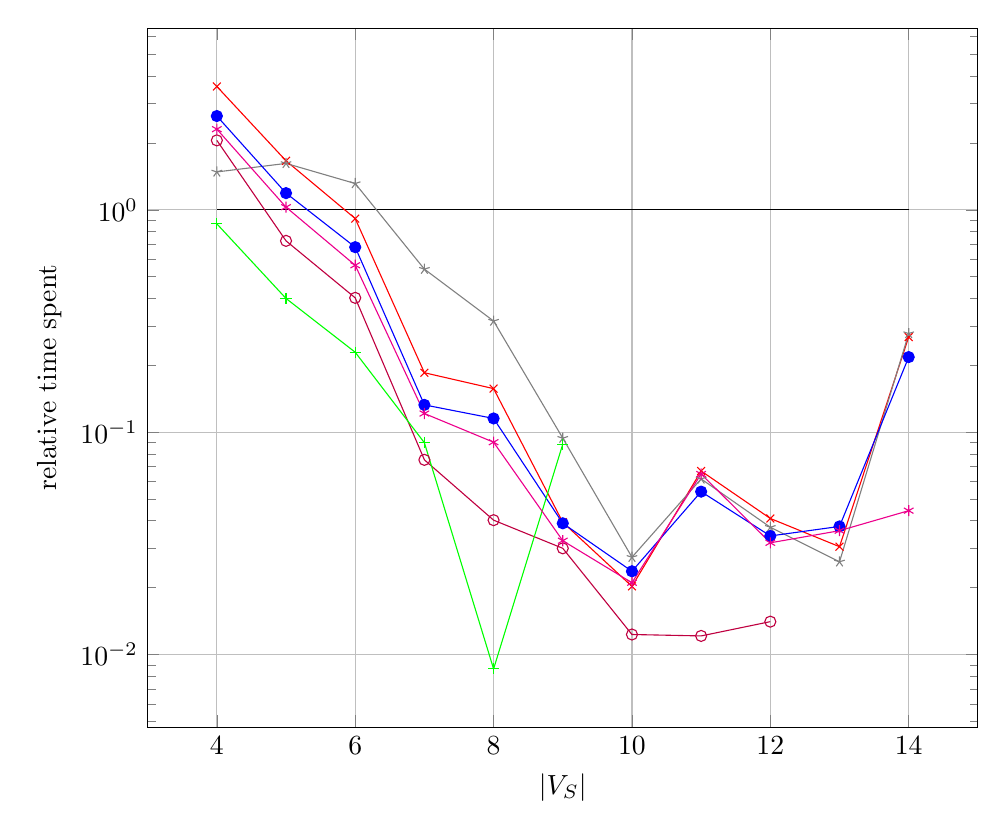
\begin{tikzpicture}
    \begin{axis}[
        xlabel=$|V_S|$,
        ylabel=relative time spent,
        ymode=log,
        legend style={at={(0.9,0.1)},anchor=south east},
        width=\textwidth,
		y tick label style={/pgf/number format/sci},
        ymajorgrids,
        xmajorgrids,		
    ]
\addplot [mark=none, black] plot coordinates {
        (4,1) (14, 1)};



\addplot[
        mark=x,
        red,
    ] plot coordinates {
        (4,3.5863917566717767)
        (5,1.6614170135257829)
        (6,0.913341561725058)
        (7,0.18513401953197028)
        (8,0.15706371851369083)
        (9,0.039380360092514)
        (10,0.020272354245869484)
        (11,0.06693875268275729)
        (12,0.04094655208604481)
        (13,0.03057385975605409)
        (14,0.26792292492149405)
};
%    \addlegendentry{DFS}


\addplot[
        mark=o,
        purple,
    ] plot coordinates {
        (4,2.052763630992859)
        (5,0.7252220094219901)
        (6,0.4019908919869054)
        (7,0.0751392967924247)
        (8,0.0402321588998491)
        (9,0.030063816263190213)
        (10,0.012316567212513396)
        (11,0.012136049821184658)
        (12,0.01407028044173897)
};
%    \addlegendentry{GDFS O IP}


\addplot[
        mark=star,
        gray,
    ] plot coordinates {
        (4,1.4803263312981985)
        (5,1.617088480231661)
        (6,1.312985590310922)
        (7,0.541000232064156)
        (8,0.31621413493384876)
        (9,0.09404453831749748)
        (10,0.027408496020476347)
        (11,0.061673144974397576)
        (12,0.03739780619521971)
        (13,0.02614141264184211)
        (14,0.2777072903785752)
};
%    \addlegendentry{GDFS C}


\addplot[
        mark=*,
        blue,
    ] plot coordinates {
        (4,2.640444380229205)
        (5,1.1886881061231498)
        (6,0.6793824205820389)
        (7,0.13271318550783862)
        (8,0.11533183769943123)
        (9,0.038955674057646106)
        (10,0.023698433402264296)
        (11,0.0540615523126724)
        (12,0.034171466937311545)
        (13,0.03771279726019261)
        (14,0.21769075053049192)
};
%    \addlegendentry{K-Path}


\addplot[
        mark=+,
        green,
    ] plot coordinates {
        (4,0.8650360306803884)
        (5,0.39951182944872243)
        (6,0.2288811300337159)
        (7,0.0896782754536235)
        (8,0.008624199068128502)
        (9,0.08847130248188806)
};
%    \addlegendentry{CP}


\addplot[
        mark=asterisk,
        magenta,
    ] plot coordinates {
        (4,2.3056130434020963)
        (5,1.0279513694895468)
        (6,0.5632528558219363)
        (7,0.12138481892093078)
        (8,0.09017283243188468)
        (9,0.03252156535486139)
        (10,0.02104885765787201)
        (11,0.06488806314689854)
        (12,0.031829464045399214)
        (13,0.03607848508196143)
        (14,0.04438987254212279)
};
%    \addlegendentry{GDFS A IP}

	
    \end{axis}
    \end{tikzpicture}

\caption{parallel}

\end{subfigure}
\begin{subfigure} {0.5\linewidth}
\centering

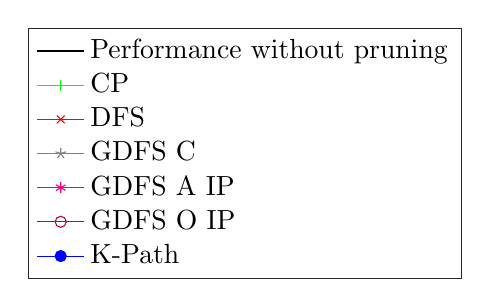
\begin{tikzpicture} 
    \begin{axis}[%
    hide axis,
    xmin=10,
    xmax=50,
    ymin=0,
    ymax=0.4,
    legend style={draw=white!15!black,legend cell align=left}
    ]
	\addlegendimage{black}
    \addlegendentry{Performance without pruning}; 
     
    \addlegendimage{green, mark=+}
    \addlegendentry{CP};
    
    \addlegendimage{red, mark=x}
    \addlegendentry{DFS};
    
    \addlegendimage{gray, mark=star}
    \addlegendentry{GDFS C};
    
    \addlegendimage{magenta, mark=asterisk}
    \addlegendentry{GDFS A IP};
    
    \addlegendimage{purple, mark=o}
    \addlegendentry{GDFS O IP};
    
    \addlegendimage{blue, mark=*}
    \addlegendentry{K-Path};
    
    \end{axis}
\end{tikzpicture}

\end{subfigure}

\caption{Performance of our algorithm with \textbf{ZeroDomain} pruning using \textbf{`M-filtering'} filtering relative to the performance of the algorithm without pruning. $|V_T|=1\frac{1}{2}*|V_S|$, ``refuse longer paths" and contraction are disabled and we use the degree-based target graph vertex ordering. Data points above the black reference line denote that the pruning method introduces more delay, and data points below the reference line denote that the pruning method saves time. Note the logarithmic y-axis.}	
\label{fig:zerodomainmfiltering}
\end{figure}


\begin{figure}
\begin{subfigure}{.5\linewidth}
\centering

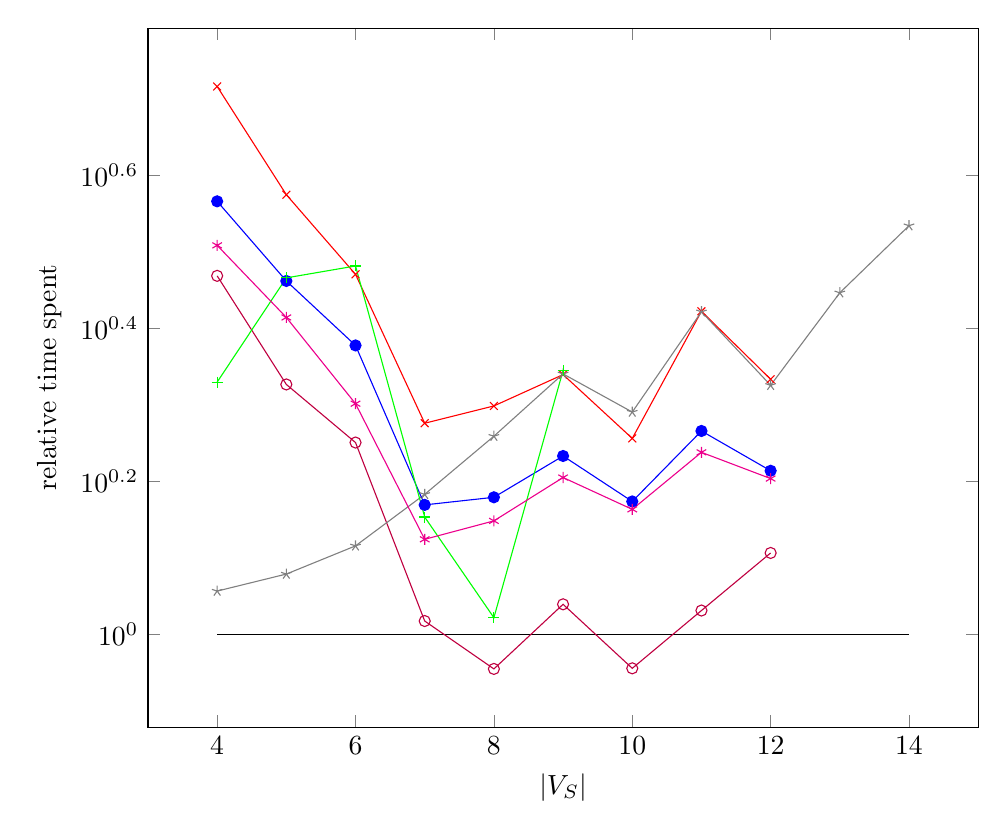
\begin{tikzpicture}
        \begin{axis}[
        xlabel=$|V_S|$,
        ylabel=relative time spent,
        ymode=log,
        legend style={at={(0.9,0.1)},anchor=south east},
        width=\textwidth,
		y tick label style={/pgf/number format/sci},
    ]
\addplot [mark=none, black] plot coordinates {
        (4,1) (14, 1)};

    
   

\addplot[
        mark=x,
        red,
    ] plot coordinates {
        (4,5.202946551261944)
        (5,3.756162046192574)
        (6,2.9549254023879072)
        (7,1.8872742557474473)
        (8,1.9880582223277101)
        (9,2.1847812854733193)
        (10,1.8028559351037163)
        (11,2.6436531391416507)
        (12,2.1539273359082483)
};
%    \addlegendentry{DFS}


\addplot[
        mark=o,
        purple,
    ] plot coordinates {
        (4,2.9414858115997387)
        (5,2.120863031356877)
        (6,1.7804930224229873)
        (7,1.0400701807728874)
        (8,0.9003554054490217)
        (9,1.0937936596519373)
        (10,0.9019831415298204)
        (11,1.0734764108654673)
        (12,1.2767276824510232)
};
%    \addlegendentry{GDFS O IP}


\addplot[
        mark=star,
        gray,
    ] plot coordinates {
        (4,1.1382355278673217)
        (5,1.198063456290179)
        (6,1.3042425098741526)
        (7,1.5233183009320665)
        (8,1.8148828000886499)
        (9,2.189451318312936)
        (10,1.9518249758925157)
        (11,2.639768817120566)
        (12,2.1154918845964863)
        (13,2.7952098947822313)
        (14,3.4210781907374623)
};
%    \addlegendentry{GDFS C}


\addplot[
        mark=*,
        blue,
    ] plot coordinates {
        (4,3.6819210072894446)
        (5,2.896400619358773)
        (6,2.3852188316658136)
        (7,1.4756755823523737)
        (8,1.5098085945063882)
        (9,1.7097753943529064)
        (10,1.490937989140139)
        (11,1.8438583447137513)
        (12,1.635315159939935)
};
%    \addlegendentry{K-Path}


\addplot[
        mark=+,
        green,
    ] plot coordinates {
        (4,2.1359021980392736)
        (5,2.923428609692478)
        (6,3.0304568963312812)
        (7,1.4225695726266137)
        (8,1.0506565420981449)
        (9,2.212314905046649)
};
%    \addlegendentry{CP}


\addplot[
        mark=asterisk,
        magenta,
    ] plot coordinates {
        (4,3.2242822734185275)
        (5,2.5950345747500103)
        (6,2.0014242504647624)
        (7,1.3303134982815363)
        (8,1.4062726411755775)
        (9,1.6024494454371436)
        (10,1.4559250035524376)
        (11,1.7288683972843149)
        (12,1.5973164420401704)
};
%    \addlegendentry{GDFS A IP}


    \end{axis}
    \end{tikzpicture}


\caption{serial}

\end{subfigure}%
\begin{subfigure}{.5\linewidth}
\centering

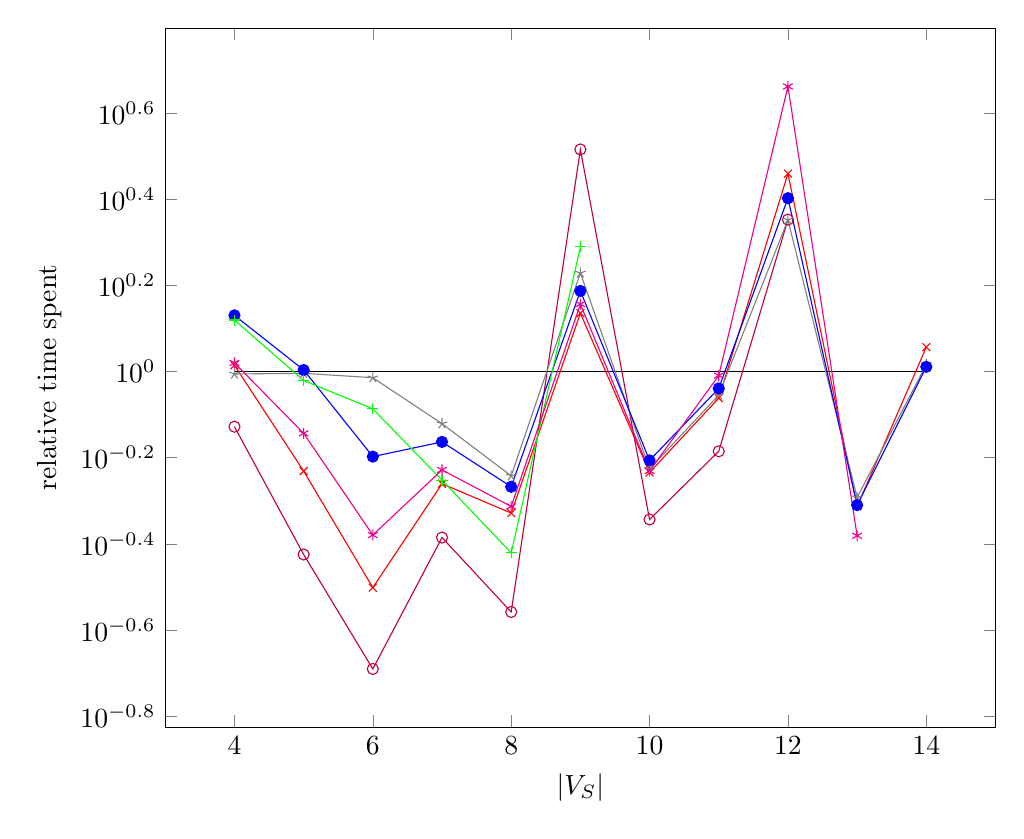
\begin{tikzpicture}
    \begin{axis}[
        xlabel=$|V_S|$,
        ylabel=relative time spent,
        ymode=log,
        legend style={at={(0.9,0.1)},anchor=south east},
        width=\textwidth,
		y tick label style={/pgf/number format/sci},
    ]
\addplot [mark=none, black] plot coordinates {
        (4,1) (14, 1)};



\addplot[
        mark=x,
        red,
    ] plot coordinates {
        (4,1.0341963936340537)
        (5,0.5872212498317262)
        (6,0.3150252343592421)
        (7,0.5489328540502025)
        (8,0.4691563660507788)
        (9,1.3659267214920254)
        (10,0.5829158055427053)
        (11,0.8675410228213514)
        (12,2.8804215346851567)
        (13,0.48622042850802205)
        (14,1.139249103225921)
};
%    \addlegendentry{DFS}


\addplot[
        mark=o,
        purple,
    ] plot coordinates {
        (4,0.7446160731342548)
        (5,0.3760872484757529)
        (6,0.20395691063619348)
        (7,0.4116723120141347)
        (8,0.2765761366043523)
        (9,3.277702486377702)
        (10,0.45345557621451693)
        (11,0.6529131347050375)
        (12,2.253102642969394)
};
%    \addlegendentry{GDFS O IP}


\addplot[
        mark=star,
        gray,
    ] plot coordinates {
        (4,0.986998285923268)
        (5,0.990456016904658)
        (6,0.9676159305638337)
        (7,0.7569661999435013)
        (8,0.5726394480903727)
        (9,1.6935978244098564)
        (10,0.5939935948858152)
        (11,0.8819548932880411)
        (12,2.250262287942807)
        (13,0.5098016055539938)
        (14,1.0382537813550197)
};
%    \addlegendentry{GDFS C}


\addplot[
        mark=*,
        blue,
    ] plot coordinates {
        (4,1.350280192589271)
        (5,1.0083990021448497)
        (6,0.6346349881535795)
        (7,0.6865130883699138)
        (8,0.5401179927275145)
        (9,1.5384974483498595)
        (10,0.6218905966067542)
        (11,0.9136191743894921)
        (12,2.5263424220943915)
        (13,0.4895304853304312)
        (14,1.025493765853684)
};
%    \addlegendentry{K-Path}


\addplot[
        mark=+,
        green,
    ] plot coordinates {
        (4,1.316795353041837)
        (5,0.9532402532500417)
        (6,0.8191487199612747)
        (7,0.5596281163603946)
        (8,0.3792225987672416)
        (9,1.9471981919246635)
};
%    \addlegendentry{CP}


\addplot[
        mark=asterisk,
        magenta,
    ] plot coordinates {
        (4,1.0472612442074125)
        (5,0.718669879592718)
        (6,0.4172863346749811)
        (7,0.5909828175058394)
        (8,0.48615922809785606)
        (9,1.4337866356743774)
        (10,0.5877303758542455)
        (11,0.9788108288373746)
        (12,4.589963118304846)
        (13,0.4155118413601153)
};
%    \addlegendentry{GDFS A IP}

	
	
    \end{axis}
    \end{tikzpicture}

\caption{cached}

\end{subfigure}\\[1ex]
\begin{subfigure}{0.5\linewidth}
\centering

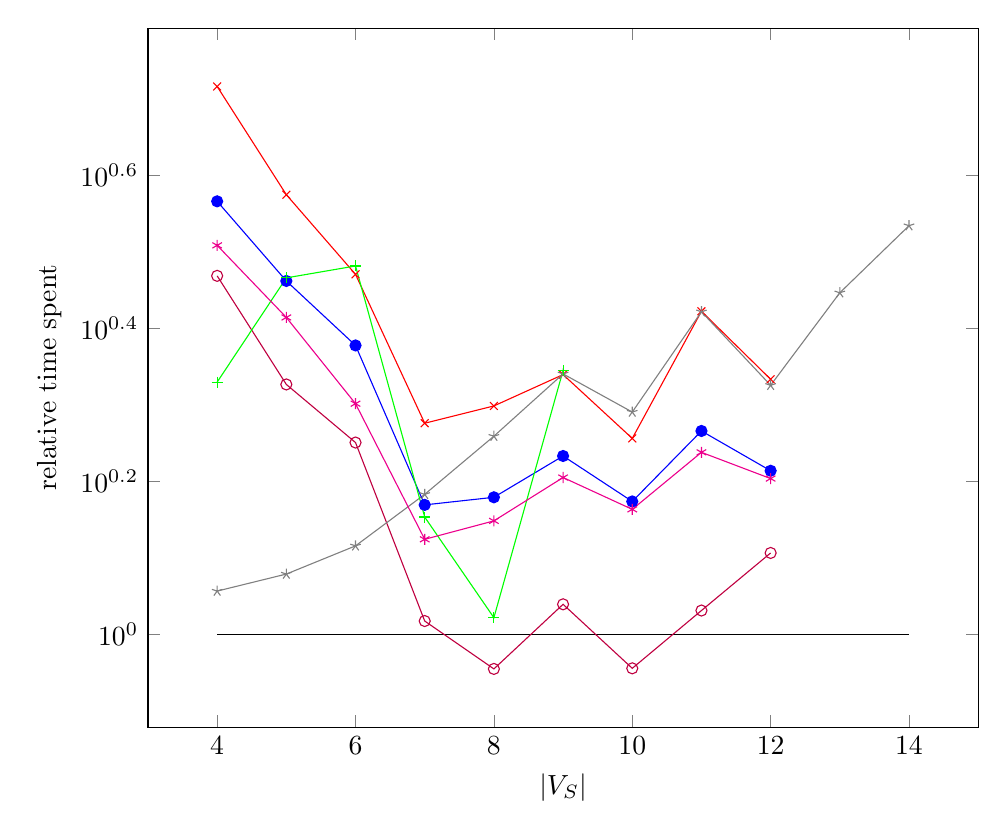
\begin{tikzpicture}
    \begin{axis}[
        xlabel=$|V_S|$,
        ylabel=relative time spent,
        ymode=log,
        legend style={at={(0.9,0.1)},anchor=south east},
        width=\textwidth,
		y tick label style={/pgf/number format/sci},
    ]
\addplot [mark=none, black] plot coordinates {
        (4,1) (14, 1)};



\addplot[
        mark=x,
        red,
    ] plot coordinates {
        (4,5.202946551261944)
        (5,3.756162046192574)
        (6,2.9549254023879072)
        (7,1.8872742557474473)
        (8,1.9880582223277101)
        (9,2.1847812854733193)
        (10,1.8028559351037163)
        (11,2.6436531391416507)
        (12,2.1539273359082483)
};
%    \addlegendentry{DFS}


\addplot[
        mark=o,
        purple,
    ] plot coordinates {
        (4,2.9414858115997387)
        (5,2.120863031356877)
        (6,1.7804930224229873)
        (7,1.0400701807728874)
        (8,0.9003554054490217)
        (9,1.0937936596519373)
        (10,0.9019831415298204)
        (11,1.0734764108654673)
        (12,1.2767276824510232)
};
%    \addlegendentry{GDFS O IP}


\addplot[
        mark=star,
        gray,
    ] plot coordinates {
        (4,1.1382355278673217)
        (5,1.198063456290179)
        (6,1.3042425098741526)
        (7,1.5233183009320665)
        (8,1.8148828000886499)
        (9,2.189451318312936)
        (10,1.9518249758925157)
        (11,2.639768817120566)
        (12,2.1154918845964863)
        (13,2.7952098947822313)
        (14,3.4210781907374623)
};
%    \addlegendentry{GDFS C}


\addplot[
        mark=*,
        blue,
    ] plot coordinates {
        (4,3.6819210072894446)
        (5,2.896400619358773)
        (6,2.3852188316658136)
        (7,1.4756755823523737)
        (8,1.5098085945063882)
        (9,1.7097753943529064)
        (10,1.490937989140139)
        (11,1.8438583447137513)
        (12,1.635315159939935)
};
%    \addlegendentry{K-Path}


\addplot[
        mark=+,
        green,
    ] plot coordinates {
        (4,2.1359021980392736)
        (5,2.923428609692478)
        (6,3.0304568963312812)
        (7,1.4225695726266137)
        (8,1.0506565420981449)
        (9,2.212314905046649)
};
%    \addlegendentry{CP}


\addplot[
        mark=asterisk,
        magenta,
    ] plot coordinates {
        (4,3.2242822734185275)
        (5,2.5950345747500103)
        (6,2.0014242504647624)
        (7,1.3303134982815363)
        (8,1.4062726411755775)
        (9,1.6024494454371436)
        (10,1.4559250035524376)
        (11,1.7288683972843149)
        (12,1.5973164420401704)
};
%    \addlegendentry{GDFS A IP}

	
    \end{axis}
    \end{tikzpicture}

\caption{parallel}

\end{subfigure}
\begin{subfigure} {0.5\linewidth}
\centering

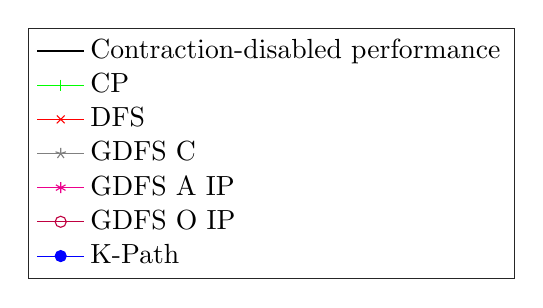
\begin{tikzpicture} 
    \begin{axis}[%
    hide axis,
    xmin=10,
    xmax=50,
    ymin=0,
    ymax=0.4,
    legend style={draw=white!15!black,legend cell align=left}
    ]
	\addlegendimage{black}
    \addlegendentry{Contraction-disabled performance}; 
     
    \addlegendimage{green, mark=+}
    \addlegendentry{CP};
    
    \addlegendimage{red, mark=x}
    \addlegendentry{DFS};
    
    \addlegendimage{gray, mark=star}
    \addlegendentry{GDFS C};
    
    \addlegendimage{magenta, mark=asterisk}
    \addlegendentry{GDFS A IP};
    
    \addlegendimage{purple, mark=o}
    \addlegendentry{GDFS O IP};
    
    \addlegendimage{blue, mark=*}
    \addlegendentry{K-Path};
    
    \end{axis}
\end{tikzpicture}

\end{subfigure}

\caption{Performance of our algorithm with \textbf{ZeroDomain} pruning using \textbf{`N-Filtering'} filtering relative to the performance of the algorithm without pruning. We avoid unnecessarily long paths, do not perform contraction and use the degree-based target graph vertex ordering. Data points above the black reference line denote that the pruning method introduces more delay, and data points below the reference line denote that the pruning method saves time. Note the logarithmic y-axis.}	
\label{fig:zerodomainnfiltering}
\end{figure}




\begin{figure}
\begin{subfigure}{.5\linewidth}
\centering

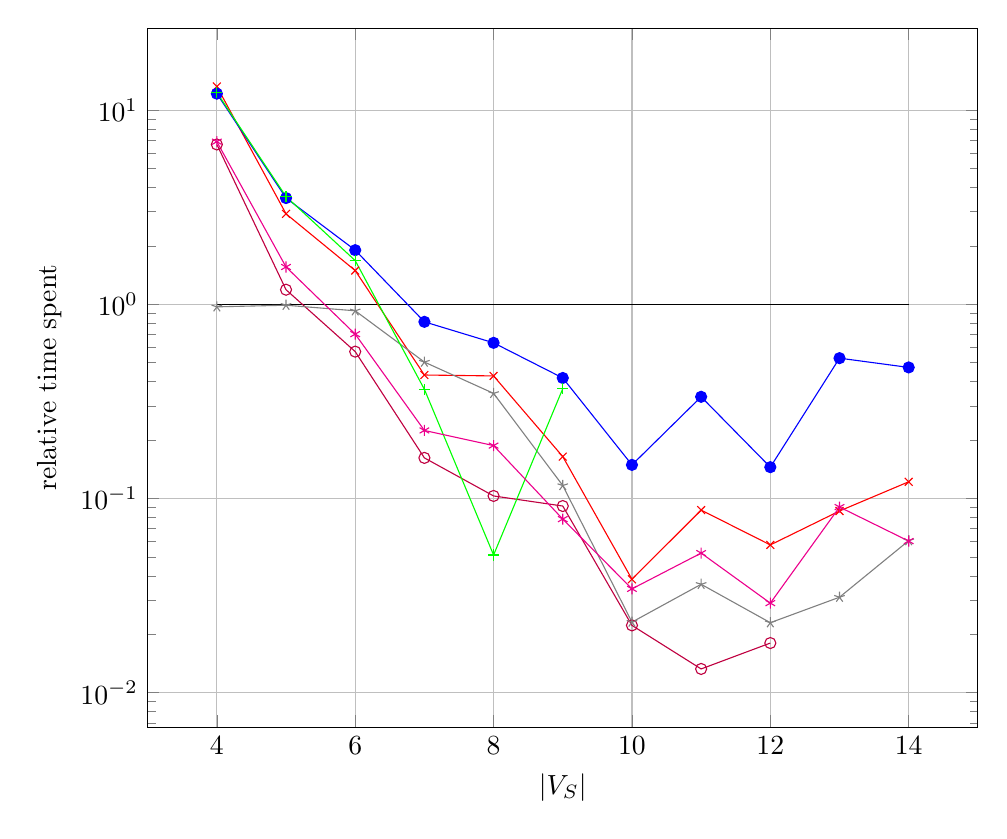
\begin{tikzpicture}
    \begin{axis}[
        xlabel=$|V_S|$,
        ylabel=relative time spent,
        ymode=log,
        legend style={at={(0.9,0.1)},anchor=south east},
        width=\textwidth,
		y tick label style={/pgf/number format/sci},
        ymajorgrids,
        xmajorgrids,		
    ]
\addplot [mark=none, black] plot coordinates {
        (4,1) (14, 1)};

    
	

\addplot[
        mark=x,
        red,
    ] plot coordinates {
        (4,13.228536748772864)
        (5,2.923043265236232)
        (6,1.4918465046685692)
        (7,0.43251422608381307)
        (8,0.4278138461953538)
        (9,0.1643974532055621)
        (10,0.0384235218883735)
        (11,0.08720339702951019)
        (12,0.05769871433439522)
        (13,0.08626318052038495)
        (14,0.12196687793734029)
};
%    \addlegendentry{DFS}


\addplot[
        mark=o,
        purple,
    ] plot coordinates {
        (4,6.652084765296219)
        (5,1.1887666847267304)
        (6,0.5706904469839822)
        (7,0.1619203743990465)
        (8,0.10311284594841497)
        (9,0.09148726872328639)
        (10,0.02222929883828284)
        (11,0.013264269229998682)
        (12,0.01803108077997606)
};
%    \addlegendentry{GDFS O IP}


\addplot[
        mark=star,
        gray,
    ] plot coordinates {
        (4,0.9704520516781957)
        (5,0.9891315449448252)
        (6,0.9259991321183858)
        (7,0.5041146272686665)
        (8,0.34789464456875185)
        (9,0.11668758068736773)
        (10,0.023108258037857765)
        (11,0.03619415549870497)
        (12,0.022948727466520213)
        (13,0.031049777535341994)
        (14,0.06069360971979865)
};
%    \addlegendentry{GDFS C}


\addplot[
        mark=*,
        blue,
    ] plot coordinates {
        (4,12.149621156018027)
        (5,3.524039042210963)
        (6,1.9000540945545796)
        (7,0.8124353858557827)
        (8,0.6333558749485183)
        (9,0.4176331133841372)
        (10,0.1490144308922331)
        (11,0.33404804566046264)
        (12,0.14504260141405623)
        (13,0.5281107544448288)
        (14,0.4731679498288802)
};
%    \addlegendentry{K-Path}


\addplot[
        mark=+,
        green,
    ] plot coordinates {
        (4,12.32026911652997)
        (5,3.58755573944772)
        (6,1.6790110096274846)
        (7,0.36496009660452833)
        (8,0.05120848928373445)
        (9,0.3680142027878651)
};
%    \addlegendentry{CP}


\addplot[
        mark=asterisk,
        magenta,
    ] plot coordinates {
        (4,6.876029334720606)
        (5,1.556841256929411)
        (6,0.7022607700874779)
        (7,0.22412843275278505)
        (8,0.18733394302820017)
        (9,0.07837119253519409)
        (10,0.03427027564684937)
        (11,0.05237617390308613)
        (12,0.028947697493439506)
        (13,0.09038890815957701)
        (14,0.0604047187048502)
};
%    \addlegendentry{GDFS A IP}
  
   
   
   

    \end{axis}
    \end{tikzpicture}


\caption{serial}

\end{subfigure}%
\begin{subfigure}{.5\linewidth}
\centering

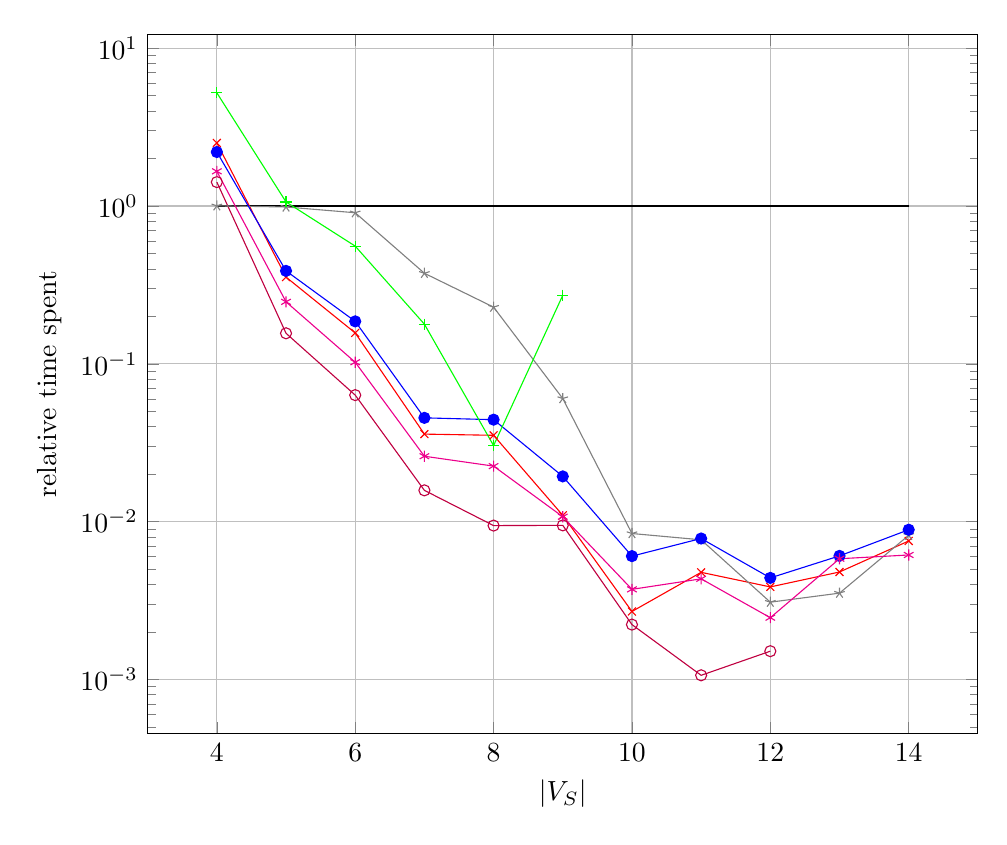
\begin{tikzpicture}
    \begin{axis}[
        xlabel=$|V_S|$,
        ylabel=relative time spent,
        ymode=log,
        legend style={at={(0.9,0.1)},anchor=south east},
        width=\textwidth,
		y tick label style={/pgf/number format/sci},
        ymajorgrids,
        xmajorgrids,		
    ]
\addplot [mark=none, black] plot coordinates {
        (4,1) (14, 1)};



\addplot[
        mark=x,
        red,
    ] plot coordinates {
        (4,2.5098178926779067)
        (5,0.3542854427484565)
        (6,0.15689010926635982)
        (7,0.035853449977087615)
        (8,0.03523223883158477)
        (9,0.010964699575333747)
        (10,0.0026948377810716018)
        (11,0.0047722023475749165)
        (12,0.003857850717237876)
        (13,0.0047953458790988)
        (14,0.007540380523948009)
};
%    \addlegendentry{DFS}


\addplot[
        mark=o,
        purple,
    ] plot coordinates {
        (4,1.4173101034075382)
        (5,0.1560990152619649)
        (6,0.06332634097438505)
        (7,0.0157805848059952)
        (8,0.009438491623514178)
        (9,0.009468907924155778)
        (10,0.002226287610086919)
        (11,0.001062190759533732)
        (12,0.0015102350651220453)
};
%    \addlegendentry{GDFS O IP}


\addplot[
        mark=star,
        gray,
    ] plot coordinates {
        (4,1.002529859429505)
        (5,0.9854105159518796)
        (6,0.906087246903251)
        (7,0.3747194523117736)
        (8,0.22865139116910282)
        (9,0.060236499046310454)
        (10,0.00840605207241163)
        (11,0.0076697916371780694)
        (12,0.003087366357886867)
        (13,0.003523082302813507)
        (14,0.008191107040264711)
};
%    \addlegendentry{GDFS C}


\addplot[
        mark=*,
        blue,
    ] plot coordinates {
        (4,2.1976489735425813)
        (5,0.3879928825633856)
        (6,0.18575151663949174)
        (7,0.0454443516390044)
        (8,0.044259974145741565)
        (9,0.01934413411554503)
        (10,0.006044262197985706)
        (11,0.007817157760072191)
        (12,0.004400728544806665)
        (13,0.0060658785631791945)
        (14,0.008884903299891778)
};
%    \addlegendentry{K-Path}


\addplot[
        mark=+,
        green,
    ] plot coordinates {
        (4,5.210336306845926)
        (5,1.0605278688734023)
        (6,0.5567531798646309)
        (7,0.17832988212555723)
        (8,0.03032795503714869)
        (9,0.2717523415218701)
};
%    \addlegendentry{CP}


\addplot[
        mark=asterisk,
        magenta,
    ] plot coordinates {
        (4,1.6585184570290825)
        (5,0.24696367603814495)
        (6,0.102320267871855)
        (7,0.025963378720697206)
        (8,0.02247569274863903)
        (9,0.010741035240163122)
        (10,0.003723269579006816)
        (11,0.004340017423267284)
        (12,0.0024617244953977213)
        (13,0.0058187731897781925)
        (14,0.006146499125306626)
};
%    \addlegendentry{GDFS A IP}

	
    \end{axis}
    \end{tikzpicture}

\caption{cached}

\end{subfigure}\\[1ex]
\begin{subfigure}{0.5\linewidth}
\centering

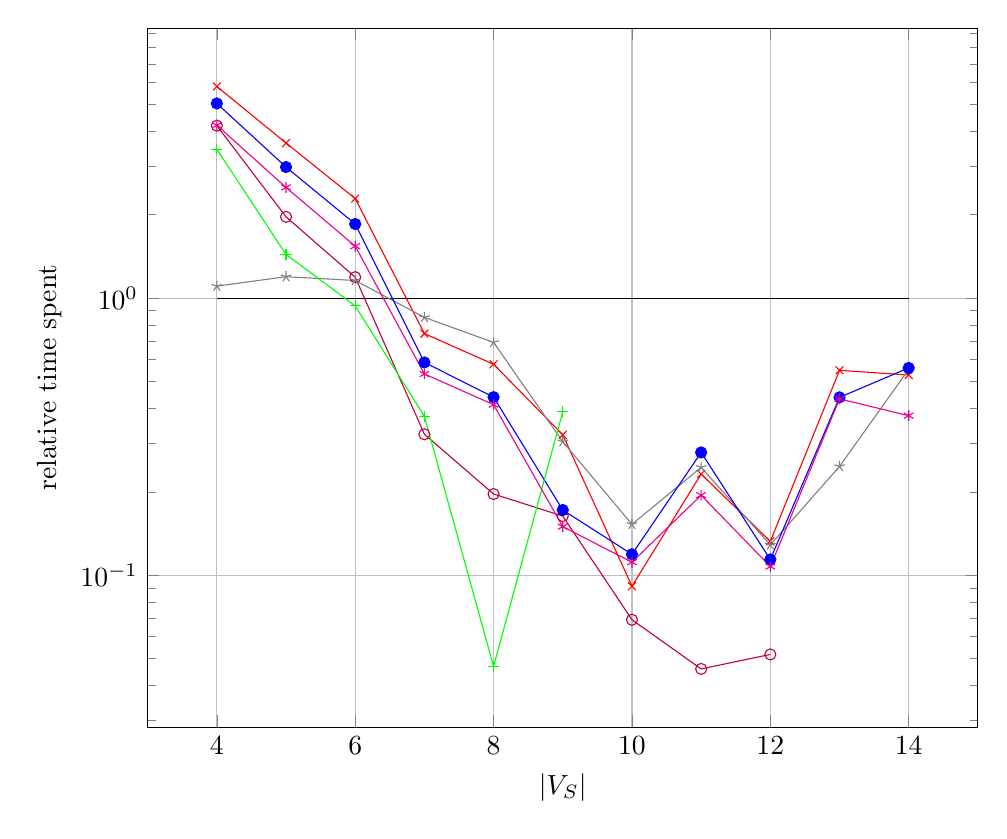
\begin{tikzpicture}
    \begin{axis}[
        xlabel=$|V_S|$,
        ylabel=relative time spent,
        ymode=log,
        legend style={at={(0.9,0.1)},anchor=south east},
        width=\textwidth,
		y tick label style={/pgf/number format/sci},
        ymajorgrids,
        xmajorgrids,		
    ]
\addplot [mark=none, black] plot coordinates {
        (4,1) (14, 1)};



\addplot[
        mark=x,
        red,
    ] plot coordinates {
        (4,5.798792679850153)
        (5,3.6257004403518205)
        (6,2.285202142417693)
        (7,0.7445129848838659)
        (8,0.5770188169893984)
        (9,0.3210938826132116)
        (10,0.09131787739629149)
        (11,0.23183733254071692)
        (12,0.13250978599133645)
        (13,0.5487572087616573)
        (14,0.5277236677256409)
};
%    \addlegendentry{DFS}


\addplot[
        mark=o,
        purple,
    ] plot coordinates {
        (4,4.1869563644643)
        (5,1.963563805539359)
        (6,1.1893882290176945)
        (7,0.3225915596294)
        (8,0.196417660886969)
        (9,0.1635088016201688)
        (10,0.06910862435318588)
        (11,0.045930260406800816)
        (12,0.0518105433910061)
};
%    \addlegendentry{GDFS O IP}


\addplot[
        mark=star,
        gray,
    ] plot coordinates {
        (4,1.1043656381381906)
        (5,1.1941146142677403)
        (6,1.1571769969713963)
        (7,0.8519147110949141)
        (8,0.6919890069549386)
        (9,0.30329744854481366)
        (10,0.15267006969696184)
        (11,0.2451122958148758)
        (12,0.12868565849738745)
        (13,0.2468665194487868)
        (14,0.5529525262522433)
};
%    \addlegendentry{GDFS C}


\addplot[
        mark=*,
        blue,
    ] plot coordinates {
        (4,5.036262260510419)
        (5,2.969188933770786)
        (6,1.8496830497872034)
        (7,0.5859718273323613)
        (8,0.43912493395440744)
        (9,0.17191408110115602)
        (10,0.11902810316960899)
        (11,0.2773735237523154)
        (12,0.114049211518233)
        (13,0.438365362697428)
        (14,0.5597451487697097)
};
%    \addlegendentry{K-Path}


\addplot[
        mark=+,
        green,
    ] plot coordinates {
        (4,3.4404078593966663)
        (5,1.4365332891311595)
        (6,0.9370666124380356)
        (7,0.37433319924673136)
        (8,0.04688253357281991)
        (9,0.38910890933793285)
};
%    \addlegendentry{CP}


\addplot[
        mark=asterisk,
        magenta,
    ] plot coordinates {
        (4,4.202135993006676)
        (5,2.5066991227985915)
        (6,1.5392306053079454)
        (7,0.5323918363219251)
        (8,0.41254854061922086)
        (9,0.14979269284608565)
        (10,0.11144241399443222)
        (11,0.1944784771207959)
        (12,0.10750387177004295)
        (13,0.43288906698477536)
        (14,0.37647551651848066)
};
%    \addlegendentry{GDFS A IP}

	
    \end{axis}
    \end{tikzpicture}

\caption{parallel}

\end{subfigure}
\begin{subfigure} {0.5\linewidth}
\centering

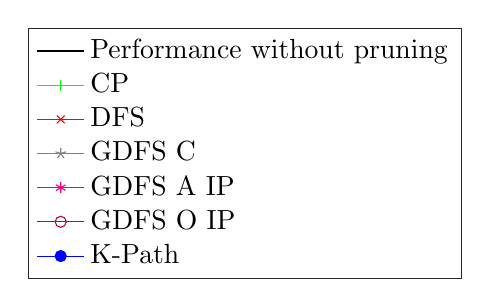
\begin{tikzpicture} 
    \begin{axis}[%
    hide axis,
    xmin=10,
    xmax=50,
    ymin=0,
    ymax=0.4,
    legend style={draw=white!15!black,legend cell align=left}
    ]
	\addlegendimage{black}
    \addlegendentry{Performance without pruning}; 
     
    \addlegendimage{green, mark=+}
    \addlegendentry{CP};
    
    \addlegendimage{red, mark=x}
    \addlegendentry{DFS};
    
    \addlegendimage{gray, mark=star}
    \addlegendentry{GDFS C};
    
    \addlegendimage{magenta, mark=asterisk}
    \addlegendentry{GDFS A IP};
    
    \addlegendimage{purple, mark=o}
    \addlegendentry{GDFS O IP};
    
    \addlegendimage{blue, mark=*}
    \addlegendentry{K-Path};
    
    \end{axis}
\end{tikzpicture}

\end{subfigure}

\caption{Performance of our algorithm with \textbf{AllDifferent} pruning using \textbf{`Labels and neighbours'} filtering relative to the performance of the algorithm without pruning. $|V_T|=1\frac{1}{2}*|V_S|$, ``refuse longer paths" and contraction are disabled and we use the degree-based target graph vertex ordering. Data points above the black reference line denote that the pruning method introduces more delay, and data points below the reference line denote that the pruning method saves time. Note the logarithmic y-axis.}	
\label{fig:alldifferentlabelsneighbours}
\end{figure}


\begin{figure}
\begin{subfigure}{.5\linewidth}
\centering

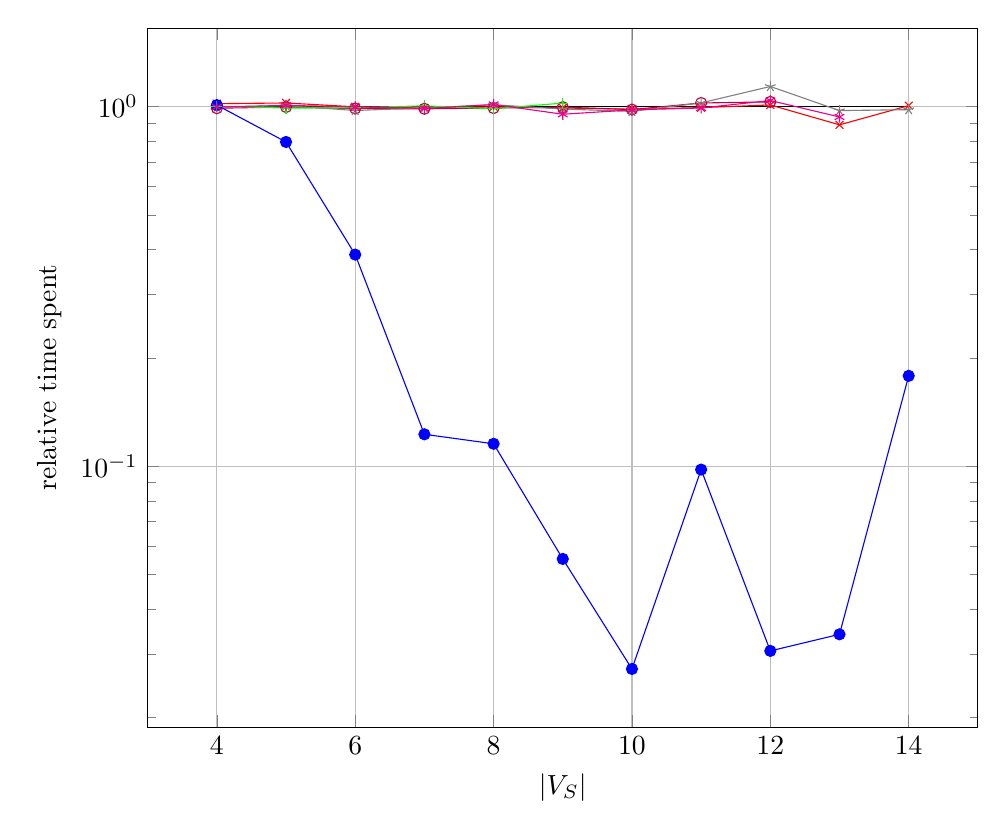
\begin{tikzpicture}
    \begin{axis}[
        xlabel=$|V_S|$,
        ylabel=relative time spent,
        ymode=log,
        legend style={at={(0.9,0.1)},anchor=south east},
        width=\textwidth,
		y tick label style={/pgf/number format/sci},
        ymajorgrids,
        xmajorgrids,		
    ]
\addplot [mark=none, black] plot coordinates {
        (4,1) (14, 1)};

    
   

\addplot[
        mark=x,
        red,
    ] plot coordinates {
        (4,1.0186997833347926)
        (5,1.0232045351532169)
        (6,0.9983077611450746)
        (7,0.9907049947363294)
        (8,0.9986106752415018)
        (9,0.990947997808037)
        (10,0.9833582387420912)
        (11,0.9932844129587108)
        (12,1.0103133629860612)
        (13,0.8895477690842722)
        (14,1.005905267592158)
};
%    \addlegendentry{DFS}


\addplot[
        mark=o,
        purple,
    ] plot coordinates {
        (4,0.9894734471098923)
        (5,0.9968820127769855)
        (6,0.9873225419658352)
        (7,0.9858166681275962)
        (8,0.9904807801930379)
        (9,0.996328709955975)
        (10,0.9809044726735501)
        (11,1.0231407177222254)
        (12,1.0305198945131373)
};
%    \addlegendentry{GDFS O IP}


\addplot[
        mark=star,
        gray,
    ] plot coordinates {
        (4,0.9951732111609184)
        (5,1.005781000751052)
        (6,0.9751302373376524)
        (7,0.9914699309037306)
        (8,1.011362037912515)
        (9,0.9843712362591021)
        (10,0.969402089834849)
        (11,1.0237476067658449)
        (12,1.137294643132325)
        (13,0.9744371513907365)
        (14,0.9802787976693997)
};
%    \addlegendentry{GDFS C}


\addplot[
        mark=*,
        blue,
    ] plot coordinates {
        (4,1.0092933808186613)
        (5,0.7972700999022878)
        (6,0.3874509873372779)
        (7,0.12257854741680918)
        (8,0.11535787568739275)
        (9,0.05517912995992491)
        (10,0.027274471216057083)
        (11,0.09778018796630517)
        (12,0.030614788275003413)
        (13,0.03405177172923535)
        (14,0.17825871037578678)
};
%    \addlegendentry{K-Path}


\addplot[
        mark=+,
        green,
    ] plot coordinates {
        (4,1.0028356859109526)
        (5,0.9904361969575739)
        (6,0.9923987001325429)
        (7,1.0046817332100164)
        (8,0.9858188647918942)
        (9,1.0225063689622522)
};
%    \addlegendentry{CP}


\addplot[
        mark=asterisk,
        magenta,
    ] plot coordinates {
        (4,0.9976349962184932)
        (5,1.0073844165930093)
        (6,0.9981453884688307)
        (7,0.9876792768127225)
        (8,1.0133814377011994)
        (9,0.9520147690376894)
        (10,0.9790339992527488)
        (11,0.9908681483629362)
        (12,1.039543646663335)
        (13,0.9354622696539593)
};
%    \addlegendentry{GDFS A IP}


    \end{axis}
    \end{tikzpicture}


\caption{serial}

\end{subfigure}%
\begin{subfigure}{.5\linewidth}
\centering

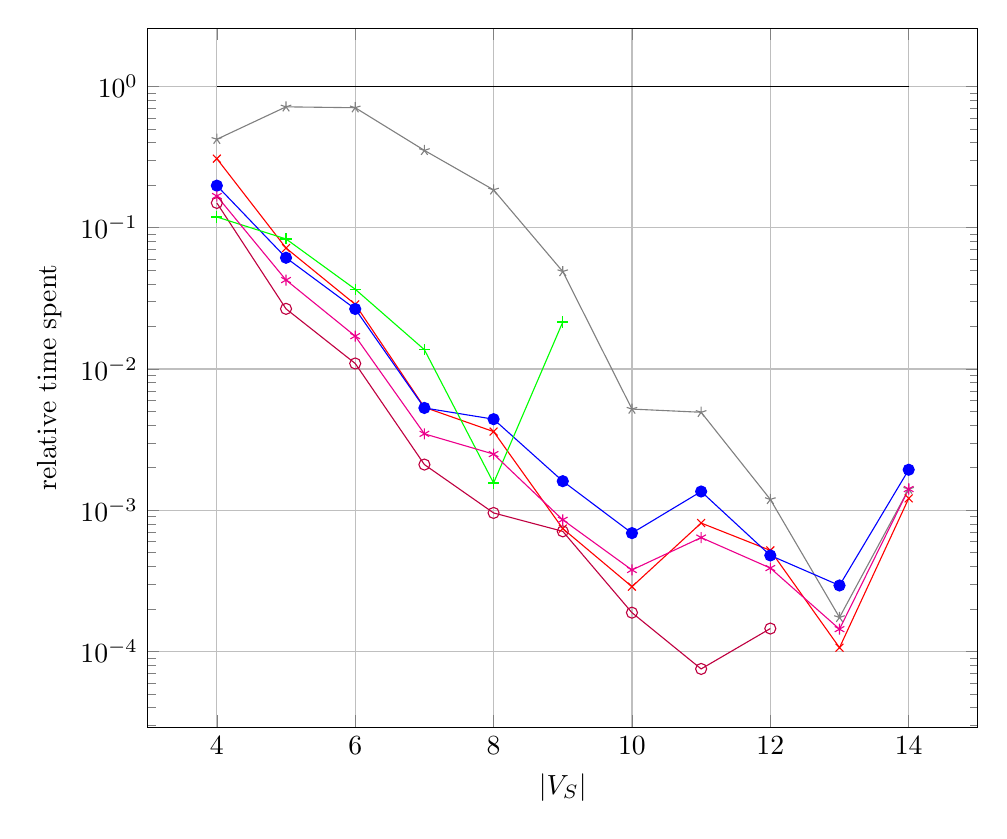
\begin{tikzpicture}
    \begin{axis}[
        xlabel=$|V_S|$,
        ylabel=relative time spent,
        ymode=log,
        legend style={at={(0.9,0.1)},anchor=south east},
        width=\textwidth,
		y tick label style={/pgf/number format/sci},
        ymajorgrids,
        xmajorgrids,		
    ]
\addplot [mark=none, black] plot coordinates {
        (4,1) (14, 1)};


	

\addplot[
        mark=x,
        red,
    ] plot coordinates {
        (4,0.3083735334423767)
        (5,0.0717983121165574)
        (6,0.02867174161124386)
        (7,0.005353932759145197)
        (8,0.0036018766107605016)
        (9,7.415681550873021E-4)
        (10,2.875045828804046E-4)
        (11,8.113057744684182E-4)
        (12,5.194226380311751E-4)
        (13,1.0634101119189054E-4)
        (14,0.0012129348920926208)
};
%    \addlegendentry{DFS}


\addplot[
        mark=o,
        purple,
    ] plot coordinates {
        (4,0.14979438676735934)
        (5,0.026646145040194358)
        (6,0.010934376147201053)
        (7,0.0021043263511895116)
        (8,9.565212575048943E-4)
        (9,7.087506618627115E-4)
        (10,1.8824424486718616E-4)
        (11,7.522826832084828E-5)
        (12,1.452779418016359E-4)
};
%    \addlegendentry{GDFS O IP}


\addplot[
        mark=star,
        gray,
    ] plot coordinates {
        (4,0.42295684080525053)
        (5,0.7175652095808638)
        (6,0.7072294111057362)
        (7,0.3528461610206276)
        (8,0.1853565026591184)
        (9,0.04895326827559776)
        (10,0.00520061691970819)
        (11,0.004936257731941951)
        (12,0.001192029881315615)
        (13,1.741539188091501E-4)
        (14,0.0014103432783372227)
};
%    \addlegendentry{GDFS C}


\addplot[
        mark=*,
        blue,
    ] plot coordinates {
        (4,0.19863010172526796)
        (5,0.06127991045420755)
        (6,0.02659926027389259)
        (7,0.005297029257396946)
        (8,0.004410971673992958)
        (9,0.0016052971971944885)
        (10,6.884416663917037E-4)
        (11,0.0013566163358025296)
        (12,4.784200055767407E-4)
        (13,2.932097067133155E-4)
        (14,0.0019350025642613788)
};
%    \addlegendentry{K-Path}


\addplot[
        mark=+,
        green,
    ] plot coordinates {
        (4,0.11914885358071148)
        (5,0.08325890354708809)
        (6,0.03669565157098442)
        (7,0.013693561308514623)
        (8,0.0015581760794368682)
        (9,0.021493389120216477)
};
%    \addlegendentry{CP}


\addplot[
        mark=asterisk,
        magenta,
    ] plot coordinates {
        (4,0.167629941635991)
        (5,0.04261429975714803)
        (6,0.01708358998028725)
        (7,0.0034731132709504564)
        (8,0.0024963114206875137)
        (9,8.552890640062261E-4)
        (10,3.776131025451379E-4)
        (11,6.400771612525835E-4)
        (12,3.8951787719665454E-4)
        (13,1.4388024718858805E-4)
        (14,0.0014124109249871175)
};
%    \addlegendentry{GDFS A IP}

	
    \end{axis}
    \end{tikzpicture}

\caption{cached}

\end{subfigure}\\[1ex]
\begin{subfigure}{0.5\linewidth}
\centering

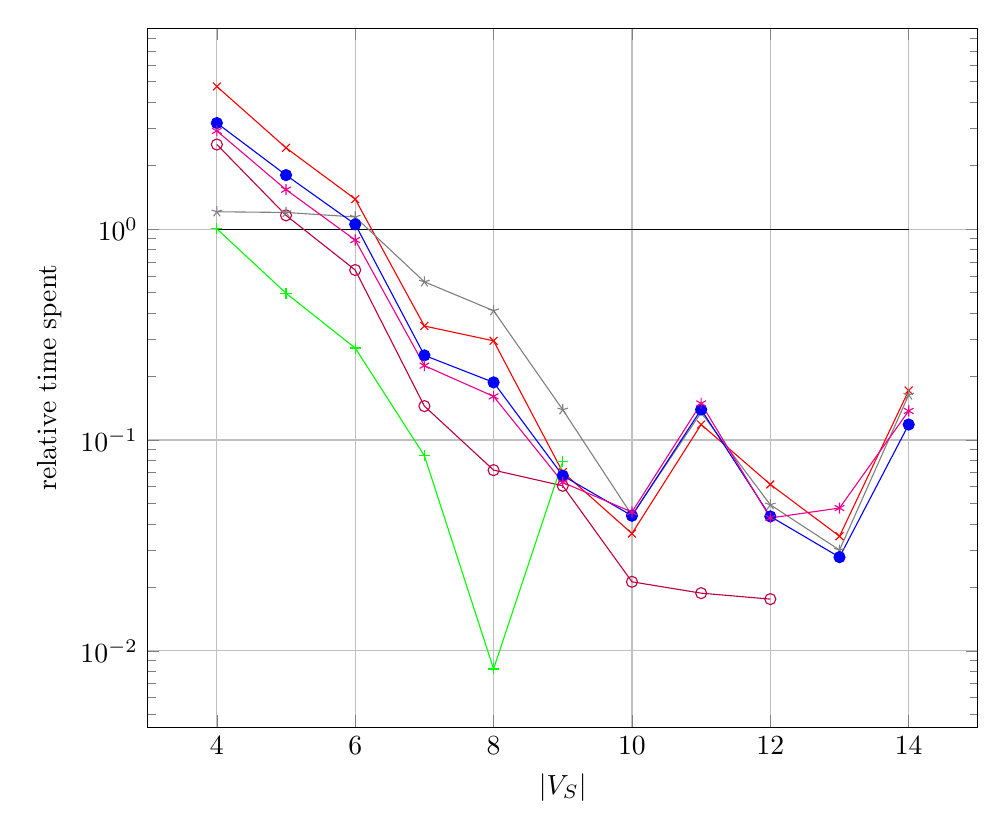
\begin{tikzpicture}
    \begin{axis}[
        xlabel=$|V_S|$,
        ylabel=relative time spent,
        ymode=log,
        legend style={at={(0.9,0.1)},anchor=south east},
        width=\textwidth,
		y tick label style={/pgf/number format/sci},
        ymajorgrids,
        xmajorgrids,		
    ]
\addplot [mark=none, black] plot coordinates {
        (4,1) (14, 1)};



\addplot[
        mark=x,
        red,
    ] plot coordinates {
        (4,4.748759594123889)
        (5,2.4295540762796515)
        (6,1.3875324748809377)
        (7,0.3470734386774885)
        (8,0.2952023716844192)
        (9,0.0703958686196079)
        (10,0.03598320014357281)
        (11,0.1183808662884438)
        (12,0.06153628532584232)
        (13,0.03494338911404371)
        (14,0.17160278085125824)
};
%    \addlegendentry{DFS}


\addplot[
        mark=o,
        purple,
    ] plot coordinates {
        (4,2.519594921852216)
        (5,1.1621656243183787)
        (6,0.6397718531506256)
        (7,0.14471136627669023)
        (8,0.07193325075024548)
        (9,0.0605941046017171)
        (10,0.021240531171245025)
        (11,0.018767566782790235)
        (12,0.01758393553367299)
};
%    \addlegendentry{GDFS O IP}


\addplot[
        mark=star,
        gray,
    ] plot coordinates {
        (4,1.2087512038670705)
        (5,1.1995330941514946)
        (6,1.1418853789726933)
        (7,0.5621877889562694)
        (8,0.41022833627945976)
        (9,0.13903913868573037)
        (10,0.04393563116464705)
        (11,0.13498526740722694)
        (12,0.049268960174921994)
        (13,0.030051623484468215)
        (14,0.1635365740440703)
};
%    \addlegendentry{GDFS C}


\addplot[
        mark=*,
        blue,
    ] plot coordinates {
        (4,3.1851467361084174)
        (5,1.8038765225341042)
        (6,1.0539452554077893)
        (7,0.2518608123839957)
        (8,0.18755266523230274)
        (9,0.06769612412018444)
        (10,0.043697519958703857)
        (11,0.1394520374224132)
        (12,0.04337870481595418)
        (13,0.02780400571582131)
        (14,0.11833494711833015)
};
%    \addlegendentry{K-Path}


\addplot[
        mark=+,
        green,
    ] plot coordinates {
        (4,1.0029463243603973)
        (5,0.49661067861132135)
        (6,0.27286554408201)
        (7,0.08419120306502847)
        (8,0.008199948214019814)
        (9,0.07911018316730134)
};
%    \addlegendentry{CP}


\addplot[
        mark=asterisk,
        magenta,
    ] plot coordinates {
        (4,2.92253226917892)
        (5,1.5385463516143498)
        (6,0.8879009793117698)
        (7,0.22506649596273964)
        (8,0.1609402158565465)
        (9,0.06290335332168706)
        (10,0.04548679530232991)
        (11,0.14892017614069342)
        (12,0.04266555665061478)
        (13,0.04753845861304018)
        (14,0.13727172289974587)
};
%    \addlegendentry{GDFS A IP}

	
    \end{axis}
    \end{tikzpicture}

\caption{parallel}

\end{subfigure}
\begin{subfigure} {0.5\linewidth}
\centering

\begin{tikzpicture} 
    \begin{axis}[%
    hide axis,
    xmin=10,
    xmax=50,
    ymin=0,
    ymax=0.4,
    legend style={draw=white!15!black,legend cell align=left}
    ]
	\addlegendimage{black}
    \addlegendentry{Performance without pruning}; 
     
    \addlegendimage{green, mark=+}
    \addlegendentry{CP};
    
    \addlegendimage{red, mark=x}
    \addlegendentry{DFS};
    
    \addlegendimage{gray, mark=star}
    \addlegendentry{GDFS C};
    
    \addlegendimage{magenta, mark=asterisk}
    \addlegendentry{GDFS A IP};
    
    \addlegendimage{purple, mark=o}
    \addlegendentry{GDFS O IP};
    
    \addlegendimage{blue, mark=*}
    \addlegendentry{K-Path};
    
    \end{axis}
\end{tikzpicture}

\end{subfigure}

\caption{Performance of our algorithm with \textbf{AllDifferent} pruning using \textbf{`Free neighbours'} filtering relative to the performance of the algorithm without pruning. $|V_T|=1\frac{1}{2}*|V_S|$, ``refuse longer paths" and contraction are disabled and we use the degree-based target graph vertex ordering. Data points above the black reference line denote that the pruning method introduces more delay, and data points below the reference line denote that the pruning method saves time. Note the logarithmic y-axis.}		
\label{fig:alldifferentunmatched}
\end{figure}


\begin{figure}
\begin{subfigure}{.5\linewidth}
\centering

\begin{tikzpicture}
    \begin{axis}[
        xlabel=$|V_S|$,
        ylabel=relative time spent,
        ymode=log,
        legend style={at={(0.9,0.1)},anchor=south east},
        width=\textwidth,
		y tick label style={/pgf/number format/sci},
    ]
\addplot [mark=none, black] plot coordinates {
        (4,1) (14, 1)};


\addplot[
        mark=x,
        red,
    ] plot coordinates {
        (4,0.9961858191755759)
        (5,1.0059848034836174)
        (6,1.0015623854405225)
        (7,1.0041850516247017)
        (8,0.992834292174954)
        (9,0.9805831782750661)
        (10,1.0131070860496907)
        (11,0.9820629029946675)
        (12,0.9731684469245409)
        (13,0.9978012338195624)
};
%    \addlegendentry{DFS}


\addplot[
        mark=o,
        purple,
    ] plot coordinates {
        (4,0.9991254113598864)
        (5,1.0006304793357408)
        (6,0.9997389129846505)
        (7,1.0024122661594037)
        (8,0.9960200414287358)
        (9,0.9797204693043249)
        (10,1.006094756978359)
        (11,1.0291250941127874)
        (12,1.016228045334132)
};
%    \addlegendentry{GDFS O IP}


\addplot[
        mark=star,
        gray,
    ] plot coordinates {
        (4,1.0059277991423625)
        (5,0.9907814973218768)
        (6,1.0243229749286393)
        (7,1.020235901218478)
        (8,1.028660392466402)
        (9,0.9992951555916159)
        (10,0.9825124885953094)
        (11,0.9832292458336007)
        (12,1.0260311821681063)
        (13,1.1015279814561096)
        (14,1.0152331060942739)
};
%    \addlegendentry{GDFS C}


\addplot[
        mark=*,
        blue,
    ] plot coordinates {
        (4,1.1428023873341047)
        (5,0.8363144144880936)
        (6,0.3883692600044063)
        (7,0.12306323448284873)
        (8,0.11750735154321501)
        (9,0.05546079701782758)
        (10,0.027198570773209862)
        (11,0.09188685028611088)
        (12,0.029187752530780098)
        (13,0.028763961047358233)
        (14,0.13514762161751237)
};
%    \addlegendentry{K-Path}


\addplot[
        mark=+,
        green,
    ] plot coordinates {
        (4,1.003240741424298)
        (5,1.0007002255334068)
        (6,0.9998134962523451)
        (7,0.9954368842322697)
        (8,0.9901138150986978)
        (9,1.0994301778756659)
};
%    \addlegendentry{CP}


\addplot[
        mark=asterisk,
        magenta,
    ] plot coordinates {
        (4,1.012208101549136)
        (5,1.004540535143729)
        (6,1.006238667112502)
        (7,0.9987787321626621)
        (8,0.9857632446293185)
        (9,1.00045313105658)
        (10,0.9800057859162024)
        (11,1.0071924078562504)
        (12,1.05284665552656)
        (13,1.0473613609958743)
};
%    \addlegendentry{GDFS A IP}

 

    \end{axis}
    \end{tikzpicture}


\caption{serial}

\end{subfigure}%
\begin{subfigure}{.5\linewidth}
\centering

\begin{tikzpicture}
        \begin{axis}[
        xlabel=$|V_S|$,
        ylabel=relative time spent,
        ymode=log,
        legend style={at={(0.9,0.1)},anchor=south east},
        width=\textwidth,
		y tick label style={/pgf/number format/sci},
    ]
\addplot [mark=none, black] plot coordinates {
        (4,1) (14, 1)};

	

\addplot[
        mark=x,
        red,
    ] plot coordinates {
        (4,0.28797946415268216)
        (5,0.07651582579324001)
        (6,0.0304666091954765)
        (7,0.005338589440600172)
        (8,0.0038271200815995776)
        (9,7.967244945263907E-4)
        (10,3.0777658183211987E-4)
        (11,7.316319897914259E-4)
        (12,3.4267518525965546E-4)
        (13,1.0795184070755415E-4)
        (14,7.623451601108666E-4)
};
%    \addlegendentry{DFS}


\addplot[
        mark=o,
        purple,
    ] plot coordinates {
        (4,0.15049515351200515)
        (5,0.028888664846084877)
        (6,0.011744849761370135)
        (7,0.0021597185405343167)
        (8,9.451813259466757E-4)
        (9,7.108005706910614E-4)
        (10,1.2347079460250932E-4)
        (11,9.95681216803268E-5)
        (12,1.6636754548371435E-4)
};
%    \addlegendentry{GDFS O IP}


\addplot[
        mark=star,
        gray,
    ] plot coordinates {
        (4,0.4261569662504955)
        (5,0.6566221486790923)
        (6,0.5577822930842058)
        (7,0.3218592258892897)
        (8,0.18912427965228307)
        (9,0.047186436624101824)
        (10,0.006370129606168451)
        (11,0.0012501421281951863)
        (12,0.001428282896214883)
        (13,1.4047897093971695E-4)
        (14,0.0012339028104273453)
};
%    \addlegendentry{GDFS C}


\addplot[
        mark=*,
        blue,
    ] plot coordinates {
        (4,0.19921889891317368)
        (5,0.06836073093997885)
        (6,0.02840796237713794)
        (7,0.005614455272937469)
        (8,0.004672519202561842)
        (9,0.001547859891521619)
        (10,4.269626026969231E-4)
        (11,0.0011715845435014138)
        (12,5.118613622622226E-4)
        (13,3.9341491023758834E-4)
        (14,0.0011207533086203814)
};
%    \addlegendentry{K-Path}


\addplot[
        mark=+,
        green,
    ] plot coordinates {
        (4,0.12065618974765957)
        (5,0.08159990593923339)
        (6,0.03466025100832615)
        (7,0.013147623578769863)
        (8,0.0017371671223744833)
        (9,0.03084198984204367)
};
%    \addlegendentry{CP}


\addplot[
        mark=asterisk,
        magenta,
    ] plot coordinates {
        (4,0.1784159199448806)
        (5,0.04687838004113365)
        (6,0.019250300262524056)
        (7,0.003877520221788777)
        (8,0.0028497378324052747)
        (9,9.238160016552532E-4)
        (10,3.1576391186238784E-4)
        (11,7.994265736620543E-4)
        (12,3.8594286429616265E-4)
        (13,1.6073739183641855E-4)
        (14,6.707501289580087E-4)
};
%    \addlegendentry{GDFS A IP}

	
    \end{axis}
    \end{tikzpicture}

\caption{cached}

\end{subfigure}\\[1ex]
\begin{subfigure}{0.5\linewidth}
\centering

\begin{tikzpicture}
    \begin{axis}[
        xlabel=$|V_S|$,
        ylabel=relative time spent,
        ymode=log,
        legend style={at={(0.9,0.1)},anchor=south east},
        width=\textwidth,
		y tick label style={/pgf/number format/sci},
    ]
\addplot [mark=none, black] plot coordinates {
        (4,1) (14, 1)};


\addplot[
        mark=x,
        red,
    ] plot coordinates {
        (4,3.9129439575545435)
        (5,2.273222753540935)
        (6,1.3358829167973778)
        (7,0.3060292392269831)
        (8,0.27310812493561054)
        (9,0.08483478635788988)
        (10,0.03220002459721227)
        (11,0.10965821877648596)
        (12,0.05238033266084752)
        (13,0.02720606162053374)
        (14,0.12326343330507006)
};
%    \addlegendentry{DFS}


\addplot[
        mark=o,
        purple,
    ] plot coordinates {
        (4,2.4370501012142824)
        (5,1.0568408408459573)
        (6,0.5835598718338068)
        (7,0.13489675395340783)
        (8,0.06428756573066419)
        (9,0.04934951432140211)
        (10,0.01966479503287344)
        (11,0.018929462405664066)
        (12,0.01752267312020006)
};
%    \addlegendentry{GDFS O IP}


\addplot[
        mark=star,
        gray,
    ] plot coordinates {
        (4,1.5119445424232758)
        (5,1.6205884547090093)
        (6,1.4772813435520415)
        (7,0.6353071431015811)
        (8,0.41070975405654797)
        (9,0.13580170759422583)
        (10,0.03828888536206054)
        (11,0.10934140002182946)
        (12,0.0411628308005999)
        (13,0.024956633661657346)
        (14,0.16725255988991872)
};
%    \addlegendentry{GDFS C}


\addplot[
        mark=*,
        blue,
    ] plot coordinates {
        (4,2.9292287176662284)
        (5,1.7085776030673339)
        (6,1.018144876988824)
        (7,0.22453968974110117)
        (8,0.18160614741581238)
        (9,0.06924099256113281)
        (10,0.04038867770933918)
        (11,0.12581531378172073)
        (12,0.04559446907724363)
        (13,0.04043070416472683)
        (14,0.10402774643082491)
};
%    \addlegendentry{K-Path}


\addplot[
        mark=+,
        green,
    ] plot coordinates {
        (4,0.9551312671725737)
        (5,0.46672792929157314)
        (6,0.25108420813909216)
        (7,0.09084564408241347)
        (8,0.009073128728892876)
        (9,0.09911792703918121)
};
%    \addlegendentry{CP}


\addplot[
        mark=asterisk,
        magenta,
    ] plot coordinates {
        (4,2.6450452172441703)
        (5,1.466590988138647)
        (6,0.8335425887125216)
        (7,0.20265590602141004)
        (8,0.14860699155681456)
        (9,0.058559839513090184)
        (10,0.03613722819737897)
        (11,0.1373961637320401)
        (12,0.039138601300597764)
        (13,0.04064207588686031)
        (14,0.09797085693851426)
};
%    \addlegendentry{GDFS A IP}

	
    \end{axis}
    \end{tikzpicture}

\caption{parallel}

\end{subfigure}
\begin{subfigure} {0.5\linewidth}
\centering

\begin{tikzpicture} 
    \begin{axis}[%
    hide axis,
    xmin=10,
    xmax=50,
    ymin=0,
    ymax=0.4,
    legend style={draw=white!15!black,legend cell align=left}
    ]
	\addlegendimage{black}
    \addlegendentry{Performance without pruning}; 
     
    \addlegendimage{green, mark=+}
    \addlegendentry{CP};
    
    \addlegendimage{red, mark=x}
    \addlegendentry{DFS};
    
    \addlegendimage{gray, mark=star}
    \addlegendentry{GDFS C};
    
    \addlegendimage{magenta, mark=asterisk}
    \addlegendentry{GDFS A IP};
    
    \addlegendimage{purple, mark=o}
    \addlegendentry{GDFS O IP};
    
    \addlegendimage{blue, mark=*}
    \addlegendentry{K-Path};
    
    \end{axis}
\end{tikzpicture}

\end{subfigure}

\caption{Performance of our algorithm with \textbf{AllDifferent} pruning using \textbf{`M-filtering'} filtering relative to the performance of the algorithm without pruning. We avoid unnecessarily long paths, do not perform contraction and use the degree-based target graph vertex ordering. Data points above the black reference line denote that the pruning method introduces more delay, and data points below the reference line denote that the pruning method saves time. Note the logarithmic y-axis.}		
\label{fig:alldifferentMfiltering}
\end{figure}


\begin{figure}
\begin{subfigure}{.5\linewidth}
\centering

\begin{tikzpicture}
    \begin{axis}[
        xlabel=$|V_S|$,
        ylabel=relative time spent,
        ymode=log,
        legend style={at={(0.9,0.1)},anchor=south east},
        width=\textwidth,
		y tick label style={/pgf/number format/sci},
    ]
\addplot [mark=none, black] plot coordinates {
        (4,1) (14,1)};

    
   

\addplot[
        mark=x,
        red,
    ] plot coordinates {
        (4,0.9676950624676575)
        (5,0.9988894067222226)
        (6,1.0005763973495974)
        (7,1.0012522076540606)
        (8,1.0107283953513952)
        (9,0.9599448767629568)
        (10,1.0347901686226628)
        (11,1.0103410684538925)
        (12,1.0255798438058548)
        (13,0.9056614547818025)
        (14,0.9698848854871277)
};
%    \addlegendentry{DFS}


\addplot[
        mark=o,
        purple,
    ] plot coordinates {
        (4,1.0094137822150915)
        (5,1.0030498615384387)
        (6,0.996041126474167)
        (7,1.0014862936237205)
        (8,1.006913278037861)
        (9,0.9865779317721944)
        (10,0.973979329150809)
        (11,1.0085691395261733)
        (12,1.012790208560442)
};
%    \addlegendentry{GDFS O IP}


\addplot[
        mark=star,
        gray,
    ] plot coordinates {
        (4,1.0410716738680912)
        (5,1.008890447711797)
        (6,0.9929773547796908)
        (7,1.0053072922093342)
        (8,1.0058758041034963)
        (9,1.0067325036708086)
        (10,1.0080505476192445)
        (11,0.9598589720985476)
        (12,0.9601497898994072)
        (13,1.05397295806311)
        (14,0.9852887590169078)
};
%    \addlegendentry{GDFS C}


\addplot[
        mark=*,
        blue,
    ] plot coordinates {
        (4,1.5970781583369893)
        (5,1.0429950475098546)
        (6,0.5642557451473594)
        (7,0.19187744681948582)
        (8,0.16271009963035188)
        (9,0.0715045220335021)
        (10,0.046728031478004195)
        (11,0.10603600840907235)
        (12,0.03729878780829776)
        (13,0.04017799631235486)
        (14,0.1473463960242647)
};
%    \addlegendentry{K-Path}


\addplot[
        mark=+,
        green,
    ] plot coordinates {
        (4,1.0136425248501462)
        (5,1.0007246262269673)
        (6,0.9976668304761186)
        (7,0.9885168025956491)
        (8,1.0110440897106538)
        (9,1.0265495887464324)
};
%    \addlegendentry{CP}


\addplot[
        mark=asterisk,
        magenta,
    ] plot coordinates {
        (4,0.9925924238577477)
        (5,0.9932698347961497)
        (6,1.002644406556925)
        (7,1.0082608252132723)
        (8,1.0002625398016867)
        (9,0.9673299243637845)
        (10,1.0357874894276926)
        (11,1.0267563810636593)
        (12,1.015497232110587)
        (13,1.0002726400770723)
};
%    \addlegendentry{GDFS A IP}


    \end{axis}
    \end{tikzpicture}


\caption{serial}

\end{subfigure}%
\begin{subfigure}{.5\linewidth}
\centering

\begin{tikzpicture}
    \begin{axis}[
        xlabel=$|V_S|$,
        ylabel=relative time spent,
        ymode=log,
        legend style={at={(0.9,0.1)},anchor=south east},
        width=\textwidth,
		y tick label style={/pgf/number format/sci},
    ]
\addplot [mark=none, black] plot coordinates {
        (4,1) (14, 1)};


	

\addplot[
        mark=x,
        red,
    ] plot coordinates {
        (4,0.3693236491674021)
        (5,0.08662776836402786)
        (6,0.03543362590095955)
        (7,0.006177208718380012)
        (8,0.004144420637945623)
        (9,9.354448414969907E-4)
        (10,3.1869623984615014E-4)
        (11,6.942032052866809E-4)
        (12,4.92629092351704E-4)
        (13,1.236654683463012E-4)
        (14,8.145275946982444E-4)
};
%    \addlegendentry{DFS}


\addplot[
        mark=o,
        purple,
    ] plot coordinates {
        (4,0.18371858693151044)
        (5,0.030401734904650368)
        (6,0.012976374788824407)
        (7,0.002405059847648494)
        (8,9.138047489324341E-4)
        (9,7.701810544392673E-4)
        (10,1.3963369512837165E-4)
        (11,8.996547626749507E-5)
        (12,1.4807292756369161E-4)
};
%    \addlegendentry{GDFS O IP}


\addplot[
        mark=star,
        gray,
    ] plot coordinates {
        (4,0.3196707718030456)
        (5,0.4119004671239389)
        (6,0.3945929975644642)
        (7,0.3597088103007954)
        (8,0.18276813544122272)
        (9,0.053068079095563214)
        (10,0.005540376398996627)
        (11,0.005146721461176784)
        (12,0.0033440271263982524)
        (13,1.5787860587113123E-4)
        (14,0.0012506224638044738)
};
%    \addlegendentry{GDFS C}


\addplot[
        mark=*,
        blue,
    ] plot coordinates {
        (4,0.25280034627371606)
        (5,0.06370234194664193)
        (6,0.02923362323560863)
        (7,0.005458665126135687)
        (8,0.004121676516919193)
        (9,0.0013445510878975497)
        (10,3.8782765857092727E-4)
        (11,9.762077809364333E-4)
        (12,3.7839915244086697E-4)
        (13,2.0719974514915585E-4)
        (14,9.972179281756421E-4)
};
%    \addlegendentry{K-Path}


\addplot[
        mark=+,
        green,
    ] plot coordinates {
        (4,0.09603666224543228)
        (5,0.045282268345635424)
        (6,0.022983591743019782)
        (7,0.009213437075401898)
        (8,0.0010550572324501406)
        (9,0.020807435412101838)
};
%    \addlegendentry{CP}


\addplot[
        mark=asterisk,
        magenta,
    ] plot coordinates {
        (4,0.20290440891034733)
        (5,0.04978550630960299)
        (6,0.020792134867174017)
        (7,0.004179165900801252)
        (8,0.0031241683734722914)
        (9,9.241937127778543E-4)
        (10,3.455504261065112E-4)
        (11,7.470512282303776E-4)
        (12,2.9066662540455646E-4)
        (13,1.0982181047392015E-4)
        (14,7.830472075457395E-4)
};
%    \addlegendentry{GDFS A IP}

	
    \end{axis}
    \end{tikzpicture}

\caption{cached}

\end{subfigure}\\[1ex]
\begin{subfigure}{0.5\linewidth}
\centering

\begin{tikzpicture}
    \begin{axis}[
        xlabel=$|V_S|$,
        ylabel=relative time spent,
        ymode=log,
        legend style={at={(0.9,0.1)},anchor=south east},
        width=\textwidth,
		y tick label style={/pgf/number format/sci},
    ]
\addplot [mark=none, black] plot coordinates {
        (4,1) (14, 1)};



\addplot[
        mark=x,
        red,
    ] plot coordinates {
        (4,5.1345832619134315)
        (5,3.100425102383263)
        (6,1.8852096728253702)
        (7,0.4708800143588947)
        (8,0.41618998589925804)
        (9,0.1027206607222183)
        (10,0.059163250604911566)
        (11,0.18439902177485434)
        (12,0.08285693958613916)
        (13,0.07033185960559696)
        (14,0.19062567426078747)
};
%    \addlegendentry{DFS}


\addplot[
        mark=o,
        purple,
    ] plot coordinates {
        (4,2.774994132451617)
        (5,1.3574173398460796)
        (6,0.851912409726081)
        (7,0.1991114927169909)
        (8,0.09455509094612868)
        (9,0.0818077201557178)
        (10,0.03242406032574496)
        (11,0.03040410201940047)
        (12,0.028403050719100542)
};
%    \addlegendentry{GDFS O IP}


\addplot[
        mark=star,
        gray,
    ] plot coordinates {
        (4,1.0909185494014733)
        (5,1.182187346908493)
        (6,1.1328378765879803)
        (7,0.7233308955429363)
        (8,0.5086224425944339)
        (9,0.18394420655553456)
        (10,0.07234125105236022)
        (11,0.20874358974197005)
        (12,0.07136307095042382)
        (13,0.05297957121058816)
        (14,0.23772304496314955)
};
%    \addlegendentry{GDFS C}


\addplot[
        mark=*,
        blue,
    ] plot coordinates {
        (4,3.8970195420742755)
        (5,2.2939604690071147)
        (6,1.481691252343444)
        (7,0.35686658381717284)
        (8,0.2762673233671855)
        (9,0.10864296003618246)
        (10,0.06803550925927393)
        (11,0.22460191218117787)
        (12,0.07692161844416523)
        (13,0.06719809667315302)
        (14,0.20985511070050933)
};
%    \addlegendentry{K-Path}


\addplot[
        mark=+,
        green,
    ] plot coordinates {
        (4,1.0848428708890463)
        (5,0.4591837362904758)
        (6,0.26321451914524563)
        (7,0.0809303914306656)
        (8,0.007455460280270221)
        (9,0.07164052373260954)
};
%    \addlegendentry{CP}


\addplot[
        mark=asterisk,
        magenta,
    ] plot coordinates {
        (4,2.981403961199849)
        (5,2.00009795935702)
        (6,1.168640642979861)
        (7,0.31603922204888457)
        (8,0.22195394127915336)
        (9,0.08780473818064749)
        (10,0.06100100883433479)
        (11,0.23639828072837477)
        (12,0.06149452415020673)
        (13,0.09018840369746495)
        (14,0.24168554995385316)
};
%    \addlegendentry{GDFS A IP}

	
    \end{axis}
    \end{tikzpicture}

\caption{parallel}

\end{subfigure}
\begin{subfigure} {0.5\linewidth}
\centering

\begin{tikzpicture} 
    \begin{axis}[%
    hide axis,
    xmin=10,
    xmax=50,
    ymin=0,
    ymax=0.4,
    legend style={draw=white!15!black,legend cell align=left}
    ]
	\addlegendimage{black}
    \addlegendentry{Performance without pruning}; 
     
    \addlegendimage{green, mark=+}
    \addlegendentry{CP};
    
    \addlegendimage{red, mark=x}
    \addlegendentry{DFS};
    
    \addlegendimage{gray, mark=star}
    \addlegendentry{GDFS C};
    
    \addlegendimage{magenta, mark=asterisk}
    \addlegendentry{GDFS A IP};
    
    \addlegendimage{purple, mark=o}
    \addlegendentry{GDFS O IP};
    
    \addlegendimage{blue, mark=*}
    \addlegendentry{K-Path};
    
    \end{axis}
\end{tikzpicture}

\end{subfigure}

\caption{Performance of our algorithm with \textbf{AllDifferent} pruning using \textbf{`N-filtering'} filtering relative to the performance of the algorithm without pruning. We avoid unnecessarily long paths, do not perform contraction and use the degree-based target graph vertex ordering. Data points above the black reference line denote that the pruning method introduces more delay, and data points below the reference line denote that the pruning method saves time. Note the logarithmic y-axis.}		
\label{fig:alldifferentNfiltering}
\end{figure}



\begin{figure}
\begin{subfigure}{.5\linewidth}
\centering

\begin{tikzpicture}
    \begin{axis}[
        xlabel=$|V_S|$,
        ylabel=relative space usage,
        legend style={at={(0.1,0.9)},anchor=north west},
        width=\textwidth,
		%y tick label style={/pgf/number format/sci},
    ]
\addplot [mark=none, black] plot coordinates {
        (4,1) (12,1)};
%\addlegendentry{Reference line}
   

\addplot[
        mark=x,
        red,
    ] plot coordinates {
        (4,1.0000515703055963)
        (5,1.0000547246280003)
        (6,0.9998062190997539)
        (7,0.9855937161372981)
        (8,0.9716362225428234)
        (9,0.9253582988832482)
        (10,0.9266219503010983)
        (11,0.937968526513601)
%        (12,1.1190403647629994)
%        (13,0.9608271867258966)
%        (14,1.0)
};
 %   \addlegendentry{LD}
    
    \addplot[
        mark=o,
        blue,
    ] plot coordinates {
        (4,1.0002046017360082)
        (5,1.0002056975828537)
        (6,1.0002639511792357)
        (7,0.9759165945455346)
        (8,0.9404960014700964)
        (9,0.8387957001255244)
        (10,0.8064148998218603)
        (11,0.8746802384048178)
%        (12,1.1091355851938507)
%        (13,1.0227833586452992)
%        (14,1.6454100023413294)
%        (15,1.0004789847286886)
       
};
  %  \addlegendentry{UD}
    
    \addplot[
        mark=+,
        gray,
    ] plot coordinates {
        (4,1.0002069269475475)
        (5,0.9638858942161691)
        (6,0.9386102774700739)
        (7,0.8780034696110929)
        (8,0.8658118697441558)
        (9,0.6694317002183356)
        (10,0.6862836326079539)
        (11,0.7736039398983741)
        (12,1.1532704125228395)
%        (13,1.3855672431535808)
%        (14,1.4304177144615318)
%        (15,1.0021696204607176)
%        (16,1.0)
        
};
 %   \addlegendentry{MR}
    
    \addplot[
        mark=square,
        orange,
    ] plot coordinates {
        (4,0.9987384852043707)
        (5,0.9871581580213823)
        (6,0.9731889775298301)
        (7,0.8261931419790566)
        (8,0.705538824825745)
        (9,0.7062383722548209)
        (10,0.7624985662302913)
        (11,1.1009834955550655)
%        (12,1.373061937728789)
%        (13,2.767854942032981)
%        (14,1.8038761665964302)
%        (15,0.9977883659523018)
       
};
%    \addlegendentry{NR}


   

    \end{axis}
    \end{tikzpicture}


\caption{Serial}

\end{subfigure}%
\begin{subfigure}{.5\linewidth}
\centering

\begin{tikzpicture}
    \begin{axis}[
        xlabel=$|V_S|$,
        ylabel=relative space used,
        %ymode=log,
        %legend style={at={(0.1,0.9)},anchor=north west},
        width=\textwidth,
		%y tick label style={/pgf/number format/sci},
    ]
\addplot [mark=none, black] plot coordinates {
        (4,1) (15, 1)};

\addplot[
        mark=x,
        red,
    ] plot coordinates {
        (4,1.000077371707543)
        (5,1.0000793835250104)
        (6,0.9991913058040763)
        (7,0.9902424406566861)
        (8,0.9810834907077634)
        (9,0.9762178348142742)
        (10,0.9728327383614243)
        (11,0.9821378966287594)
        (12,0.976757159307209)
%        (13,0.6524740085353191)
%        (14,1.0)
      
};
   % \addlegendentry{LD}
    
    \addplot[
        mark=o,
        blue,
    ] plot coordinates {
        (4,1.0002061790588417)
        (5,1.0002071635214198)
        (6,1.0002658319990214)
        (7,1.0117136319877007)
        (8,1.0139222542232214)
        (9,1.0019580043785574)
        (10,1.0173568961165071)
        (11,1.0467354682739698)
        (12,1.0052199868078562)
        (13,0.9835249807193365)
%        (14,0.8409730694118014)
%        (15,1.000645063186369)
       
};
  %  \addlegendentry{UD}
    
    \addplot[
        mark=+,
        gray,
    ] plot coordinates {
        (4,1.000206253030161)
        (5,1.000207353680701)
        (6,1.0009009767632335)
        (7,1.0179815417557714)
        (8,1.0425388262482538)
        (9,1.084561921542837)
        (10,1.131475555712309)
        (11,1.2728262157808863)
        (12,1.1129799372806328)
%        (13,0.608976513006714)
%        (14,0.9778139065509349)
%        (15,0.4923923130809665)
%        (16,1.0)
       
};
  %  \addlegendentry{MR}
    
    \addplot[
        mark=square,
        orange,
    ] plot coordinates {
        (4,1.0002044292377164)
        (5,1.000205520447845)
        (6,1.0002637239122685)
        (7,1.0123807783884913)
        (8,1.0133774074638402)
        (9,1.0013495261090677)
        (10,1.020388529415659)
        (11,1.0462758958454674)
        (12,0.9542921723800296)
        (13,0.8985241583861084)
        (14,0.9669505675354203)
        (15,0.9991672195271041)
};
 %   \addlegendentry{NR}
  

    \end{axis}
    \end{tikzpicture}

\caption{Cached}

\end{subfigure}\\[1ex]
\begin{subfigure}{0.5\linewidth}
\centering

\begin{tikzpicture}
    \begin{axis}[
        xlabel=$|V_S|$,
        ylabel=relative space used,
        %ymode=log,
        %legend style={at={(0.9,0.1)},anchor=south east},
        width=\textwidth,
		%y tick label style={/pgf/number format/sci},
    ]
\addplot [mark=none, black] plot coordinates {
        (4,1) (11, 1)};


	
\addplot[
        mark=x,
        red,
    ] plot coordinates {
        (4,0.9467367334987243)
        (5,0.9467445415793968)
        (6,0.9463341395863902)
        (7,0.926196904052304)
        (8,0.8943798702825599)
        (9,0.8126055545724066)
        (10,0.7879799924402715)
        (11,0.7058041331439017)
%        (12,0.957982649818577)
%        (13,0.8068686770721851)
%        (14,1.0)
        
};
%    \addlegendentry{LD}

\addplot[
        mark=o,
        blue,
    ] plot coordinates {
        (4,0.9284079353958984)
        (5,0.9284207589175714)
        (6,0.9279200855617419)
        (7,0.8825194167636013)
        (8,0.8394291944679474)
        (9,0.7239797440271087)
        (10,0.7439727328044183)
        (11,0.7898012095577764)
%        (12,0.9713531155591103)
%        (13,0.7049076850390583)
%        (14,0.8071510535743891)
%        (15,0.9682392961994368)
       
};
  %  \addlegendentry{UD}
  
  
  \addplot[
        mark=+,
        gray,
    ] plot coordinates {
        (4,0.9282711656995881)
        (5,0.9265539304048761)
        (6,0.9223865466518922)
        (7,0.871145624334018)
        (8,0.8156842040086608)
        (9,0.6763944304783946)
        (10,0.6459610312161768)
        (11,0.766057865934253)
%        (12,0.8405254476083925)
%        (13,1.3520025162806637)
%        (14,1.474322141079129)
%        (15,0.9625971891497388)
       
};
   % \addlegendentry{Mfiltering}
    
    \addplot[
        mark=square,
        orange,
    ] plot coordinates {
        (4,0.928882138039031)
        (5,0.9288961750586654)
        (6,0.9251430462903406)
        (7,0.8743698179654339)
        (8,0.8242651692690666)
        (9,0.7153022070996636)
        (10,0.7582825800689192)
        (11,0.7902538773013905)
%        (12,1.0464103537088973)
%        (13,0.6131635722536675)
%        (14,1.0696654047900302)
%        (15,0.9559591404572277)
       
};
%    \addlegendentry{Nfiltering}

    \end{axis}
    \end{tikzpicture}

\caption{Parallel}

\end{subfigure}
\begin{subfigure}{.5\linewidth}
\centering

\begin{tikzpicture} 
    \begin{axis}[%
    hide axis,
    xmin=10,
    xmax=50,
    ymin=0,
    ymax=0.4,
    legend style={draw=white!15!black,legend cell align=left}
    ]
	\addlegendimage{black}
    \addlegendentry{Pruning-disabled memory}; 
     
    \addlegendimage{red, mark=x}
    \addlegendentry{Labels and Degrees};
    
    \addlegendimage{blue, mark=o}
    \addlegendentry{Free neighbours};
    
    \addlegendimage{gray, mark=+}
    \addlegendentry{M-Filtering};
    
    \addlegendimage{orange, mark=square}
    \addlegendentry{N-Filtering};
    
    
    \end{axis}
\end{tikzpicture}


\caption{Serial}

\end{subfigure}%

\caption{Memory usage of our algorithm with \textbf{ZeroDomain} pruning using various filtering methods compared to memory usage without pruning. We avoid unnecessarily long paths, do not perform contraction, use the degree-based target vertex ordering and use DFS path iteration. Data points above the black reference line denote that the pruning method increases memory usage and data points below the reference line denote that the pruning method saves memory.}	
\label{fig:spaceZeroDomain}
\end{figure}


\begin{figure}
\begin{subfigure}{.5\linewidth}
\centering

\begin{tikzpicture}
    \begin{axis}[
        xlabel=$|V_S|$,
        ylabel=relative space used,
        legend style={at={(0.1,0.9)},anchor=north west},
        width=\textwidth,
		%y tick label style={/pgf/number format/sci},
    ]
\addplot [mark=none, black] plot coordinates {
        (4,1) (15,1)};
%\addlegendentry{Reference line}
   


\addplot[
        mark=x,
        red,
    ] plot coordinates {
        (4,0.9771275244983069)
        (5,0.9088190104039856)
        (6,0.882851006311824)
        (7,0.8217468588940604)
        (8,0.7947295551153244)
        (9,0.834608784034529)
        (10,0.8564949306731005)
%        (11,1.1154366474268227)
%        (12,1.0775248801158153)
%        (13,0.9999110523225401)
%        (14,1.0)
};
%    \addlegendentry{ld}


\addplot[
        mark=o,
        blue,
    ] plot coordinates {
        (4,1.0002071315783656)
        (5,1.0002053119324286)
        (6,1.000263456383678)
        (7,1.0052860889751862)
        (8,1.0058547281749064)
        (9,1.0072198706509274)
        (10,1.0070677392398169)
        (11,1.0040852651042214)
        (12,1.0041099944710017)
        (13,0.9988231681404673)
        (14,0.9986543690388093)
        (15,0.9972786434248502)
};
%    \addlegendentry{UD}

\addplot[
        mark=+,
        gray,
    ] plot coordinates {
        (4,1.0002071951470992)
        (5,1.000205652815317)
        (6,1.0002638937417963)
        (7,1.0030710043281033)
        (8,1.002312050911035)
        (9,1.0077196967564062)
        (10,1.0050036101035145)
        (11,1.0075502030661072)
%        (12,0.952314215193536)
%        (13,0.9988033813748923)
%        (14,1.1496687345909642)
%        (15,0.9960144258021569)
};
  %  \addlegendentry{MREACH}
  
  \addplot[
        mark=square,
        orange,
    ] plot coordinates {
        (4,1.0002069928693182)
        (5,1.000205014086109)
        (6,1.0002630742419851)
        (7,1.003043925638625)
        (8,1.0022926064746147)
        (9,1.0064001671254927)
        (10,1.0270196080779745)
        (11,1.0282027109547347)
        (12,1.0014943699654428)
%        (13,0.6354054643395288)
%        (14,1.0012970364890736)
%        (15,0.9979683307630468)
};
%    \addlegendentry{NREACH}

   

    \end{axis}
    \end{tikzpicture}


\caption{Serial}
\end{subfigure}%
\begin{subfigure}{.5\linewidth}
\centering

\begin{tikzpicture}
    \begin{axis}[
        xlabel=$|V_S|$,
        ylabel=relative space used,
        %ymode=log,
        %legend style={at={(0.1,0.9)},anchor=north west},
        width=\textwidth,
		%y tick label style={/pgf/number format/sci},
    ]
\addplot [mark=none, black] plot coordinates {
        (4,1) (12, 1)};


 \addplot[
        mark=x,
        red,
    ] plot coordinates {
        (4,0.9965489382900565)
        (5,0.9784017205820091)
        (6,0.9486040177175653)
        (7,0.9411735654749013)
        (8,0.925210559135535)
        (9,0.9450678338622646)
        (10,0.9518298400773001)
        (11,1.0494968143482546)
        (12,0.9991915731523627)
%        (13,1.2868737282472649)
%        (14,1.0)
};



\addplot[
        mark=o,
        blue,
    ] plot coordinates {
        (4,1.0002087151698622)
        (5,0.9972069694702229)
        (6,0.9925103091405864)
        (7,0.9915000993782348)
        (8,1.013593151823266)
        (9,1.0610679145103263)
        (10,1.1157136763376743)
        (11,1.2619535235318273)
        (12,1.258930732266995)
%        (13,0.9935022950089567)
%        (14,1.0491646602510447)
%        (15,0.6441262517312909)
%        (16,1.0)
};
%    \addlegendentry{DFS}


\addplot[
        mark=+,
        gray,
    ] plot coordinates {
        (4,1.0002101291313514)
        (5,0.9966259546160514)
        (6,0.9925428313784858)
        (7,0.9892355035383985)
        (8,1.0129480772369537)
        (9,1.0562324137600434)
        (10,1.1168810336263932)
        (11,1.2799414827493885)
        (12,1.2429639009776194)
%        (13,1.026782903046821)
%        (14,0.9134748624808547)
%        (15,0.7212478286658476)
%        (16,1.0)
};
%    \addlegendentry{DFS}

\addplot[
        mark=square,
        orange,
    ] plot coordinates {
        (4,1.000210984569963)
        (5,0.9927233480832839)
        (6,0.985938037008893)
        (7,0.9715593882254097)
        (8,0.9951682893427986)
        (9,1.0380790219335019)
        (10,1.0564141380243492)
        (11,1.221033720467024)
        (12,1.1713544754515373)
%        (13,0.8848459072852857)
%        (14,0.8589419839015024)
%        (15,0.6782264135980957)
%        (16,1.0)
};
%    \addlegendentry{DFS}

  

	
    \end{axis}
    \end{tikzpicture}

\caption{Cached}

\end{subfigure}\\[1ex]
\begin{subfigure}{0.5\linewidth}
\centering

\begin{tikzpicture}
    \begin{axis}[
        xlabel=$|V_S|$,
        ylabel=relative space used,
        %ymode=log,
        %legend style={at={(0.9,0.1)},anchor=south east},
        width=\textwidth,
		%y tick label style={/pgf/number format/sci},
    ]
\addplot [mark=none, black] plot coordinates {
        (4,1) (12, 1)};



\addplot[
        mark=x,
        red,
    ] plot coordinates {
        (4,0.9284495738412916)
        (5,0.9176372582336714)
        (6,0.9197408042979487)
        (7,0.8127392999074806)
        (8,0.6847485245426048)
        (9,0.6291875057462347)
        (10,0.699236889662365)
        (11,0.8662722314051654)
%        (12,1.208932161861982)
%        (13,0.6242414436158016)
%        (14,1.5844021213105914)
%        (15,1.0)
};
%    \addlegendentry{DFS}


\addplot[
        mark=o,
        blue,
    ] plot coordinates {
        (4,0.9285492106596185)
        (5,0.9266515995372367)
        (6,0.9184126840406447)
        (7,0.7931787741194655)
        (8,0.68365875608495)
        (9,0.6490207921127565)
        (10,0.6463344722537353)
        (11,0.8018655153851915)
        (12,0.9743976595029852)
%        (13,0.6265189182049498)
%        (14,1.4700523938414964)
%        (15,0.952520775251463)
%        (16,1.0)
};
%    \addlegendentry{DFS}


\addplot[
        mark=+,
        gray,
    ] plot coordinates {
        (4,0.9312200608300373)
        (5,0.9249850818712052)
        (6,0.9244604186936828)
        (7,0.8354379124820003)
        (8,0.7506926431009578)
        (9,0.614991470856381)
        (10,0.7302734958544816)
        (11,0.8215771544464451)
        (12,1.059477361989214)
%        (13,0.624579696664716)
%        (14,1.6946306051077071)
%        (15,0.953482866300817)
%        (16,1.0)
};
%    \addlegendentry{DFS}

\addplot[
        mark=square,
        orange,
    ] plot coordinates {
        (4,0.9888435125568655)
        (5,0.9724351643087278)
        (6,0.9656944659921142)
        (7,0.8353544318038415)
        (8,0.68749259529644)
        (9,0.6144090512201071)
        (10,0.7078866387509115)
        (11,0.9919378576452277)
        (12,1.355727016685719)
%        (13,1.3419217315221585)
%        (14,1.5843820562407698)
%        (15,0.9770977305151114)
%        (16,1.0)
};
%    \addlegendentry{DFS}




	
	
    \end{axis}
    \end{tikzpicture}

\caption{Parallel}
\end{subfigure}
\begin{subfigure}{.5\linewidth}
\centering

\begin{tikzpicture} 
    \begin{axis}[%
    hide axis,
    xmin=10,
    xmax=50,
    ymin=0,
    ymax=0.4,
    legend style={draw=white!15!black,legend cell align=left}
    ]
	\addlegendimage{black}
    \addlegendentry{Pruning-disabled memory}; 
     
    \addlegendimage{red, mark=x}
    \addlegendentry{Labels and Degrees};
    
    \addlegendimage{blue, mark=o}
    \addlegendentry{Free neighbours};
    
    \addlegendimage{gray, mark=+}
    \addlegendentry{M-Filtering};
    
    \addlegendimage{orange, mark=square}
    \addlegendentry{N-Filtering};
    
    
    \end{axis}
\end{tikzpicture}


\caption{Serial}

\end{subfigure}%

\caption{Memory usage of our algorithm with \textbf{AllDifferent} pruning using various filtering methods compared to memory usage without pruning. We avoid unnecessarily long paths, do not perform contraction, use the degree-based target vertex ordering and use DFS path iteration. Data points above the black reference line denote that the pruning method increases memory usage and data points below the reference line denote that the pruning method saves memory.}	
\label{fig:spaceAllDifferent}
\end{figure}



\begin{figure}
\centering

\begin{tikzpicture}
    \begin{axis}[
        xlabel=$|V_S|$,
        ylabel=seconds / case,
        ymode=log,
        legend style={at={(0.9,0.1)},anchor=south east},
        width=\textwidth,
        legend cell align={left},
		%y tick label style={/pgf/number format/sci},
    ]
    
    \addplot[
        mark=none,
        black,
    ] plot coordinates {
        (4,600)
        (64,600)
};
    \addlegendentry{Timeout 10m} 

	\addplot[
        mark=x,
        red,
    ] plot coordinates {
        (4,0.0033400000000000014)
        (5,0.001220000000000001)
        (6,0.001370000000000001)
        (7,0.001420000000000001)
        (8,0.0011500000000000008)
        (9,0.002360000000000002)
        (10,0.0022000000000000014)
        (11,0.0021100000000000016)
        (12,0.0029700000000000017)
        (13,0.003600000000000002)
        (14,0.006230000000000005)
        (15,0.006250000000000005)
        (16,0.013089999999999997)
        (17,0.01733999999999998)
        (18,0.017149999999999988)
        (19,0.035899999999999974)
        (20,0.06641000000000002)
        (21,0.29804999999999987)
        (22,0.17200000000000004)
        (23,0.029129999999999993)
        (24,0.022129999999999986)
        (25,0.02902999999999998)
        (26,0.09048999999999996)
        (27,0.06807999999999997)
        (28,0.12055999999999999)
        (29,0.10859999999999997)
        (30,0.11245999999999994)
        (31,0.15224000000000001)
        (32,1.4779599999999993)
        (33,1.7825299999999984)
        (34,0.6063999999999998)
        (35,0.40355)
        (36,0.330344827586207)
        (37,2.0783100000000005)
        (38,0.49150000000000005)
        (39,0.5033899999999999)
        (40,1.32485)
        (41,2.8371999999999997)
        (42,1.3199200000000002)
        (43,0.9420099999999999)
        (44,1.0761999999999998)
        (45,5.976269999999999)
        (46,4.51925)
        (47,5.99943)
        (48,9.102549295774647)
        (49,6.678814814814815)
        (50,8.834840579710145)
        (51,27.791812499999995)
        (52,24.997499999999988)
        (53,8.305178082191782)
        (54,6.6299382716049395)
        (55,17.260810810810817)
        (56,25.533208333333338)
        (57,9.857642857142858)
        (58,9.315249999999999)
        (59,122.99537500000002)
        (60,22.631678571428576)
        (61,42.039571428571435)
        (62,50.52257142857143)
        (63,0.9269999999999999)
        (64,30.450666666666663)
};
    \addlegendentry{$|V_T|=1\frac{1}{2}|V_S|$}
    
    
    \addplot[
        mark=o,
        blue,
    ] plot coordinates {
        (4,1.0E-5)
        (5,4.0E-5)
        (6,3.800000000000003E-4)
        (7,6.300000000000005E-4)
        (8,6.600000000000004E-4)
        (9,9.800000000000008E-4)
        (10,0.0018200000000000013)
        (11,0.0029700000000000017)
        (12,0.003610000000000002)
        (13,0.0048300000000000036)
        (14,0.0074900000000000045)
        (15,0.014199999999999996)
        (16,0.017699999999999994)
        (17,0.020929999999999987)
        (18,0.05475999999999996)
        (19,0.05629999999999999)
        (20,0.14404999999999996)
        (21,0.36141000000000006)
        (22,0.6743300000000008)
        (23,0.08323999999999998)
        (24,0.07494999999999995)
        (25,0.16018999999999994)
        (26,0.25077999999999995)
        (27,0.4785799999999999)
        (28,0.23094999999999996)
        (29,0.7784899999999998)
        (30,0.8627700000000003)
        (31,1.4490600000000011)
        (32,0.75956)
        (33,2.1747600000000005)
        (34,2.955129999999999)
        (35,3.758652173913044)
        (36,6.86023913043478)
        (37,2.4347647058823525)
        (38,3.958900000000001)
        (39,3.662639999999999)
        (40,3.75055)
        (41,5.173680000000003)
        (42,12.2565306122449)
        (43,15.383380952380952)
        (44,35.409058823529406)
        (45,15.255863636363637)
        (46,29.63761904761904)
        (47,21.52631428571429)
        (48,40.831)
        (49,24.304000000000006)
        (50,46.49093333333334)
        (51,19.994428571428575)
};
    \addlegendentry{$|V_T|=3|V_S|$}
   
   
   \addplot[
        mark=+,
        gray,
    ] plot coordinates {
        (4,1.0E-5)
        (5,5.800000000000003E-4)
        (6,0.0019500000000000012)
        (7,0.0030900000000000016)
        (8,0.002230000000000001)
        (9,0.002550000000000001)
        (10,0.016829999999999987)
        (11,0.03163999999999996)
        (12,0.08694999999999997)
        (13,0.3020299999999999)
        (14,0.23475000000000004)
        (15,1.1472800000000003)
        (16,4.5852900000000005)
        (17,8.272409090909091)
        (18,11.811108695652175)
        (19,2.473866666666667)
        (20,41.929625)
        (21,1.2983333333333336)
        (22,NaN)
};
    \addlegendentry{$|V_T|=5|V_S|$}
    
    
    \addplot[
        mark=square,
        orange,
    ] plot coordinates {
        (4,0.010120000000000004)
        (5,0.03607999999999999)
        (6,0.05543902439024388)
        (7,0.12339024390243905)
        (8,0.08742)
        (9,0.11838999999999995)
        (10,0.17537209302325582)
        (11,3.546875)
        (12,0.3752857142857143)
        (13,12.16516666666667)
};
     \addlegendentry{$|V_T|=97|V_S|$}

    \end{axis}
    \end{tikzpicture}


\caption{Performance of our algorithm $\mathit{ndsh2-contract}$ using the configurations that individually perform best: DFS path iteration, avoiding unnecessarily long paths and N-reachability AllDifferent pruning. Two instances are run in parallel, one of which uses contraction and one of which does not: the fastest of the two is used. For use 10 minutes worth of tests for each data point and stop testing when that is not enough for finding a homeomorphism in a single test case.}
\label{fig:highperformance}
\end{figure}


\begin{figure}
%\centering
\begin{subfigure} {0.5\linewidth}
\centering
\begin{tikzpicture}
    \begin{axis}[
        xlabel=$|V_S|$,
        ylabel=MB,
        legend style={at={(0.9,0.1)},anchor=south east},
        width=\textwidth,
        legend cell align={left},
        xmax=90,
    ]
	\addplot[
        mark=x,
        black,
    ] plot coordinates {
        (4,6.138489373737373)
        (5,6.18619496)
        (6,6.24037728)
        (7,6.2727772)
        (8,6.28460608)
        (9,6.37004456)
        (10,6.48358496)
        (11,6.506294)
        (12,6.57086536)
        (13,6.65177872)
        (14,6.73012088)
        (15,6.81153848)
        (16,6.90874424)
        (17,6.913499151515151)
        (18,6.9993016)
        (19,7.102571346938776)
        (20,7.298374333333333)
        (21,7.775526020618557)
        (22,7.434507833333333)
        (23,7.373677224489796)
        (24,7.420648897959183)
        (25,7.525150530612245)
        (26,7.634249696969697)
        (27,7.895440989690722)
        (28,8.014690343434344)
        (29,7.9102720816326535)
        (30,8.069685773195877)
        (31,8.196759416666668)
        (32,8.898036294736842)
        (33,8.926878989473684)
        (34,8.77358105263158)
        (35,8.968388680851064)
        (36,9.333253642105262)
        (37,10.214070967741936)
        (38,9.540419793814433)
        (39,9.775934845360824)
        (40,9.61267907368421)
        (41,11.311307428571428)
        (42,10.465003440860215)
        (43,9.95481075)
        (44,10.215784602150539)
        (45,12.244212903225806)
        (46,13.078505021276596)
        (47,13.235988215053764)
        (48,13.604882636363635)
        (49,14.21494593548387)
        (50,15.603997662921348)
        (51,15.585685481481482)
        (52,22.296297674418604)
        (53,15.00021429787234)
        (54,15.600180717948717)
        (55,17.91179)
        (56,15.988803454545454)
        (57,19.982284545454544)
        (58,25.14025422222222)
        (59,36.20647771428571)
        (60,16.517321777777777)
        (61,19.483046545454545)
        (62,27.76716)
        (63,26.68371)
        (64,23.582162222222223)
        (65,13.774714222222222)
        (66,15.098244)
        (67,27.934282857142858)
        (68,18.162558)
        (69,17.578747692307694)
        (70,28.7658256)
        (71,26.701902666666665)
        (72,25.012430666666667)
        (73,10.225749333333333)
        (74,31.570507428571428)
        (75,16.525512)
        (76,18.801112)
        (77,34.538811555555554)
        (78,35.80192533333334)
        (79,25.2543808)
        (80,35.42756133333334)
        (81,27.12494)
        (82,59.87261066666667)
        (83,32.794123)
        (84,93.63012)
        (85,12.781872)
        (86,118.862324)
};

    \end{axis}
    \end{tikzpicture}
\caption{$|V_T|=1\frac{1}{2}|V_S|$}
\end{subfigure}%
\begin{subfigure} {0.5\linewidth}
\centering
\begin{tikzpicture}
    \begin{axis}[
        xlabel=$|V_S|$,
        ylabel=MB,
       % ymode=log,
        legend style={at={(0.9,0.1)},anchor=south east},
        width=\textwidth,
        legend cell align={left},
		%y tick label style={/pgf/number format/sci},
        xmax=90,
    ]
	\addplot[
        mark=x,
        black,
    ] plot coordinates {
};

 
\addplot[
        mark=x,
        black,
    ] plot coordinates {
        (4,6)
        (5,6.01338728)
        (6,6.09336232)
        (7,6.16058264)
        (8,6.16896576)
        (9,6.23300216)
        (10,6.29576384)
        (11,6.38727688)
        (12,6.46757136)
        (13,6.55493936)
        (14,6.68741352)
        (15,6.72573208)
        (16,6.944387474747475)
        (17,6.951125575757576)
        (18,7.106629898989899)
        (19,7.334884040404041)
        (20,7.493735020408163)
        (21,7.688554916666667)
        (22,8.161498553191489)
        (23,7.565331591836735)
        (24,7.70998784)
        (25,7.8668316701030925)
        (26,7.968837278350516)
        (27,8.132194474226804)
        (28,8.396872161616162)
        (29,8.998561094736843)
        (30,8.928477666666666)
        (31,9.428949416666667)
        (32,9.07803174736842)
        (33,10.416919404255319)
        (34,11.631669855670102)
        (35,10.979849739130435)
        (36,13.287825727272727)
        (37,12.454084559139785)
        (38,11.017160527472527)
        (39,11.230375208791209)
        (40,10.989756387096774)
        (41,13.529200086021506)
        (42,13.397628)
        (43,12.180972914285714)
        (44,14.405519757575757)
        (45,16.198065523809525)
        (46,21.799431157894738)
        (47,15.108255703703703)
        (48,16.793796093023257)
        (49,22.4053284)
        (50,17.6890012972973)
        (51,21.6631005)
        (52,19.362716923076924)
        (53,14.84608)
        (54,18.196384666666667)
        (55,23.106458133333334)
        (56,14.39654)
        (57,26.286565454545453)
        (58,15.534161333333333)
        (59,17.377276)
        (60,26.720033454545455)
        (61,22.773441333333334)
        (62,27.61454)
        (63,24.720798)
        (64,21.591866285714286)
        (65,14.4519824)
        (66,21.399392)
        (67,75.32744533333333)
        (68,16.847096)
        (69,84.69947733333333)
        (70,44.298188)
        (71,11.64346)
        (72,95.09557066666666)
        (73,17.782885333333333)
        (74,16.782516)
        (75,97.78364533333334)
        (76,119.075928)

};





    \addplot[
        mark=none,
        black,
        dashed,
    ] plot coordinates {
    };
    \end{axis}
    \end{tikzpicture}
\caption{$|V_T|=3|V_S|$}
\end{subfigure}\\[1ex]
\begin{subfigure} {0.5\linewidth}
\centering
\begin{tikzpicture}
    \begin{axis}[
        xlabel=$|V_S|$,
        ylabel=MB,
       % ymode=log,
        legend style={at={(0.9,0.1)},anchor=south east},
        width=\textwidth,
        legend cell align={left},
		%y tick label style={/pgf/number format/sci},
    ]
    \addplot[
        mark=x,
        black,
    ] plot coordinates {
            (4,6.21315664)
        (5,6.21637104)
        (6,6.33757464)
        (7,6.4041524)
        (8,6.41937264)
        (9,6.48873544)
        (10,6.6963432)
        (11,6.827589469387755)
        (12,6.99337624742268)
        (13,7.2551828453608245)
        (14,7.349641237113402)
        (15,7.719173677419355)
        (16,9.712026357894738)
        (17,8.325731268817204)
        (18,10.14303024390244)
        (19,9.878460363636364)
        (20,11.529360375)
        (21,64.66618222222222)
        (22,11.901247529411764)
        (23,26.888406)
        (24,10.786690666666667)
        (25,19.80118488888889)
        (26,14.993088)
        (27,19.770394)
        (28,8.702384)
        (29,34.910912)
        (30,60.77586514285714)
    };
    \end{axis}
    \end{tikzpicture}
\caption{$|V_T|=5|V_S|$}
\end{subfigure}
\begin{subfigure} {0.5\linewidth}
\centering
\begin{tikzpicture}
    \begin{axis}[
        xlabel=$|V_S|$,
        ylabel=MB,
       % ymode=log,
        legend style={at={(0.9,0.1)},anchor=south east},
        width=\textwidth,
        legend cell align={left},
		%y tick label style={/pgf/number format/sci},
    ]
	\addplot[
        mark=x,
        black,
    ] plot coordinates {
	(4, 16.835217833333335)
	(5, 25.376471272727272)
	(6, 19.902146588235293)
	(7, 23.85434217142857)
	(8, 29.36645486868687)
	(9, 26.19772987755102)
	(10, 37.707692897959184)
	(11, 40.311907789473686)
	(12, 43.77073490909091)
	(13, 51.638199)
 	(14,63.24024052173913)
    (15,82.5382254117647)
    (16,79.896841)
    (17,104.41312376470589)
    (18,49.72607333333333)
    (19,39.2216)
    (20,126.262376)
};

    \end{axis}
    \end{tikzpicture}
\caption{$|V_T|=97|V_S|$}
\end{subfigure}
\caption{Space usage of our algorithm $\mathit{RTSH}$ using the configurations that individually perform best: DFS path iteration, avoiding unnecessarily long paths and N-reachability AllDifferent pruning. Contraction is disabled. We use 10 minutes worth of tests for each data point and stop testing when that is not enough for finding a homeomorphism in a single test case.}
\label{fig:highperformancespace}
\end{figure}



